% FIXME Ao final, deixe descomentada a linha correspondente ao numero de paginas
% que a sua defesa possui.
\documentclass[12pt, letterpaper, oneside]{book}  % Para menos de 100 paginas.
% \documentclass[12pt, letterpaper, twoside]{book}  % Para mais de 100 paginas.

%%%%%%%%%%%%%%%%%%%%%%%%%%%% Configuração: pacotes %%%%%%%%%%%%%%%%%%%%%%%%%%%%
\input{pacotes}  % Arquivo com os pacotes.

\makeglossaries 

\usepackage{acro}
\usepackage{array, booktabs, makecell}
\usepackage{subcaption}

% probably a good idea for the nomenclature entries:
\acsetup{first-style=short}

%%%%%%%%%%%%%%%%%%%%%%%%% Configuração: dados pessoais %%%%%%%%%%%%%%%%%%%%%%%%%
% FIXME Substituir 'Nome completo do aluno' pelo seu nome.
\newcommand{\autor}{Daniel Garcia Urdaneta}
% FIXME Se for do sexo feminino, descomente a linha a seguir.
% \def\femaleAuthor{}

% FIXME Substituir 'Título da defesa' pelo título da defesa.
\newcommand{\titulo}{Implementation of a Fast Fourier
Transform and an Integer Carrier
Frequency Offset architecture for 
IEEE802.15.4g standard}
% FIXME Se estiver no programa de mestrado, descomente a linha a seguir.
% \def\mestrado{}
% FIXME Deixe descomente apenas a linha referente ao departamento.
% \def\matematica{}
\def\aplicada{}
% \def\estatistica{}

% FIXME Substituir 'Nome completo do orientador' pelo nome completo do seu
% orientador.
\newcommand{\orientador}{Prof. Dr. Luís Geraldo Pedroso Meloni}
% FIXME Se for orientado por uma mulher, descomente a linha a seguir.
% \def\femaleOrientador{}

% FIXME Substituir 'Nome completo do coorientador' pelo nome completo do seu
% coorientador. Caso não tenha coorientador, comente a linha a seguir.
\newcommand{\coorientador}{Dr. Eduardo Rodrigues de Lima}
% FIXME Se for coorientado por uma mulher, descomente a linha a seguir.
% \def\femaleCoorientador{}


% FIXME Substituir 'Ano' pelo ano em que ocorreu sua defesa.
\newcommand{\ano}{2018}

%%%%%%%%%%%%%%%%%%%%%%%%%%% Configuração: definições %%%%%%%%%%%%%%%%%%%%%%%%%%%
\input{configuracao}  % Arquivo com algumas configurações.
%\chapter*{Lista de Abreviaturas e Siglas\markboth{Lista de Abreviaturas e Siglas}{}}  % \markboth{}{} é utilizado para corrigir o cabeçalho.



\DeclareAcronym{ctfft}{
  short = CTFFT,
  long  = Cooley-Tukey Fast Fourier Transform,
  class = nomencl
}

\DeclareAcronym{pfa}{
  short = PFA,
  long  = Prime Factor Algorithm,
  class = nomencl
}

\DeclareAcronym{wfta}{
  short = WFTA,
  long  =  Winograd’s Fourier Transform Algorithm,
  class = nomencl
}

\DeclareAcronym{cp}{
  short = CP,
  long  = Cyclic Prefix,
  class = nomencl
}

\DeclareAcronym{isi}{
  short = ISI,
  long  = Intersymbol Interference,
  class = nomencl
}

\DeclareAcronym{dc}{
  short = DC,
  long  = Direct Current,
  class = nomencl
}

\DeclareAcronym{aci}{
  short = ACI,
  long  = Adjacent channel interference,
  class = nomencl
}

\DeclareAcronym{mdsss}{
  short = MDSSS,
  long  = multiplexed direct sequence spread spectrum,
  class = nomencl
}

\DeclareAcronym{dsss}{
  short = DSSS,
  long  = direct sequence spread spectrum,
  class = nomencl
}

\DeclareAcronym{iot}{
  short = IoT,
  long  = Internet of Things,
  class = nomencl
}

\DeclareAcronym{fft}{
  short = FFT,
  long  = Fast Fourier Transform,
  class = nomencl
}

\DeclareAcronym{ifft}{
  short = IFFT,
  long  = Inverse Fast Fourier Transform,
  class = nomencl
}

\DeclareAcronym{sunnet2}{
  short = SUN2,
  long  = Smart Ubiquitous Network,
  class = nomencl
}

\DeclareAcronym{dectime}{
  short = DIT ,
  long  = Decimation in Time ,
  class = abbrev
}

\DeclareAcronym{decfreq}{
  short = DIF ,
  long  = Decimation in Frequency ,
  class = abbrev
}
\DeclareAcronym{sunnet}{
  short = SUN ,
  long  = Smart Metering Utility Network ,
  class = abbrev
}

\DeclareAcronym{qpsk}{
  short = MR-O-QPSK ,
  long  = Multi-Rate and Multi-Regional Offset Quadrature Phase-Shift Keying ,
  class = abbrev
}

\DeclareAcronym{qpsk2}{
  short = QPSK,
  long  = Quadrature Phase-Shift Keying ,
  class = abbrev
}

\DeclareAcronym{sto}{
  short = STO ,
  long  = Symbol Time Offset ,
  class = abbrev
}

\DeclareAcronym{le}{
  short = LE ,
  long  = Logic Element ,
  class = abbrev
}
   
\DeclareAcronym{mrofdm}{
  short = MR-OFDM ,
  long  = Multi-rate and Multi-regional Orthogonal Frequency Division Multiplexing,
  class = abbrev
}

\DeclareAcronym{ofdm}{
  short = OFDM,
  long  = Orthogonal Frequency Division Multiplexing,
  class = abbrev
}

\DeclareAcronym{MR}{
  short = MR,
  long  = Multi-rate and Multi-regional,
  class = abbrev
}

\DeclareAcronym{alm}{ 
  short = ALM,
  long  = Adaptive Logic Module,
  class = abbrev
}

\DeclareAcronym{fsk}{
  short = MR-FSK ,
  long  = Multi-Rate and Multi-Regional Frequency Shift Keying ,
  class = abbrev
}

\DeclareAcronym{phy}{
  short = PHY,
  long  = Physical Layer,
  class = abbrev
}

\DeclareAcronym{mac}{
  short = MAC,
  long  = Media Access Control,
  class = abbrev
}

 \DeclareAcronym{ppdu}
{
   short = PPDU,
   long  = Physical Protocol Data Unit,
   class = abbrev
 }

\DeclareAcronym{plcp}{
  short = PLCP,
  long  = Physical Layer Convergence Procedure,
  class = abbrev
}

\DeclareAcronym{LoWPANs}{
  short = LoWPANs,
  long  = Low-Rate Wireless Personal Area Networks,
  class = abbrev
}

\DeclareAcronym{bpsk}{
  short = BPSK,
  long  = Binary Phase Shift Keying,
  class = abbrev
}

\DeclareAcronym{qam}{
  short = QAM,
  long  = Quadrature Amplitude Modulation ,
  class = abbrev
}

\DeclareAcronym{shr}{
  short = SHR,
  long  = Synchronization Header,
  class = abbrev
}

\DeclareAcronym{stf}{
  short = STF,
  long  = Short Training Field,
  class = abbrev
}

\DeclareAcronym{ltf}{
  short = LTF,
  long  = Long Training Field,
  class = abbrev
}


\DeclareAcronym{phr}{
  short = PHR,
  long  = PHY Header,
  class = abbrev
}

\DeclareAcronym{mcs}{
  short = MCS,
  long  = Modulation and Coding Scheme
scheme,
  class = abbrev
} 

\DeclareAcronym{psdu}{
  short = PSDU,
  long  = Packet Service Data Unit
scheme,
  class = abbrev
}


\DeclareAcronym{tail}{
  short = TAIL,
  long  = PPDU Tail Bit field,
  class = abbrev
}

\DeclareAcronym{pad}{
  short = PAD,
  long  = Pad Bits,
  class = abbrev
}

\DeclareAcronym{icfo}{
  short = ICFO,
  long  = Integer Carrier Frequency Offset,
  class = abbrev
}


\DeclareAcronym{ici}{
  short = ICI,
  long  = Inter Carrier Interference,
  class = abbrev
}

\DeclareAcronym{cfo}{
  short = CFO,
  long  = Carrier Frequency Offset,
  class = abbrev
}

\DeclareAcronym{dft}{
  short = DFT,
  long  = Discrete Fourier Transform,
  class = abbrev
}

\DeclareAcronym{idft}{
  short = IDFT,
  long  = Inverse Discrete Fourier Transform,
  class = abbrev
}

\DeclareAcronym{fpga}{
  short = FPGA,
  long  = Field Programmable Gate Array,
  class = abbrev
}

\DeclareAcronym{ieee}{
  short = IEEE,
  long  =  Institute of Electrical and Electronics Engineers,
  class = abbrev
}

\DeclareAcronym{asic}{
  short = ASIC,
  long  =  Application Specific Integrated Circuit, 
  class = abbrev
}


%\newglossaryentry{sun}
{
  name=Smart Metering Utility Network,
  description={a principally outdoor, low data rate wireless network that supports two-way communications among sensing, measurement, and control devices in the smart grid.}
}

\newglossaryentry{alm}
{
  name=Adaptive Logic Module,
  description={Is the basic building block of Altera's FPGAs. Each ALM can support up to eight inputs and eight outputs, contains two or four register logic cells and two combinational logic cells, two dedicated full adders, a carry chain, a register chain, and a 64-bit LUT mask.}
}

%%%%%%%%%%%%%%%%%%%%%%%%%% Início do texto da defesa %%%%%%%%%%%%%%%%%%%%%%%%%%%




\begin{document}

\selectlanguage{english}
% WARNING Todas as paginas deverão ser numeradas.
%
% As paginas iniciais são numeradas com algoritmos romanos em sua forma
% minuscula.
\frontmatter
%
\input{capa}  % Não edite esse arquivo.
\newpage\mbox{}\thispagestyle{plain}\newpage  % Pagina em branco.
%
% WARNING A folha de rosto precisa ser assinada pelos orientadores.
% FIXME Substitua arquivo folha-de-rosto.pdf por uma copia escaneada, comente
% esta linha e descomente a próxima.
\thispagestyle{plain}
% WARNING Não modifique este arquivo.
\includegraphics[width=.94in, height=1in,
keepaspectratio=true]{figuras/unicamp-logo}
\begin{center}
  {\large\textbf{\textsc{Universidade Estadual de Campinas}}
  \vspace{.5cm}

Faculdade de Engenharia Elétrica \\
  e de Computação}
\end{center}
\vfill
\begin{center}
  {\large\textbf{\textsc{\autor}}}
\end{center}
\vfill
\begin{center}
  {\Large\textbf{\textsc{\titulo}}}
\end{center}
\vfill

\begin{flushright}
  \begin{minipage}[c]{.5\textwidth}
    \ifx\mestrado\undefined
    Tese
    \else
    Dissertação
    \fi
    apresentada à Faculdade de Engenheria Elétrica,
    e de Computação da Universidade
    Estadual de Campinas como parte dos requisitos exigidos
    para a obtenção do título de
    \ifx\mestrado\undefined
    \ifx\femaleAuthor\undefined
    Mestre
    \else
    Doutora
    \fi
    \else
    \ifx\femaleAuthor\undefined
    Mestre
    \else
    Mestra
    \fi
    \fi
    em
    \ifx\matematica\undefined
    \else
    Engenheria.
    \fi
    \ifx\aplicada\undefined
    \else
    Elétrica.
    \fi
    \ifx\estatistica\undefined
    \else
    estatística.
    \fi
  \end{minipage}
\end{flushright}
\vspace{.5cm}

\noindent
\textbf{Orientador\ifx\femaleOrientador\undefined
\else
a\fi: \orientador
}
\vspace{.25cm}

\ifx\coorientador\undefined
\else
\noindent
\textbf{Coorientador\ifx\femaleCoorientador\undefined
\else
a\fi: \coorientador
}
\vspace{.5cm}
\fi

\noindent
\begin{minipage}[c]{.5\textwidth}
  {\footnotesize\textsc{Este exemplar corresponde à versão final da
  \ifx\mestrado\undefined
  tese
  \else
  dissertação
  \fi
  defendida
  \ifx\femaleAuthor\undefined
  pelo aluno
  \else
  pela aluna
  \fi
  \autor,
  e orientada pel\ifx\femaleOrientador\undefined
  o\else
  a\fi{} Prof\ifx\femaleOrientador\undefined
  \else
  a\fi. Dr\ifx\femaleOrientador\undefined
  \else
  a\fi. \orientador.
   \vspace{2.5cm}
\noindent
   \rule[1pt]{7cm}{.5pt}  % Linha para assinatura do coorientador
  }}
\end{minipage}
\vspace{1cm}

\noindent
% {\small\textbf{Assinatura
% \ifx\femaleOrientador\undefined
% do Orientador
% \else
% da Orientadora
% \fi
% }
% \vspace{.5cm}
% \noindent
% \rule[1pt]{7cm}{.5pt}  % Linha para assinatura do orientador
% }
% \vspace{.5cm}

% \ifx\coorientador\undefined
% \else
% \noindent
% {\small\textbf{Assinatura
% \ifx\femaleCoorientador\undefined
% do Coorientador
% \else
% da Coorientadora
% \fi
% }

% \vspace{.5cm}
% \noindent
% \rule[1pt]{7cm}{.5pt}  % Linha para assinatura do coorientador
% }
% \fi
\vfill
\begin{center}
  {\small\textbf{\textsc{ Campinas \\ \ano}}}
\end{center}
% \includepdf{folha-de-rosto.pdf}
%
% WARNING A ficha catalográfica deve estar no verso da folha de rosto.
% FIXME O arquivo ficha-catalografica.pdf deve ser sobrescrito com uma cópia
% do arquivo pdf que a biblioteca lhe enviar.
%\includepdf{ficha-catalografica}
\newpage\mbox{}\thispagestyle{plain}\newpage  % Pagina em branco.
% WARNING A folha de aprovação deve ser assinada pelos membros da banca apos a
% defesa.
% FIXME Substitua o arquivo folha-de-aprovacao.pdf por uma copia escaneada.
\includepdf{folha-de-aprovacao}
\chapter*{}  % Capítulo vazio.


\begin{center}
  \large{\textbf{Abstract}}
\end{center}

% FIXME Delete lines from this one until 14th.
 \ac{fft}/\ac{ifft} algorithms play an important role in modern OFDM-based  wireless 
communication modems. However, hardware implementation of such algorithms consumes a large amount of resources in FPGA and ASIC devices. This work presents architecture and implementation of a Radix-2 CORDIC-based 
FFT/IFFT targeting the MR-OFDM mode of a modem compliant with the IEEE802.15.4g standard. Such standard is devoted to Smart Metering 
Utility Networks (\ac{sunnet}) in the context of LR-WPAN (Low Rate - Wireless Personal 
Area Networks). Additionally, an Integer Carrier Frequency Offset (ICFO) estimator and corrector method that takes advantage of the 
OFDM receiver structure and cross-correlation theorem(involving the DFT computation) is proposed, achieving lower hardware complexity to compute the correlation, which is typically used to compute ICFO estimation. The architecture proposed correlates the received data preamble and a reference training field present in the IEEE802.15.4g Physical Protocol Data Unit (\ac{ppdu}). FPGA prototyping results for both blocks as well as comparison with other architectures are presented. This work is part of an ASIC transceiver compliant with the IEEE802.15.4g Standard currently under development and sponsored by Eldorado Research Institute\footnote{This work was Hosted and Funded by Eldorado Research Institute and ``\textit{Conselho Nacional de Desenvolvimento Cient\'{i}fico e Tecnol\'{o}gico} CNPQ''  Under the CI-Brasil Program}.    
 \noindent



% The keywords that can be used are listed in
% \href{http://acervus.unicamp.br/}{Base Acervus}.
% TODO Inserir o resumo em inglês aqui.

\vspace{.5cm}
\textbf{Keywords}:
% FIXME Remover a linha abaixo.
IEEE802154g, Field Programmable Gate Array \ac{fpga},  Fast Fourier Transform, Discrete Fourier Transform, Integer Carrier Frequency Offset, Frequency Synchronization, Smart Metering Utility Networks, Orthogonal Frequency Division Multiplexing,  Integer Carrier Frequency Offset.
% TODO Inserir as palavras-chave em inglês aqui.
%\selectlanguage{brazilian}

\newpage\mbox{}\thispagestyle{plain}\newpage  % Pagina em branco.

\vspace{.1\textheight}
%\input{resumo}
%
\tableofcontents
\addcontentsline{toc}{chapter}{Introduction}
\printglossary
%
% FIXME Se não for incluir a dedicatória, comentar a linha abaixo.
%\input{dedicatoria}
%
% FIXME Se não for incluir os agradecimentos, comentar a linha abaixo.
%\input{agradecimentos}
%
% FIXME Comentar a linha abaixo se não desejar listar as figuras
% apresentadas.
%\renewcommand{\listfigurename}{Lista de Ilustrações}  % CCPG 228/2013
\listoffigures
%
% FIXME Comentar a linha abaixo se não desejar listar as tabelas
% apresentadas.
\listoftables
%
% FIXME Comentar a linha abaixo de não for apresentar as
% abreviações e siglas utilizadas.

%
% FIXME Comentar a linha abaixo se não for apresentar os
% símbolos utilizados.
%\input{simbolos}
\newpage
\printacronyms[include-classes=abbrev,name=Acronyms]
%
% FIXME Comentar a linha abaixo se não desejar listar os algoritmos
% apresentados.
%\listofalgorithms
%

% FIXME Comentar a linha abaixo se não desejar listar os trechos de código
% apresentados.
%\lstlistoflistings
%
% As paginas com o conteúdo da tese são numeradas com algoritmos arábicos.
\mainmatter
%
% FIXME Remover as 3 linhas abaixo.
% \chapter*{Introduction}

The network of interconnected objects also known as Internet of Things (\ac{iot}) has been a subject many studies in recent years. This new kind of networks is composed of sensors and actuators that gathers information and interact with the physical world.  The needs of \ac{iot} impose lots of challenges and carry with them new and specialized communication protocols. Wi-SUN Alliance is among the many communication groups working to develop protocols and standards to overcome the challenges presented by the \ac{iot}. It promotes the adoption of open industry standards for Wireless Smart Ubiquitous Network (Wi-SUN). 

%Smart Metering utility networks allows monitoring and control of a utility system, they specify devices to operate in very large scale, low power wireless applications~\cite{sun_std_2012}. 

% The Institute of Electrical and Electronics Engineers (\ac{ieee}) released in $2012$ the IEEE802.15.4g standard~\cite{sun_std_2012}, initially targeted to the needs of Smart Metering utility networks SUN (network that allow monitoring and control of an utility system) and more recently adopted for \ac{iot} solutions by the WI-SUN alliance. The IEEE802.15.4g standard is a amendment to the IEEE802.15.4 standard, it was designed to cope with current and future specific communications needs for SUN and has three operation modes,
% including the Multi-rate Multi-Regional Orthogonal Frequency Division Multiplexing (\ac{mrofdm}) mode. The \ac{mrofdm} mode employs the Orthogonal Frequency Division Multiplexing (\ac{ofdm}) modulation scheme,  that usually makes use of the Discrete Fourier Transform  (\ac{dft}) and Inverse Discrete Fourier Transform (\ac{idft}) to implement \ac{ofdm} transceivers. The implementation of the \ac{dft}/\ac{idft} in its original form consumes a lot of hardware resources, making it impractical.

 The Institute of Electrical and Electronics Engineers (\ac{ieee}) released in $2012$ the IEEE802.15.4g standard~\cite{sun_std_2012}, IEEE802.15.4g standard was adopted by the Wi-SUN alliance as the physical layer of Field Area Network (FAN)  and  Home Area Network (HAN) profile of Wi-SUN. FAN was initially intended to Smart Utility Networks but recently, due its characteristics its use was extended to \ac{iot} applications, thus the acronym now stands for Smart Ubiquitous Networks.   IEEE802.15.4g standard is an amendment to IEEE802.15.4, it was designed to cope with current and future specific communications needs for SUN and has three operation modes, including the Multi-Rate Multi-Regional Orthogonal Frequency Division Multiplexing (\ac{mrofdm}) mode. \ac{mrofdm} mode employs Orthogonal Frequency Division Multiplexing (\ac{ofdm}) modulation scheme,  that in general makes use of Discrete Fourier Transform  (\ac{dft}) and Inverse Discrete Fourier Transform (\ac{idft}) to implement \ac{ofdm} modems. The implementation of the \ac{dft}/\ac{idft} in its original form consumes a significant amount of hardware resources, making it impractical.

 
 %initially targeted to the needs of Smart Metering utility networks SUN (network that allow monitoring and control of an utility system) and more recently adopted for \ac{iot} solutions by the WI-SUN alliance. The 
Consequently, algorithms as well as architectures that compute the \ac{dft} in a less complex manner are needed. Fast Fourier Transform (\ac{fft}) is a well known algorithm that reduces the computing complexity of the \ac{dft} algorithm, however its hardware implementation still consumes a large amount of hardware. This work makes use of 
implementations methods found in the literature that are believed to reduce the complexity of the hardware implementation. The implementation in a Field Programmable Gate Array \ac{fpga} of the proposed method, implementation complexity achieved a low hardware resource usage, when compared with Altera's FFT implementation, while attaining the IEEE802.15.4g requirements. 


%Consequently, algorithms as well as architectures that compute the \ac{dft} in a less complex manner are needed. The Fast Fourier Transform (\ac{fft}) is a well known algorithm that reduces the computing complexity of the \ac{dft} algorithm, however its hardware implementation still relies on complex multipliers, consuming a large amount of hardware. This work gathers 
%implementations methods found in the literature that are believed to reduce the complexity of the hardware implementation. Prototyped in a Field Programmable Gate Array \ac{fpga},  it probes to reduce hardware resources when compared with Altera's implementation, while attaining the IEEE802.15.4g requirements. 


Another important issue concerning the implementation of OFDM modems is that of the optimal and robust implementation methods for the synchronization and frequency error correction at the receiver side. For this reason the second part of this work presents a simple integer frequency error estimation method based on the DFT usage, that is believed to reduce the hardware complexity. The simplification is accomplished by a smart reuse of the available hardware, involving the FFT, that makes possible to implement the correlation operation with a lot less resources than the typical implementation. The proposed estimation/corrector method can be adopted in others OFDM-based systems as well, since it exploits the OFDM structure to tackle the problem. 

%Besides the hardware implementation challenges presented the FFT algorithm, OFDM systems present challenges when looking for optimal synchronization implementations. For this reason the second part of this work present a simple frequency error correction and estimation method based on the DFT computation process that is believed to reduce the hardware complexity. The simplification is accomplished by a smart reuse of the available hardware, involving the FFT, that makes possible to implement the correlation operation (the typical method used to compute frequency errors) with a lot less resources than the typical implementation. The proposed estimation/corrector method can be adopted in others OFDM-based systems as well, since it exploits the OFDM structure to tackle the problem. 




This thesis is organized as follows:

\begin{itemize}
\item In Chapter 1, a theoretical background of OFDM is presented, deriving the necessity of the IDFT/DFT and showing some of the OFDM synchronization issues.  
\item Chapter 2 is an overview of the IEEE802.15.4g standard, focusing on the technical aspects of MR-OFDM mode, the modem architecture as well as the frame structure are described.  
\item In Chapter 3, an overview of Application Specific Integrated Circuit (\ac{asic}) design process is presented. A briefly description of the stages in the process are reviewed. 
\item Chapter 4 looks into the FFT algorithm, the well known Radix-2 Fast algorithm is derived from the original DFT equation. 
\item Chapter 5 shows the proposed FFT architecture, showing the methods implemented that simplify the hardware implementation, as well as the results of its FPGA implementation.
\item  Chapter 6 presents an FFT-based ICFO estimation architecture. FPGA implementation results are also shown. This chapter also explores the problem of the ICFO estimation in conjunction with the Symbol Time Offset (\ac{sto}).
\item  Chapter 7 presents the ASIC implementations results.
\end{itemize}

Finally conclusions and future work are presented. 


  %Finally conclusions and future work encloses this thesis. 

% DFT/IDFT in a faster and less complex manner, the so called
% Fast Fourier Transform (FFT) algorithms, are mandatory. For
% this work, a reduced logic variable length architecture is proposed for the IEEE802.15.4g MR-OFDM PHY. The architecture is based on the most widely used FFT algorithm, the so called Radix 2 proposed
%  by Cooley Tukey in~\cite{cooley_1965}. 

%  OFDM is widely used in the emerging generations of high speed
% communication systems due to its robustness against frequency-selective fading 
% in a multipath channel as well as the reduction of the equalizer complexity.
% On the other hand,  OFDM has  
%  high sensitivity to frequency offsets and phase noise \cite{prasad2004ofdm}. 
% The uncertainty in carrier frequency causes a shift in frequency domain, 
% referred to as frequency offset, and consequently a loss of orthogonality between
% subcarriers. This frequency offset is divided in two portions, namely fractional and integer frequency errors. The fractional error is related to errors smaller than the distance between two OFDM subcarriers, while the integer portion occurs in multiples of that value.  In order to overcome the integer frequency errors,  an ICFO Estimator and Corrector method is proposed. The estimation if performed correlating the Long Training Field LTF found in the synchronization header of the Physical Protocol Data Unit PPDU of IEEE802.15.4g with its corrupted version. Taking advantage of the OFDM receiver structure and using the cross-correlation theorem to perform the correlation, a considerable amount of hardware resources can be saved. 



\chapter*{Introduction}

The network of interconnected objects also known as Internet of Things (\ac{iot}) has been a subject many studies in recent years. This new kind of networks is composed of sensors and actuators that gathers information and interact with the physical world.  The needs of \ac{iot} impose lots of challenges and carry with them new and specialized communication protocols. Wi-SUN Alliance is among the many communication groups working to develop protocols and standards to overcome the challenges presented by the \ac{iot}. It promotes the adoption of open industry standards for Wireless Smart Ubiquitous Network (Wi-SUN). 

%Smart Metering utility networks allows monitoring and control of a utility system, they specify devices to operate in very large scale, low power wireless applications~\cite{sun_std_2012}. 

% The Institute of Electrical and Electronics Engineers (\ac{ieee}) released in $2012$ the IEEE802.15.4g standard~\cite{sun_std_2012}, initially targeted to the needs of Smart Metering utility networks SUN (network that allow monitoring and control of an utility system) and more recently adopted for \ac{iot} solutions by the WI-SUN alliance. The IEEE802.15.4g standard is a amendment to the IEEE802.15.4 standard, it was designed to cope with current and future specific communications needs for SUN and has three operation modes,
% including the Multi-rate Multi-Regional Orthogonal Frequency Division Multiplexing (\ac{mrofdm}) mode. The \ac{mrofdm} mode employs the Orthogonal Frequency Division Multiplexing (\ac{ofdm}) modulation scheme,  that usually makes use of the Discrete Fourier Transform  (\ac{dft}) and Inverse Discrete Fourier Transform (\ac{idft}) to implement \ac{ofdm} transceivers. The implementation of the \ac{dft}/\ac{idft} in its original form consumes a lot of hardware resources, making it impractical.

 The Institute of Electrical and Electronics Engineers (\ac{ieee}) released in $2012$ the IEEE802.15.4g standard~\cite{sun_std_2012}, IEEE802.15.4g standard was adopted by the Wi-SUN alliance as the physical layer of Field Area Network (FAN)  and  Home Area Network (HAN) profile of Wi-SUN. FAN was initially intended to Smart Utility Networks but recently, due its characteristics its use was extended to \ac{iot} applications, thus the acronym now stands for Smart Ubiquitous Networks.   IEEE802.15.4g standard is an amendment to IEEE802.15.4, it was designed to cope with current and future specific communications needs for SUN and has three operation modes, including the Multi-Rate Multi-Regional Orthogonal Frequency Division Multiplexing (\ac{mrofdm}) mode. \ac{mrofdm} mode employs Orthogonal Frequency Division Multiplexing (\ac{ofdm}) modulation scheme,  that in general makes use of Discrete Fourier Transform  (\ac{dft}) and Inverse Discrete Fourier Transform (\ac{idft}) to implement \ac{ofdm} modems. The implementation of the \ac{dft}/\ac{idft} in its original form consumes a significant amount of hardware resources, making it impractical.

 
 %initially targeted to the needs of Smart Metering utility networks SUN (network that allow monitoring and control of an utility system) and more recently adopted for \ac{iot} solutions by the WI-SUN alliance. The 
Consequently, algorithms as well as architectures that compute the \ac{dft} in a less complex manner are needed. Fast Fourier Transform (\ac{fft}) is a well known algorithm that reduces the computing complexity of the \ac{dft} algorithm, however its hardware implementation still consumes a large amount of hardware. This work makes use of 
implementations methods found in the literature that are believed to reduce the complexity of the hardware implementation. The implementation in a Field Programmable Gate Array \ac{fpga} of the proposed method, implementation complexity achieved a low hardware resource usage, when compared with Altera's FFT implementation, while attaining the IEEE802.15.4g requirements. 


%Consequently, algorithms as well as architectures that compute the \ac{dft} in a less complex manner are needed. The Fast Fourier Transform (\ac{fft}) is a well known algorithm that reduces the computing complexity of the \ac{dft} algorithm, however its hardware implementation still relies on complex multipliers, consuming a large amount of hardware. This work gathers 
%implementations methods found in the literature that are believed to reduce the complexity of the hardware implementation. Prototyped in a Field Programmable Gate Array \ac{fpga},  it probes to reduce hardware resources when compared with Altera's implementation, while attaining the IEEE802.15.4g requirements. 


Another important issue concerning the implementation of OFDM modems is that of the optimal and robust implementation methods for the synchronization and frequency error correction at the receiver side. For this reason the second part of this work presents a simple integer frequency error estimation method based on the DFT usage, that is believed to reduce the hardware complexity. The simplification is accomplished by a smart reuse of the available hardware, involving the FFT, that makes possible to implement the correlation operation with a lot less resources than the typical implementation. The proposed estimation/corrector method can be adopted in others OFDM-based systems as well, since it exploits the OFDM structure to tackle the problem. 

%Besides the hardware implementation challenges presented the FFT algorithm, OFDM systems present challenges when looking for optimal synchronization implementations. For this reason the second part of this work present a simple frequency error correction and estimation method based on the DFT computation process that is believed to reduce the hardware complexity. The simplification is accomplished by a smart reuse of the available hardware, involving the FFT, that makes possible to implement the correlation operation (the typical method used to compute frequency errors) with a lot less resources than the typical implementation. The proposed estimation/corrector method can be adopted in others OFDM-based systems as well, since it exploits the OFDM structure to tackle the problem. 




This thesis is organized as follows:

\begin{itemize}
\item In Chapter 1, a theoretical background of OFDM is presented, deriving the necessity of the IDFT/DFT and showing some of the OFDM synchronization issues.  
\item Chapter 2 is an overview of the IEEE802.15.4g standard, focusing on the technical aspects of MR-OFDM mode, the modem architecture as well as the frame structure are described.  
\item In Chapter 3, an overview of Application Specific Integrated Circuit (\ac{asic}) design process is presented. A briefly description of the stages in the process are reviewed. 
\item Chapter 4 looks into the FFT algorithm, the well known Radix-2 Fast algorithm is derived from the original DFT equation. 
\item Chapter 5 shows the proposed FFT architecture, showing the methods implemented that simplify the hardware implementation, as well as the results of its FPGA implementation.
\item  Chapter 6 presents an FFT-based ICFO estimation architecture. FPGA implementation results are also shown. This chapter also explores the problem of the ICFO estimation in conjunction with the Symbol Time Offset (\ac{sto}).
\item  Chapter 7 presents the ASIC implementations results.
\end{itemize}

Finally conclusions and future work are presented. 


  %Finally conclusions and future work encloses this thesis. 

% DFT/IDFT in a faster and less complex manner, the so called
% Fast Fourier Transform (FFT) algorithms, are mandatory. For
% this work, a reduced logic variable length architecture is proposed for the IEEE802.15.4g MR-OFDM PHY. The architecture is based on the most widely used FFT algorithm, the so called Radix 2 proposed
%  by Cooley Tukey in~\cite{cooley_1965}. 

%  OFDM is widely used in the emerging generations of high speed
% communication systems due to its robustness against frequency-selective fading 
% in a multipath channel as well as the reduction of the equalizer complexity.
% On the other hand,  OFDM has  
%  high sensitivity to frequency offsets and phase noise \cite{prasad2004ofdm}. 
% The uncertainty in carrier frequency causes a shift in frequency domain, 
% referred to as frequency offset, and consequently a loss of orthogonality between
% subcarriers. This frequency offset is divided in two portions, namely fractional and integer frequency errors. The fractional error is related to errors smaller than the distance between two OFDM subcarriers, while the integer portion occurs in multiples of that value.  In order to overcome the integer frequency errors,  an ICFO Estimator and Corrector method is proposed. The estimation if performed correlating the Long Training Field LTF found in the synchronization header of the Physical Protocol Data Unit PPDU of IEEE802.15.4g with its corrupted version. Taking advantage of the OFDM receiver structure and using the cross-correlation theorem to perform the correlation, a considerable amount of hardware resources can be saved. 



  \chapter{OFDM}

To overcome the limitations imposed by the complexity of the equalizer in the receiver due to high data rate transmission in single carrier modulations, a multi-carrier transmission scheme approach can be adopted. In a multi-carrier transmission scheme, as the Frequency Division Multiplexing (FDM), a high data rate stream or wideband signal is divided into several low rate or narrowband parallel streams, each one called of sub-carriers, this allows the approximation of a frequency selective wideband channel by multiple non-frequency selective narrowband channels, thus reducing the complexity of the equalizer to a single tap-equalizer per sub-carrier. The basic structure of a multicarrier communication scheme is as shown in figure \ref{fig:multicarrier_diagram}, which shows that parallel symbols $x_{i}$ are transmitted in parallel subcarriers $f_{i}$ each one with a different frequency $f_{k}$. At the receiver a decoder, a filter and a oscillator is needed for every parallel subcarrier. Although the equalizer complexity in multicarrier systems is simpler than of the single carrier, its hardware implementation is more complex. The spectrum of a FDM based system with five carriers is shown in figure \ref{fig:multicarrier_fdm_spectrum}. 


\begin{figure}[hbt]
  \centering
    \includegraphics[width=0.9\textwidth]
      {./figures/multicarrier_diagram}
%     \rule{35em}{0.5pt}
  \caption{Multicarrier scheme basic structure}
  \label{fig:multicarrier_diagram}
\end{figure}

 
 \begin{figure}[hbt]
  \centering
    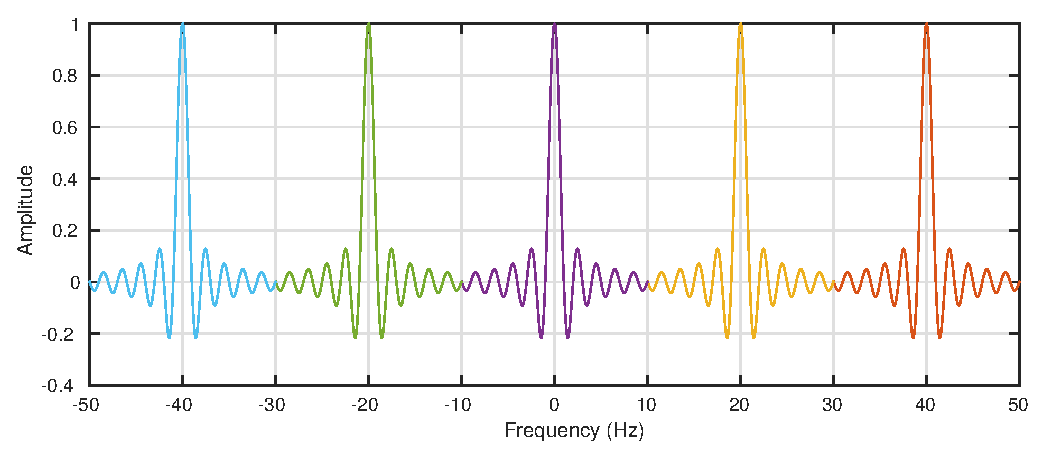
\includegraphics[width=0.9\textwidth]
      {./figures/spectrum_example_fdm}
%     \rule{35em}{0.5pt}
  \caption{Spectrum of a Multicarrier communication scheme}
  \label{fig:multicarrier_fdm_spectrum}
\end{figure}


Another type of multicarrier system that has some advantages over the multicarrier systems shown is called  Orthogonal Frequency Division Multiplexing (\ac{ofdm}). In OFDM, carriers are orthogonal among them, which saves bandwidth since its spectrum overlap.  Figure \ref{fig:multicarrier_ofdm_spectrum} shows the frequency spectrum for an OFDM system with five carriers, it can be seen that the OFDM spectrum uses much less bandwidth when compared with the multicarrier approach shown before. Another advantage of OFDM resides in its implementations. OFDM modems can be realized by means of the Inverse Discrete Fourier Transform \ac{idft} and Discrete Fourier Transforms \ac{dft}, which in turn can be efficiently implemented by the Fast Fourier Transform \ac{fft} making OFDM systems implementation less-complex than that of the multicarrier shown before. Figure \ref{fig:multicarrier_ofdm_diagram} shows the structure of an OFDM modem. Instead of the N filters, decoders and oscillators for every carrier in the parallel communication scheme, only an FFT of N points is used to perform the task. Following, OFDM modulation/demodulation process is described:


\begin{figure}[hbt]
  \centering
    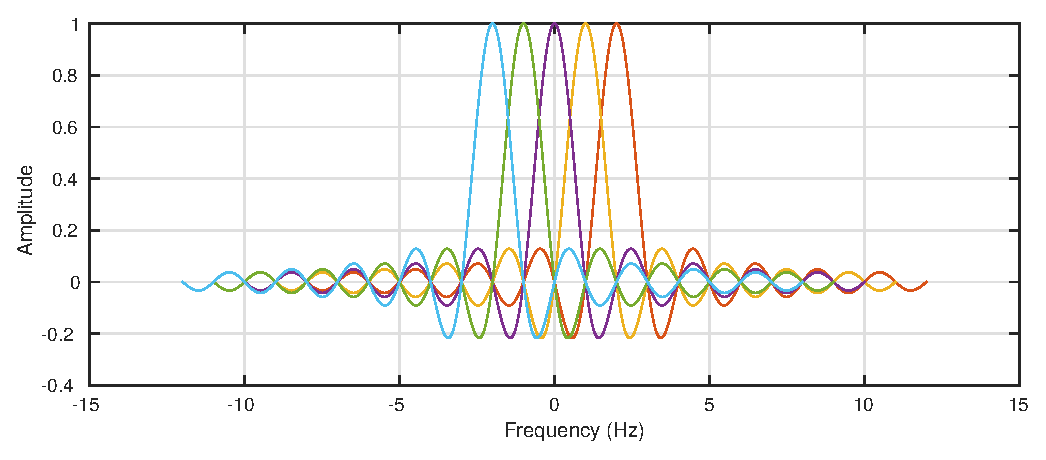
\includegraphics[width=0.9\textwidth]
      {./figures/spectrum_example_ofdm}
%     \rule{35em}{0.5pt}
  \caption{Spectrum of an OFDM communication scheme}
  \label{fig:multicarrier_ofdm_spectrum}
\end{figure}

 
\begin{figure}[hbt]
  \centering
    \includegraphics[width=0.9\textwidth]
      {./figures/multicarrier_diagram_ofdm}
%     \rule{35em}{0.5pt}
  \caption{OFDM basic structure}
  \label{fig:multicarrier_ofdm_diagram}
\end{figure}


 
 
%  The baseband OFDM symbol, in time domain, at the transmitter end, can be expressed as in Eq.\ref{eq:fft_out}, which 
% represents the N-point IFFT of the frequency domain signal, $S_{p}(k)$.
% %%%

% \begin{equation} 
%      x_{p}(n) = \frac{1}{N}\sum\limits_{k=0}^{N-1} S_{p}(k)e^{\frac{j2{\pi}nk}{N}}, \qquad n = 0,1,...,N-1
%     \label{eq:fft_out}
% \end{equation}

%  The transmitted frequency-domain symbol, $S_{p}(k)$, 
% can be recovered by Eq. \ref{eq:fft_out2}, which is the N-point FFT of the transmitted symbol $x_{p}(n)$.
% %%%

% \begin{equation} 
%      S_{p}(k) = \sum\limits_{n=0}^{N-1} x_{p}(n)e^{\frac{-j2{\pi}nk}{N}}, \qquad k = 0,1,...,N-1
%     \label{eq:fft_out2}
% \end{equation}
 
 

%The Orthogonal Frequency Division Multiplexing (OFDM)  technique divides a high data rate stream into several low rate parallel streams, this is achieved by sending every low data rate stream through narrow band flat fading subchannels or subcarriers,  attaining more robustness against ISI since symbol duration is reduced.    


%dividing the frequency selective fading channel into smaller narrow band sub channels, then every low data rate stream is sent in parallel through the subchannels attaining more robustness against Inter symbol Interference (ISI) since symbol duration  %By dividing the available This adds robustness against multi path fading channel, as well as a simpler equalization. 

An OFDM symbol can be described by:


\begin{equation}
S_l(t) = \sum_{k = 0}^{N-1}X_l(k)e^{j2\pi f_kt}, \quad 0 < t < T_s
\label{eq:symbol_ofdm}
\end{equation}

Where, $X_l(k)$ represents the $l_{th}$ OFDM symbol at the $k_{th}$ sub-carrier within an OFDM symbol of duration $T_{s}$ and $\Delta_f$ as the subchannel or subcarrier space for $k = 0, 1, \dotsc, N - 1$. In the OFDM transmission, the information data bits are first mapped into a single carrier symbol, e.g. QAM or QPSK symbols,  and then converted into N parallel streams. This parallel stream of symbols is then carried out by N orthogonal sub-carriers signals whose spectra overlaps in frequency domain achieving high bandwidth efficiency \cite{cho2010mimo}. 

Since it is assumed that the OFDM carriers are orthogonal, two sub-carriers, $\phi_{k}$ and $\phi_{i}$ must met the following condition:

% \begin{align*}
%  \frac{1}{T_s} \int_{0}^{T_s} e^{j2\pi f_kt} e^{-j2\pi f_it} =  \frac{1}{T_s} \int_{0}^{T_s} e^{j2\pi (f_k - f_i)t}   \\
%   =  \frac{1}{T_s} \int_{0}^{T_s} e^{j2\pi (f_k - f_i)t}   \\
%   =  \frac{1}{T_s} \int_{0}^{T_s} e^{j2\pi (f_k - f_i)t}   
% \end{align*}

\begin{align}
  \frac{1}{T_s} \int_{0}^{T_s} \phi_{k}(t) \phi_{i}^{*}(t) dt & = \frac{1}{T_s} \int_{0}^{T_s} e^{j2\pi f_kt} e^{-j2\pi f_it} dt   \nonumber \\   
  & =  \frac{1}{T_s} \int_{0}^{T_s} e^{j2\pi (f_k - f_i)t} dt    \nonumber \\
  & =  \frac{1}{T_s} \int_{0}^{T_s} e^{j2\pi (k-i)\Delta_f}  dt  \nonumber \\
  & =   \delta[k-i].
\label{eq:ortho_signals}
\end{align}

% \begin{eqnarray}
%  \frac{1}{T_s} \int_{0}^{T_s} e^{j2\pi f_kt} e^{-j2\pi f_it} dt =  \frac{1}{T_s} \int_{0}^{T_s} e^{j2\pi (f_k - f_i)t} dt  \\
%   =  \frac{1}{T_s} \int_{0}^{T_s} e^{j2\pi (k-i)\Delta_f}  dt \nonumber \\
%   =   \delta[k-i] \nonumber 
%   \label{ortho_signals}
% \end{eqnarray}


The function $\delta[k-i]$ is defined as:


\begin{equation}
\delta[n] = 
\begin{cases}
1, \quad if \quad n = 0\\
 \\
0, \quad otherwise
\end{cases}
\end{equation}

At the receiver the signal can be recovered using the orthogonality property of equation~\ref{eq:ortho_signals}, as shown in equation~\ref{eq:demod_ofdm}, where $S_r(t)$ is the received signal and $S_l(t)$ the sent signal: 

\begin{align}
S_r(t) & = \frac{1}{T_s} \int_{0}^{k = 0} S_l(t)e^{-j2\pi f_kt} dt \\
 & = \frac{1}{T_s} \int_{0}^{k = 0} \sum_{i = 0}^{N-1}X_le^{j2\pi f_it}e^{-j2\pi f_kt} dt \nonumber \\ 
 & = \sum_{i = 0}^{N-1}X_l\delta[i - k] \nonumber \\ 
 & = X_l . \nonumber \\ 
\label{eq:demod_ofdm}
\end{align}


Sampling the OFDM symbol at intervals of $\frac{T_s}{N}$ yields:


\begin{equation}
S_l(n) = \sum_{k = 0}^{N-1}X_le^{j2\pi f_k n\frac{T_s}{N}  } .
\label{eq:symbol_ofdm_discrete}
\end{equation}

If $f_0 = 0$ then, $f_kT_s = k$ 

\begin{equation}
S_l(n) = \sum_{k = 0}^{N-1}X_le^{j2\pi n\frac{k}{N}  } .
\label{eq:symbol_ofdm_idft}
\end{equation}

Equation \ref{eq:symbol_ofdm_idft} is known as the IDFT of $X_l$. Thus, the OFDM modulation/demodulation can be implemented as a IDFT/DFT pair as shown in figure \ref{fig:multicarrier_ofdm_diagram}. As mentioned before, this simplifies the OFDM transmitter/receiver complexity since no filters or encoders/decoders are used in the modulation/demodulation process. Instead IDFT/DFT are used, which that can be computed efficiently by the FFT algorithm. 

OFDM signals often show bandwidth spillage or leakage, which causes adjacent channel interference (\ac{aci}), since sub-carriers are time limited and no band limited. To avoid \ac{aci}, null carriers are added at the edges of the OFDM symbol. Null carriers at the adjacencies of the OFDM symbol also protect the OFDM signal from leakage from other adjacent systems. In general, another null sub-carrier is the Direct Current (\ac{dc}) sub-carrier, this null sub-carrier corresponds to the zero frequency sub-carrier. If the signal is not modulated, this null subcarrier is added to avoid a DC in the OFDM symbol. This helps in the Digital to Analog and Analog to digital conversion~\cite{nuaymi2007wimax}. Figure \ref{fig:ofdm_symbol_freq} shows an OFDM symbol with 64 sub-carriers in frequency domain, DC, guard band and data carriers are shown in the figure. 

\begin{figure}[hbt]
  \centering
    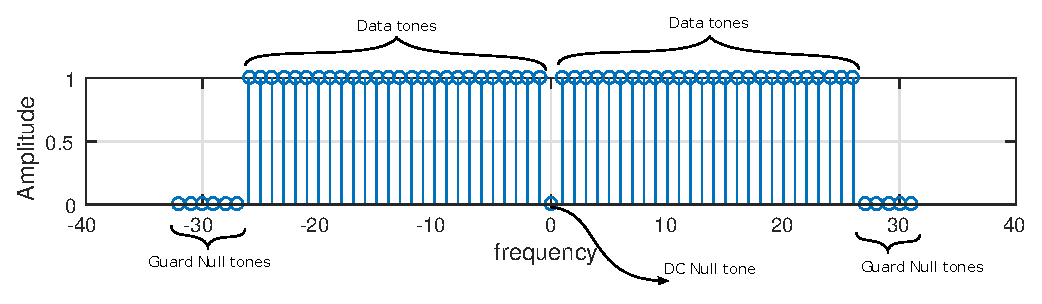
\includegraphics[width=0.9\textwidth]
      {./figures/ofdm_symbol_freq}
%     \rule{35em}{0.5pt}
  \caption{OFDM symbol with 64 sub-carriers in frequency domain}
  \label{fig:ofdm_symbol_freq}
\end{figure}

Another modification that is performed over the OFDM symbol in time domain, is that a copy of the last $G$ samples of the OFDM symbol is prepended to itself, to prevent Inter Symbol Interference (\ac{isi}). The prepended part is known as the Cyclic Prefix (\ac{cp}). ISI is originated by the multi-path fading channel, that causes that a delayed, attenuated and phase shifted copy of the previously sent signal to interfere with the arriving signal. The receiver signal can be modeled by in time domain as:

%and as in equation~\ref{eq:symbol_rx_chnnl_noise} in frequency domain.


%arrives at the receiver, interfering with the arriving signal. 


\begin{eqnarray}
y(n) = {x(n)*h(n)} + z(n) = \sum_{m=0}^{\infty}{x(m)h(n-m)} + z(n).
\label{eq:symbol_ofdm_channel}
\end{eqnarray}

\noindent where, $y(n)$ is the received signal, $x(n)$ the sent signal, and $h(n)$ the impulse response of the multi-path fading channel. The effect of multi-path channel is illustrated in figure~\ref{fig:isi_symbols}. There we see the delayed sent signal overlapping with the current received symbol and interfering with the next symbol at the receiver. The received signal in frequency domain is represented by equation~\ref{eq:symbol_rx_chnnl_noise_freq}.  

\begin{align}
Y(k) & = \sum\limits_{n= 0}^{N-1} [ {x(n)*h(n)} + z(n) ] e^{\frac{-j2{\pi}kn}{N}} \\ 
& = \sum\limits_{n= 0}^{N-1} [ \sum_{m=0}^{N-1}{x(n)h(n-m)} + z(n) ] e^{\frac{-j2{\pi}kn}{N}} \nonumber \\ 
&  = \sum\limits_{m= 0}^{N-1} \sum_{n=0}^{N-1}{x(m)h(n-m)} e^{\frac{-j2{\pi}kn}{N}} + Z(k) \nonumber \\
&  = \sum\limits_{m= 0}^{N-1} x(m) \underbrace{\sum_{n=0}^{N-1}{h(n-m)} e^{\frac{-j2{\pi}kn}{N}}}_{DFT circular shift property} + Z(k) \label{eq:circ_conv_dft_circ_shift} \\
&  = \sum\limits_{m= 0}^{N-1} {x(m)H(k)}e^{\frac{-j2{\pi}km}{N}} + Z(k) \nonumber \\
&  = H(k) \sum\limits_{m= 0}^{N-1} {x(m)}e^{\frac{-j2{\pi}km}{N}} + Z(k) \nonumber \\
&  = X(k)H(k) + Z(k) 
\label{eq:symbol_rx_chnnl_noise_freq}
\end{align}


According to equation~\ref{eq:symbol_rx_chnnl_noise_freq}, the channel compensation can be accomplished by simply dividing the received symbol in frequency domain by the channel response, i.e. $X(k) = Y(k)/H(k)$, which represents a one tap equalizer. Also $Y(k)=X(k)H(k)$ is true only when $ y(n) = x(n) \circledast y(n)$, where $\circledast$ denotes circular convolution. This makes possible to apply the DFT circular shift property in equation~\ref{eq:circ_conv_dft_circ_shift}, the circular convolution holds true only when the CP is prepended to the OFDM symbol \cite{cho2010mimo}.

%According to equation~\ref{eq:symbol_rx_chnnl_noise_freq} result, the channel compensation can be accomplished by simply dividing the received symbol in frequency domain by the channel response, that is $X(k) = Y(k)/H(k)$, which represents a one tap equalizer. Also $Y(k)=X(k)H(k)$ is true only when $ y(n) = x(n) \circledast y(n)$, where $\circledast$ denotes circular convolution (Convolution theorem), this makes possible to apply the DFT circular shift property in equation~\ref{eq:circ_conv_dft_circ_shift}, this relationship holds true only when the CP is prepended to the OFDM symbol \cite{cho2010mimo}.


\begin{figure}[hbt]
  \centering
    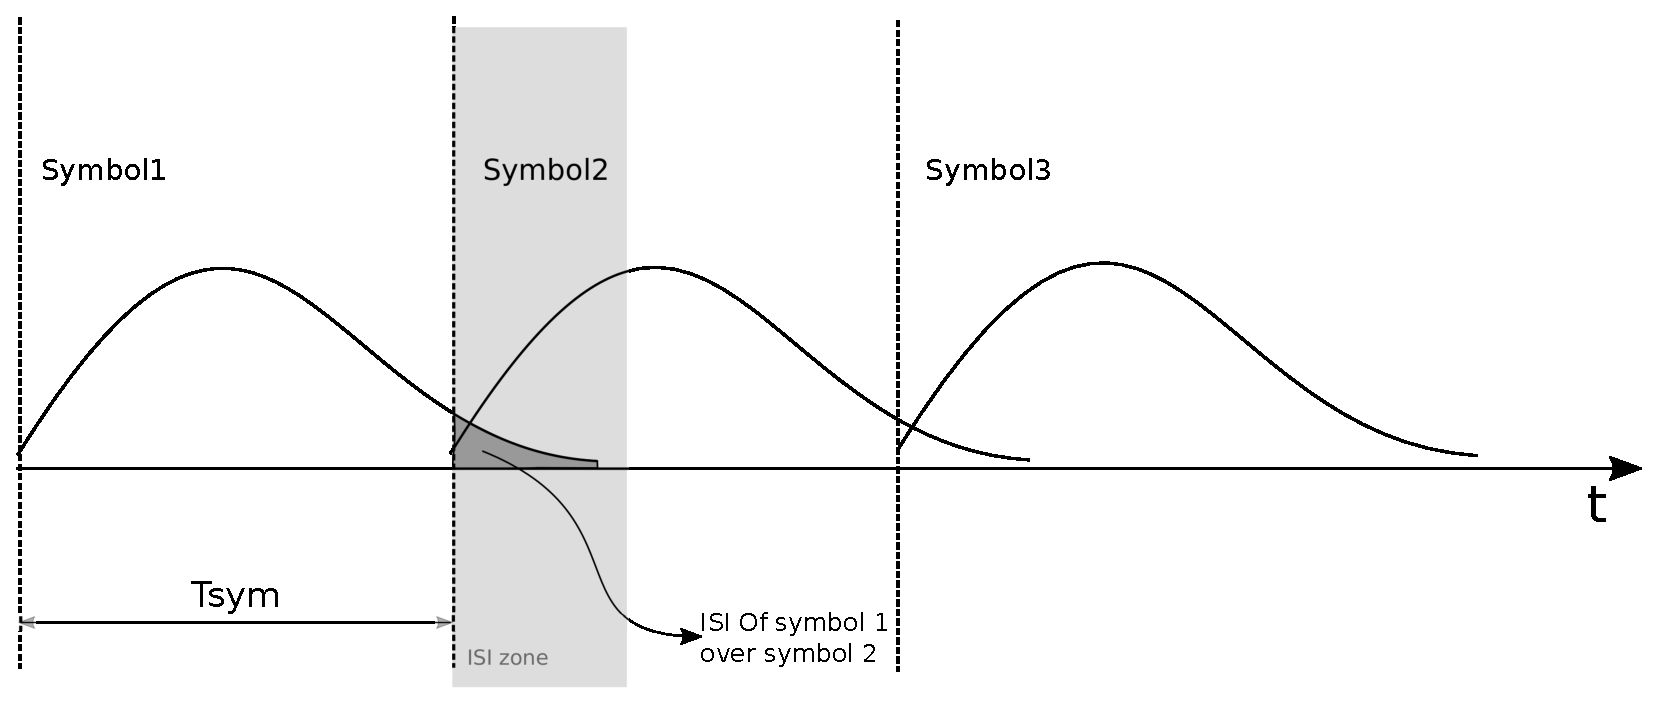
\includegraphics[width=0.8\textwidth]
      {./figures/isi_fig}
%     \rule{35em}{0.5pt}
  \caption{ISI effect over adjacent symbols}
  \label{fig:isi_symbols}
\end{figure}

 The CP appended to the beginning of the OFDM symbol in time domain safeguards the OFDM symbol from being affected by the multi-path fading channel effect over the previous transmitted symbol, as long as the channel delay is shortest than that of the duration of the CP. Figure \ref{fig:isi_symbols_cp} illustrates the effect of ISI over the OFDM symbol when the CP is added. 

\begin{figure}[hbt]
  \centering
    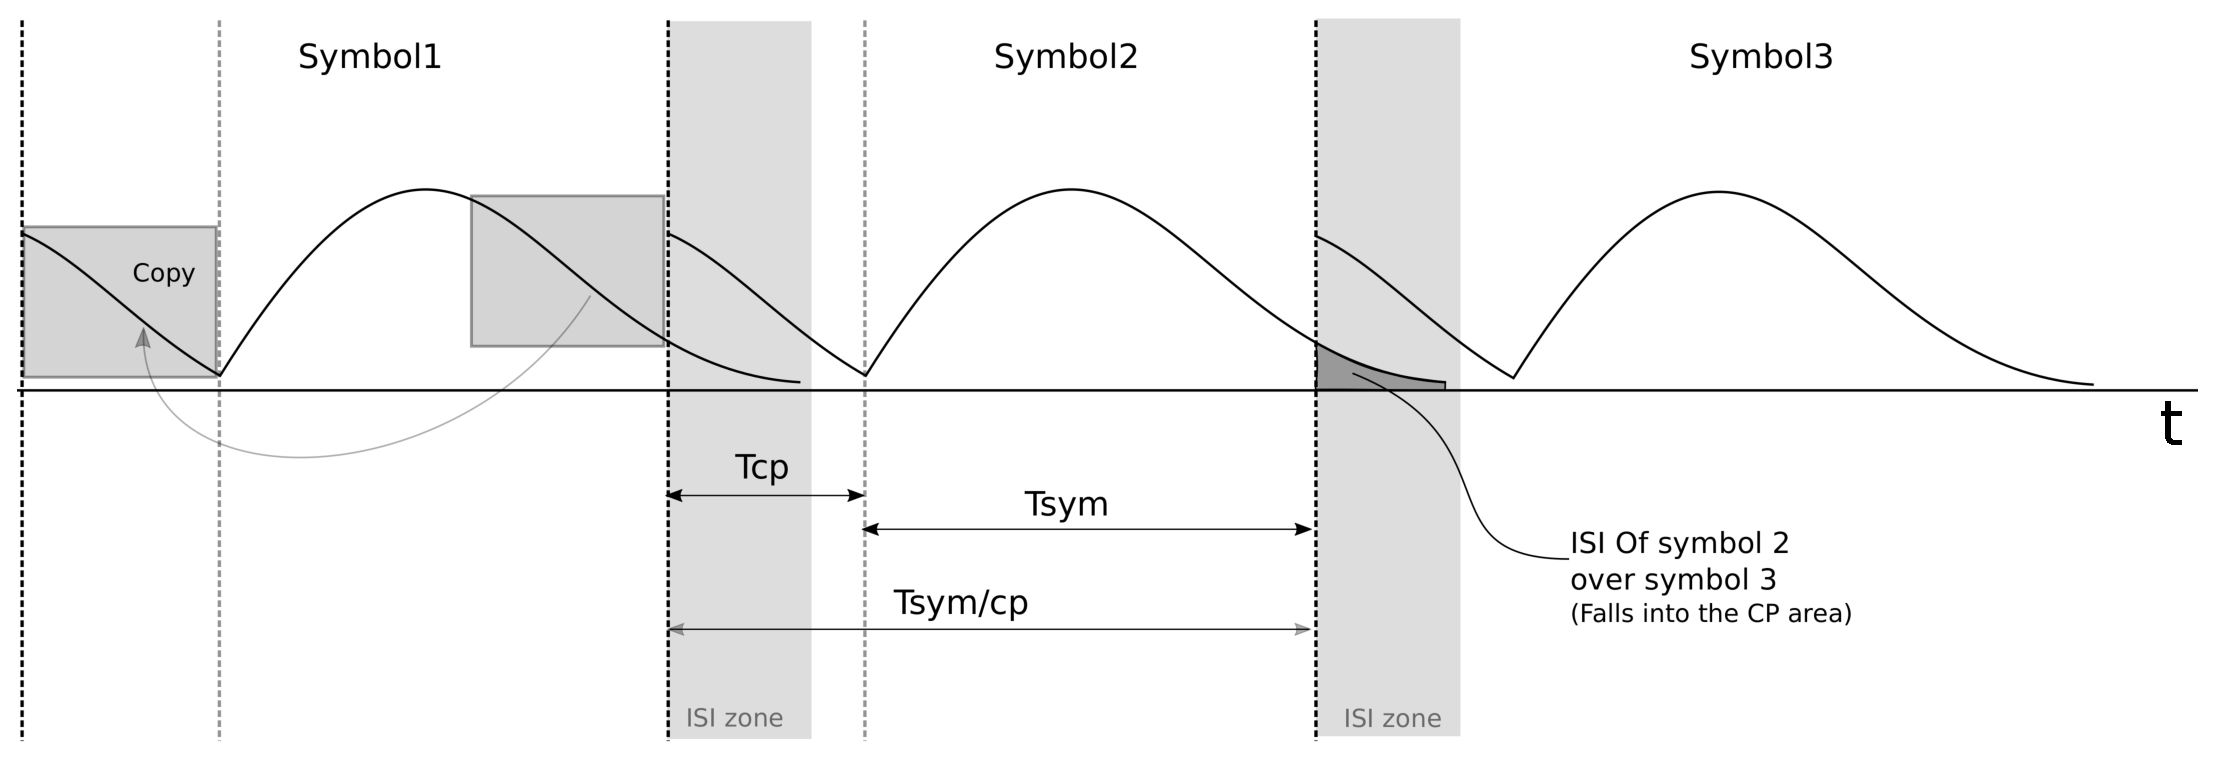
\includegraphics[width=0.9\textwidth]
      {./figures/isi_cp_2}
%     \rule{35em}{0.5pt}
  \caption{ISI effect over adjacent symbols with CP}
  \label{fig:isi_symbols_cp}
\end{figure}


\subsection{Synchronizations Errors in OFDM}

Although OFDM is widely used due to its robustness against frequency-selective fading channel as well as the reduced complexity single-tap equalizer per subcarrier \cite{chiueh2012baseband} it has large Peak to Average Ratio (PAPR)~\cite{prasad2004ofdm} and is very sensitive to the receiver synchronization errors~\cite{ber_cfo_ofdm}, such as Symbol Time Offset (\ac{sto}), i.e. finding the start of the OFDM symbol unknown at the receiver, and Carrier Frequency Offset (CFO) caused mainly by the frequency mismatch between local oscillators at the receiver and transmitter. Synchronization errors as STO and ICFO can cause Inter Symbol Interference (ISI) and Inter Carrier Interference (ICI) that hinders the proper recovery of the OFDM symbols and degrades system performance. Thus, the receiver must estimate and compensate those errors in order to properly recover the symbols. Following, the effects of those errors over the OFDM symbols are analyzed. 


\subsubsection{Carrier Frequency Offset}
\label{sec:icfo}

 
 The tolerance of local and remote oscillators causes a difference between the transmitter and receiver carrier frequency. This difference in frequencies, known as carrier frequency offset (\ac{cfo}), has some detrimental effect on sub-carriers,  hindering the symbols recovery. It can be divided into two parts regarding the sub-carrier space, a fractional frequency offset, which is a fraction of the sub-carrier spacing, and an Integer Carrier Frequency Offset (ICFO) which occurs in multiples of the sub-carriers distance.   
    
  The fractional part causes Inter Carrier Interference (\ac{ici}) due to lost of orthogonality between sub-carriers. It is typically corrected in two steps, first a coarse estimation/correction is performed followed by a fine frequency estimation/correction. On the other hand, the integer part causes a circular shift of the sub-carrier indexes in the frequency domain. It is usually estimated in frequency domain and its correction can be performed either in time or frequency domain. 

Assuming perfect symbol synchronization, i.e. zero Symbol Time Offset (the frame start is perfectly located), and without considering the impairments introduced by the channel, the transmitted symbol is frequency domain is described by equation \ref{eq:symbol_freq}, while received symbol in time domain can be described by Eq.~\ref{eq:ifft_cfo}. 
%, it is given by the IFFT of the \emph{p-th} symbol in frequency domain shifted by $\beta$.  

\begin{equation} 
     X_{p}(k) = \sum\limits_{n=0}^{N-1} x_{p}(n)e^{\frac{-j2{\pi}kn}{N}}, \qquad k = 0,1,...,N-1
    \label{eq:symbol_freq}
\end{equation}



\begin{equation} 
     y_{p}(n) = \frac{1}{N}\sum\limits_{k=0}^{N-1} X_{p}(k+\beta)e^{\frac{j2{\pi}kn}{N}}, \qquad n = 0,1,...,N-1
    \label{eq:ifft_cfo}
\end{equation}


\noindent where $\beta = \epsilon + k_{o}$ is the frequency offset, divided in $\epsilon$, the fractional frequency offset and $k_{o}$ the integer frequency offset. $X_p(k)$ the transmitted symbol in frequency domain with $k$ sub-carriers, $x_p(n)$ in time domain and $y_p(n)$ the received signal in time domain. Assuming a fractional frequency offset of zero ($\beta = k_{o}$), the term $X_{p}(k+\beta)$ can be written as in eq.~\ref{eq:ifft_symbol_shifted}

\begin{equation} 
X_{p}(k+\beta) = \sum\limits_{b=0}^{N-1} x_{p}(b)e^{\frac{-j2{\pi}(k+\beta)b}{N}}, \qquad k+\beta = 0,1,...,N-1 .
    \label{eq:ifft_symbol_shifted}
\end{equation}

% \begin{equation} 
%      r_{k} = e^{\frac{j2{\pi}n(k_{o}+\epsilon)}{N}}\sum\limits_{m=0}^{q} x_{k}h_{m} + n_{k}, 
%     \label{eq:symb_rx}
% \end{equation}
So, Eq.~\ref{eq:ifft_cfo} can be written as: %Eq.~\ref{eq:ifft_cfo_symbol_shifted}

\begin{equation} 
     y_{p}(n) = \frac{1}{N}\sum\limits_{k=0}^{N-1} \Big\{ \sum\limits_{b=0}^{N-1} x_{p}(b)e^{\frac{-j2{\pi}(k+\beta)b}{N}} \Big\} e^{\frac{j2{\pi}kn}{N}}, \qquad n = 0,1,...,N-1.
    \label{eq:ifft_cfo_symbol_shifted}
\end{equation}

\begin{equation} 
     y_{p}(n) = \frac{1}{N}\sum\limits_{b=0}^{N-1}x_{p}(b)e^{\frac{-j2{\pi}\beta b}{N}} \sum\limits_{k=0}^{N-1} e^{\frac{j2{\pi}k(n-b)}{N}} , \qquad n = 0,1,...,N-1.
    \label{eq:ifft_cfo_symbol_shifted_2sum}
\end{equation}


%%%%%%%%%%%%OJO LEER Y REDACTAR DE NUEVO%%%%%%%%%%%%%%%%%%%%%%%%%%%%%%%%%%%%%%%%%%%%%%

%If the index $b = n$ then, the variable $b$ in the first summation becomes a constant, and the complex variable exponent in the second summation becomes zero, given N as the summation result. The $p^{th}$ symbol in time domain can be expresed as eq.~\ref{}

%%%%%%%%%%%%%%%%%%%%%%%%%%%%%%%%%%%%%%%%%%%%%%%%%%%%%%%%%%%%%%%%%%%%%%%%%%%%%%%%%%%%%%%

If the index $b = n$, then the $p_{th}$ symbol in time domain can be expressed as eq.~\ref{eq:ifft_cfo_symbol_shifted_time}

\begin{equation} 
     y_{p}(n) = x_{p}(n)e^{\frac{-j2{\pi}\beta n}{N}}, \qquad n = 0,1,...,N-1.
    \label{eq:ifft_cfo_symbol_shifted_time}
\end{equation}

% %where, $n_{k}$ is the noise sample, $h$ is the channel impulse response, $\epsilon$ is a
% normalized fractional carrier frequency offset and $k_{o}$ is the normalized ICFO, which is the impairment to be 
% tackled by the algorithm that will be presented in section~\ref{sec:fft_cfo_architecture}. The presence of ICFO causes an incorrect tone numbering at the FFT output,

From eq.~\ref{eq:ifft_cfo_symbol_shifted_time} can be concluded that, the received symbol has the same value than that of the transmitted symbol with its phase rotated by $-j 2 \pi  \beta n/N$. As the fractional part is equal to zero, the integer frequency offset effect over the sub-carriers in frequency domain is a shift, as shown in the illustrative example of figure \ref{fig:icfo_example}.  
 
 \begin{figure}[hbt]
  \centering
    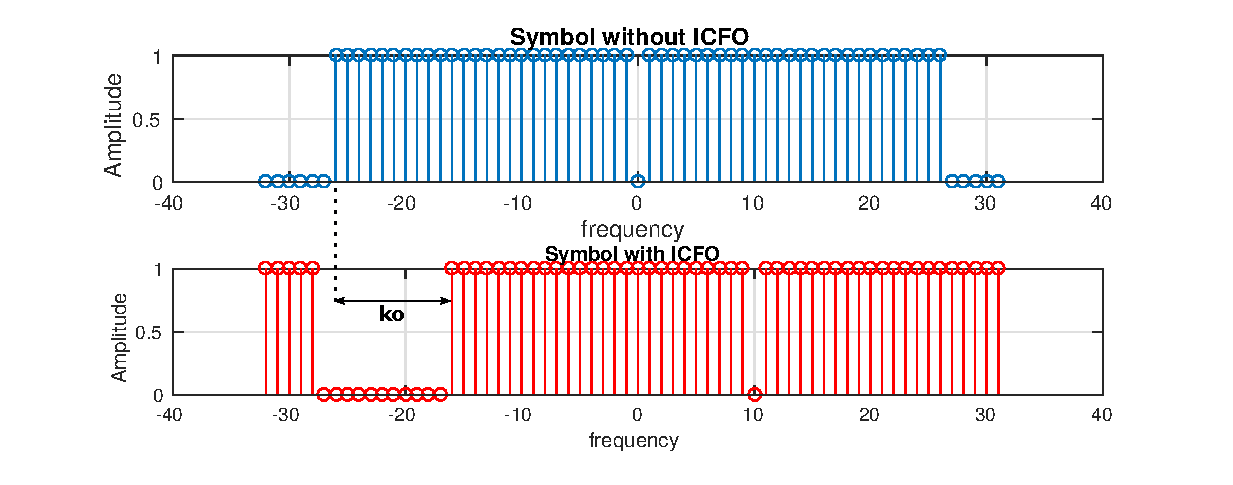
\includegraphics[width=1\textwidth]
      {./figures/icfo_shift}
%     \rule{35em}{0.5pt}
  \caption{Integer Carrier Frequency Offset of $k_{o}$ subcarriers - without error(top), with error (bottom)}
  \label{fig:icfo_example}
\end{figure}

 \subsubsection{Symbol Time Offset}
\label{sec:symbol_time_offset}

  Another impairment regarding synchronization is the symbol time synchronization error. Timing synchronization algorithms attempt to find the start of the OFDM symbol and correct what is called the STO, defined as the difference between the exact symbol start and the estimated one. The STO must be zero, so that the result of the FFT computation matches that of the transmitted symbol in frequency domain. 
  
  
  \begin{figure}[!hbt]
  \centering
    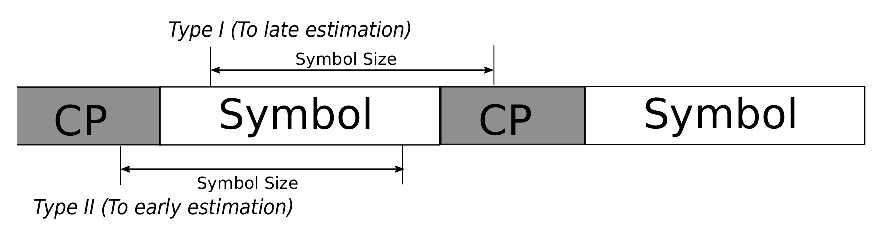
\includegraphics[width=0.8\textwidth]
      {./figures/STO_symbol}
%     \rule{35em}{0.5pt}
  \caption{STO early and late estimation}
  \label{fig:sto_estimation}
\end{figure}


 A deviation from the ideal STO can be found after the estimation process as shown in figure~\ref{fig:sto_estimation}. STO can be estimated to early or to late, regarding the ideal case in which the exact point is expected to be. A late estimation (type I, as shown in figure \ref{fig:sto_estimation}), which takes the starting point after the ideal case, generates a time windows that is shifted onto the next symbol, that is, samples from the current symbol are lost and samples from the next symbol are taken. In this case ICI is found and the orthogonality between sub-carriers is lost~\cite{cho2010mimo}. 


  The second type of offset found is the one in which the starting point is estimated to early (type II, in figure~\ref{fig:sto_estimation}), that is before the ideal starting point. In this case the first sample of the symbol falls inside the symbol CP and the last samples are lost, no samples from the next symbols are taken. In this case, the orthogonality between sub-carriers is preserved and only a phase offset proportional to the STO and the carrier index is shown in the post-FFT signal~\cite{cho2010mimo}.
  
If the STO falls inside the CP of the current symbol, and without considering the impairments introduced by the channel, the received signal can be expressed as:

\begin{equation} 
     S_{p}(k) = \sum\limits_{n=0}^{N-1} x_{p}(n+\alpha)e^{\frac{-j2{\pi}nk}{N}}, \qquad k = 0,1,...,N-1
    \label{eq:symbol_rx_sto}
\end{equation}

\noindent where the shifted symbol then can be rewritten  as:

\begin{equation} 
x_{p}(n+\alpha) = \sum\limits_{b=0}^{N-1} X_{p}(b)e^{\frac{j2{\pi}(n+\alpha)b}{N}}, \qquad b = 0,1,...,N-1
    \label{eq:fft_symbol_shifted_time}
\end{equation}

Substituting equation~\ref{eq:fft_symbol_shifted_time} in equation~\ref{eq:symbol_rx_sto} we obtain:


\begin{equation}
     S_{p}(k) = \sum\limits_{n=0}^{N-1} \Big\{ \sum\limits_{b=0}^{N-1} X_{p}(b)e^{\frac{j2{\pi}(n+\alpha)b}{N}}  \Big\} e^{\frac{-j2{\pi}nk}{N}}
    \label{eq:symbol_rx_sto_2}
\end{equation}

Rearranging equation~\ref{eq:symbol_rx_sto_2},  

\begin{equation}
  S_{p}(k) = \sum\limits_{b=0}^{N-1} X_{p}(b)e^{\frac{j2{\pi}\alpha b}{N}} \sum\limits_{n=0}^{N-1} e^{\frac{j2{\pi}n(b-k)}{N}}
    \label{eq:symbol_rx_sto_3}
\end{equation}

If $b = k$ then, equation~\ref{eq:symbol_rx_sto_3} becomes

\begin{equation}
  S_{p}(k) = X_{p}(b)e^{\frac{j2{\pi}\alpha b}{N}}
    \label{eq:symbol_rx_sto_4}
\end{equation}


That is, at the receiver, the same carrier in frequency domain of the transmitter is modified in phase by a factor equal to $\frac{j2{\pi}\alpha b}{N}$, i.e. ,STO only introduces a phase shift in frequency domain if the STO is smaller than the CP size and of type II. 


 STO of type I cannot be reversed because the start frame decision is already made and samples before the symbol start are discarded, on the contrary, type II STO errors can be reversed as this kind of error only shows changes in signal phase, however time offset grater than certain values degrade significantly the signal if samples of the cyclic prefix are affected by previous symbols due to the multipath fading channel~\cite{canet2007time}, even if it falls inside the CP.

There exist several methods estimate and correct timing errors and frequency errors based on repetitive structures inherent in the OFDM symbol (as the CP case). Known as Non-Data-Aided methods or blind methods, these algorithms save bandwidth, since no structure must be sent to estimate the errors. Frame oriented systems benefit from this type of algorithms, since the estimation is performed continuously. A second kind of estimation based on a known sequence sent in the PPDU can be employed. This kind of algorithms, known as data-aided, consumes more bandwidth but prove to be more robust than the non-data aided methods. Packet based system benefit from this kind of estimation. Those algorithm will be reviewed in future chapters. 






%OFDM is widely used due to its robustness against frequency-selective fading channel as well as the reduced complexity single-tap equalizer per subcarrier. However, it has large Peak to Average Ratio (PAPR)~\cite{prasad2004ofdm} and is very sensitive to the receiver synchronization errors~\cite{ber_cfo_ofdm}, such as Symbol Time Offset (\ac{sto}) i.e. finding the start of the OFDM symbol, unknown at the receiver and Carrier Frequency Offset (CFO) caused mainly by the frequency mismatch between local oscillators at the receiver and transmitter.



%%%


  \chapter{IEEE802.15.4g standard }

IoT is a new paradigm in which everyday objects are connected to the Internet. In this evolution of the Internet, conventional objects are granted smart capabilities, allowing them to sense environmental changes, send and receive data and perform tasks. This new network of smart objects opens up a myriad of applications: smart cities, that employ adaptive lighting to optimize energy consumption; smart parking that notifies of available parking spaces; warnings of climate changes; also in healthcare, for remote monitoring of patients and monitor and tracking of vital signs; smart utility networks and smart metering for monitoring of water, oil and gas levels in storage tanks; smart grid for monitoring and management of the electrical system. 

Since the range of applications is very wide, and smart devices are composed of several complex components, major vendors of specific areas are developing their own solutions isolated. Thus, the success of this new technology relies to a large extent on standardization, that will guarantee interoperability, portability, and manageability between devices from different vendors. 

An important feature of the IoT device is its ability to communicate with others devices. The data exchange allows to make decision-based on status, environmental changes etc. Several communications protocols are being used for the IoT, its main features are low-data rates with low power and implementation costs. The following are some of the communications protocols being used in IoT devices:


\begin{itemize}
\item \emph{ZigBee} It is based on the IEEE802.15.4 standard, a standard that defines the operation of LR-WPANs. It specifies the requirements for a low-cost low-power mesh network, it is designed to carry small amounts of data over a short distance while consuming very little power. ZigBee  operates  on the 2.4 Ghz frequency band as well as in the 800-900 sub-GHz bands. 

\item \emph{LoRaWan (Long Range Wide Area Network)}  Developed for long distance networks for national, regional or global areas. Composed mainly of wireless devices powered by batteries. It features bidirectional communications as well as low power consumption, some of the IoT requirements.  

\item \emph{Sigfox}. The basic idea of this technology is to have base stations distributed across some small area and simple devices that can exchange messages with them. A Sigfox message has up to 12-bytes payload and its frame will use 26 bytes in total. It relies on The Ultra Narrow Band modulation technology to exchange messages over the air. Devices requirements are low-power and low-cost. 

\item \emph{WI-SUN}, backed by the Wi-SUN alliance, this technology features low data rates, low power, short-range communication with very low implementation complexity. The Wi-SUN alliance defines the Wireless Smart Ubiquitous Network (Wi-SUN) as a technology
based on the IEEE 802.15.4g standard, an amendment of the IEEE802.15.4 standard. Two profiles are defined by the Wi-SUN Alliance, FAN and HAN networks that support both star and mesh topologies. The communication range is usually from 10 to 75m with low data rate of tens of kbps up to 250 kbps~\cite{sato2015smart}. 

\end{itemize}

%To be able to perform the required tasks, smart objects must be equipped with 
% The Internet of Things is basically a network of interconnected smart objects. In this new kind of network everyday objects will be granted computational and communication capabilities, smart objects will be an integration of several technologies. Thus, expanding its range of application. Based on this concept a myriad of applications appear, smart cities, healthcare, smart homes. The success of this new technology relies on standardization ( Cisco and Forber predicting that the IoT could grow between 50 and 40 billion objects connected by 2020 \cite{forbes}, \cite{cisco}) since it is a growing filed the numbers of solution is rapidly increasing. Standardization will guarantee levels of interoperability, portability and manageability between devices from different vendors. 

%An IoT smart device must be equipped with a processing unit, that process data, sensors and actuators that gathers environmental data and performs specific task. A communication unit that send and receive information from others or to others smart devices. 

%Low power consumption is a must in this smart devices, since they run on batteries most of the time. Thus, hardware and software should be designed to extend battery life to its maximum. 


%SMART GRID     %SMART UTILITY NETWORK = SMART METERING UTILITY NETWORK
%(ELECTRICIDAD) % (SE REFIERE A MEDICION Y COMUNICACION)
%A example of an application for IoT is the Smart Grid. The electrical grid is provided with smart capabilities allowing a two way communication between the customer and the provider. In smart grids smart devices will sense the status of the electrical network, sent data to operation centers and perform managements based on gathered data. Smart metering utility networks (SUNs) enable system control and information transfer in smart grid.  

%Formerly devoted to Smart Metering Utility Network applications and now employed in Smart Ubiquitous Networks (\ac{sunnet}), 

The IEEE 802.15 Working Group for Wireless Specialty Networks developed the 15.4g standard, featuring low-rate wireless connectivity with low power consumption and short-range communication. The IEEE 802.15.4g standard defines Physical (\ac{phy}) and Media Access Control (\ac{mac}) layers requirements for Low-Rate Wireless Personal Area Networks (\ac{LoWPANs}). The next section describes the IEEE802.15.4g standard and some of its features.
%\section{IOT needs standards to be able to live within all the industries that are developing IOT smart devices}

%\subsection{An IOT device has a communication element}

%\subsection{Example of applications Smart Grid}

\section{IEEE802.15.4g Standard}


The IEEE802.15.4g standard is an amendment to the
IEEE802.15.4. It defines alternate PHYs in addition to those in the IEEE802.15.4 as well as modulations,
 data rates, frequency bands and other technical properties. %It enables communication between smart meters and smart grid devices as well as smart home appliances~\cite{anton2014machine}. 

Three PHYs are defined in the IEEE802.15.4g standard:
1) the Multi-rate and 
Multi-Regional Frequency Shift Keying (\ac{fsk}) PHY, with data rates ranging from 50 Kbps to 400 kpbs provides good transmit power efficiency due to the constant envelope of the transmit signal ~\cite{sun_std_2012}, shows low implementation complexity and supports various frequency bands including Europe, Canada, U.S, Korea and Worldwide; 2) The Multi Rate and Multi-Regional Offset Quadrature Phase-Shift Keying  (\ac{qpsk})
PHY shows similar features to those of the IEEE 802.15.4-2011 \ac{qpsk} PHY, thus,  it guarantees interoperability between previously developed devices, it supports Direct Sequence Spread Spectrum (\ac{dsss}) and Multiplexed Direct Sequence Spread Spectrum (\ac{mdsss}). The Multi-Rate and Multi-Regional Orthogonal Frequency Division Multiplexing (\ac{ofdm}) PHY, which provides
 the highest data rates of the three PHYs at the cost of a more complex structure and implementation, it supports data rates ranging from 50 Kpbs to 800 Kbps~\cite{sun_std_2012}. Since the current focus of this work is the development of block concerning the MR-OFDM PHY a more detailed description will be presented in the next section. 
 
\subsection{IEEE802.15.4g MR-OFDM}
\label{sec:mr_ofdm}
%Since the focus of this work is the implementation of blocks concerning the 
%.\ac{ofdm} mode it will be described in detail in this section.



An OFDM modulator can be implemented as an N-point IDFT (see Fig.~\ref{fig:ofdm_tx}), which converts data sequences from frequency domain to time domain, while the demodulator
can be performed by a DFT (see Fig.~\ref{fig:ofdm_rx}) , where each block of N 
received samples is converted back to the frequency domain.
It is well known that the implementation of IDFT/DFT consumes a lot of resources, making mandatory 
the use of the Fast Fourier Transform (\ac{fft}) algorithms, which is one of the addressed topics in this work. 


The MR-OFDM mode as specified in~\cite{sun_std_2012} supports \ac{bpsk}, \ac{qpsk2} and 16-\ac{qam} modulations, depending on the Modulation and Coding Scheme (\ac{mcs}) chosen. Channel encoding is mandatory with a convolutional encoder of coding rate $R =1/2$, it can be punctured to achieve $R = 3/4$. With  \ac{dft} sizes of 128, 64, 32 and 16, the data rates for MR-OFDM ranges from 50 kbps to 800 kbps. Table~\ref{table_mrofdm} shows a summary of the main parameters for the OFDM mode. 

%\begin{table}[htb!]\tiny
\begin{table}[htb!]\footnotesize
\caption{Main Parameters of the MR-OFDM Mode}
\label{table_mrofdm}
\centering
\begin{tabular}{@{}c c c c c c}
\hline
\textbf{PARAMETER}	&\textbf{OPTION 1}	&\textbf{OPTION 2}	&\textbf{OPTION 3}	&\textbf{OPTION 4}	&\textbf{UNIT}\\
\hline\\
SAMPLING RATE		&$1.333\overline{3}$	&$0.666\overline{6}$	&$0.333\overline{3}$ 	&$0.166\overline{6}$	&MSamples/sec\\
FFT SIZE		&$128$			&$64$			&$32$			&$16$			&$\textendash$\\
TONE SPACING		&$10.416\overline{6}$	&$10.416\overline{6}$	&$10.416\overline{6}$	&$10.416\overline{6}$	&KHz\\
FFT DURATION		&$96$			&$96$			&$96$			&$96$			&$\mu s$\\
GI  LENGTH		&$24$			&$24$			&$24$			&$24$			&$\mu s$\\
SYMBOL DURATION		&$120$			&$120$			&$120$			&$120$			&$\mu s$\\
SYMBOL RATE		&$8.333$		&$8.333$		&$8.333$		&$8.333$		&KSymbols/sec\\
ACTIVE TONES		&$104$			&$52$			&$26$			&$14$			&$\textendash$\\
PILOT/DATA/DC TONES	&$8/96/1$		&$4/48/1$		&$2/24/1$		&$2/12/1$		&$\textendash$\\
BANDWIDTH 		&$1094$ 		&$552$			&$281$			&$156$			&KHz\\
%One & Two\\
%\hline
%Three & Four\\
\hline
\end{tabular}
\end{table}

% The MR-OFDM transceiver  contains the 
% transmitter and receiver blocks presented in Fig.~\ref{fig:ofdm_tx} and 
% Fig.~\ref{fig:ofdm_rx}. The main objective of the transmitter is to encode
% the data that will be transmitted and build the PPDU according to the reference
% modulator given by~\cite{sun_std_2012}. Fig.~\ref{fig:ofdm_ppdu_ltf}
% shows the complete \ac{ppdu} structure, which contains: Synchronization Header (\ac{shr}), composed by
% Short Training Field (\ac{stf}) and Long Training Field (\ac{ltf}); PHY Header (\ac{phr}), 
% which carries frame length, scrambling seed, modulation and coding
% scheme (\ac{mcs}); Packet Service Data Unit (\ac{psdu}), which is the PHY payload; PPDU Tail Bits field (TAIL) and Pad Bits (PAD) field.


The \ac{mrofdm} modulator has to encode the data and build the PPDU 
according to the structure defined in~\cite{sun_std_2012}. The PPDU is 
shown in figure~\ref{fig:ofdm_ppdu_ltf}, it contains: Synchronization 
Header (\ac{shr}) used to estimate channel behavior and correct frequency and timing errors. The \ac{shr} is composed by the Short Training Field (\ac{stf}) and Long
Training Field (\ac{ltf}); PHY Header (\ac{phr}), which carries frame 
length, scrambling seed, modulation and coding scheme (\ac{mcs}); Packet
Service Data Unit (\ac{psdu}), the actual payload; PPDU Tail Bits 
field (TAIL) and Pad Bits (PAD) field used to reset and fill buffers. 

\begin{figure}[hbt]
  \centering
    \includegraphics[width=0.6\textwidth]
     {./figuras/ofdm_ppdu_ltf}
%     \rule{35em}{0.5pt}
  \caption{Format of the MR-OFDM PPDU and LTF}
  \label{fig:ofdm_ppdu_ltf}
\end{figure}


The modulator structure is depicted in figure~\ref{fig:ofdm_tx}. This MR-OFDM PHY was designed at Eldorado Research Institute for the ASIC implementation of the IEEE802.15.4g standard, from the reference structure and specification found in \cite{sun_std_2012}. The figure shows the 
modulator divided in data and signal processing. Within the data processing part, conditioning of data bits is performed, it allows error correction and protect the data from channel impairments. From the 
Mapper (point 9 in figure~\ref{fig:ofdm_tx}) onward, digital signal processing is applied, here
signal conditioning is applied to complex decimal data. Referencing figure \ref{fig:ofdm_tx} every numbered point represents  a conditioning or modification of the data, the complete data processing and signal processing is as follows:

\begin{figure}[hbt]
  \centering
    \includegraphics[width=0.9\textwidth]
      {./figures/OFDM_TX_V4_2}
      %{./figures/OFDM_tx_v1}
%     \rule{35em}{0.5pt}
  \caption{MR-OFDM Modulator according to the IEEE802.15.4g Standard}
  \label{fig:ofdm_tx}
\end{figure}


\begin{itemize}
\item \emph{Modulator Data Processing}

\begin{description}
\item [1. ] \emph{PSDU Data}: The payload is received from the upper MAC layer, that is the information that is going to be modulated, i.e. a string of bits that represent some message.
\item [$\boldsymbol{1^{'}}$.] \emph{Configuration}: Generation of Frame length, MCS Level, Data rate, scrambler seed are configurations that come from the MAC layer.  
\item [2. ] \emph{Padder}: PAD bits and TAILS bits are added through the padder block to the PSDU. 
\item [3. ] \emph{Scrambler}: It randomizes the data bits, avoiding long sequences of zeros or ones.
\item [4. ] \emph{PHR Generator}: It generates the PHR according to the configuration chosen in the MAC layer. 
\item [5. ] \emph{Encoder Handler}: Since not all the data is encoded in the same way, this block exchanges between scrambled data and PHR data, in other words, it controls which data to be encoded.  
\item [6. ] \emph{Encoder}: It adds redundancy to the incoming data to add error correction capabilities to the system. 
\item [7 .] \emph{Puncturer}: It changes the data rate according to the MCS. 
\item [8 .] \emph{Interleaver}: Changes the bits order in the data stream. It avoids burst errors.
\item [9 .] \emph{Mapper}: Converts bits to symbols, it maps data bits to a BPSK, QPSK or 16 QAM symbol according to the MCS adopted. 
\end{description}

\item \emph{Modulator Signal Processing}

\begin{description}
\item [10 .] \emph{Frequency Spreader}: Spread the signal in a frequency band greater than the original signal, replicas of the signal are combined to obtain a single symbol.

\item [$\boldsymbol{10'}$ .] \emph{STF}: Short training field, it adds a known sequence to the beginning of the frame, information that is used at the receiver to estimate and correct timing and frequency errors. 

\item [$\boldsymbol{10'}$ .] \emph{LTF}: Long training field. known sequence different from the STF. Although with the same function, used for syncrhonization, frequency error correction and channel equalization at the receiver.

\item [$\boldsymbol{10'}$ .] \emph{Pilot, DC and Guard}: Pilots tones for channel detection and channel gain estimation, DC tone and guard interval to avoid channel interference.  

\item [11 .] \emph{Framer}: The framer rearranges the complex symbols and prepares the OFDM symbol. 

\item [12 .] \emph{Inverse Fourier Transform}: It converts the symbol from frequency domain  to time domain. 

\item [13 .] \emph{CP Insertion}: Adds a Cyclic Prefix, to eliminate inter symbol interference (ISI).

\end{description}

\end{itemize}



% \begin{figure}[hbt]
%   \centering
%     \includegraphics[width=0.9\textwidth]
%       {./figuras/OFDM_DEMO_V_TX_V3}
%       %{./figures/OFDM_tx_v1}
% %     \rule{35em}{0.5pt}
%   \caption{MR-OFDM transmitter according to the IEEE802.15.4g}
%   \label{fig:ofdm_tx}
% \end{figure}

Fig. ~\ref{fig:ofdm_rx} depicts the demodulator structure, its main goal is to   
recover the transmitted data. Basically the receiver undo the process done by the transmitter, however, before this can be accomplished, it has to deal with synchronization issues. Timing synchronization must be attain as well as frequency errors corrected to revert the process done in the transmitter. This is why almost all the signal processing part of the receiver is dedicated to synchronization and frequency error correction. Frequency synchronization and its implementation is one of the topics of this work, specific on the Integer Carrier Frequency Offset (\ac{icfo}) which is estimated and corrected by the block highlighted in Fig.~\ref{fig:ofdm_rx}. A detailed description of the ICFO is found in section~\ref{sec:icfo}. The processing involved at the demodulator is as follows:


\begin{figure}[hbt]
  \centering
    \includegraphics[width=1\textwidth]
      {./figures/OFDM_RX_V7_d}
%     \rule{35ea}{0.5pt}
  \caption{Implemented MR-OFDM receiver}
  \label{fig:ofdm_rx}
\end{figure}

\begin{itemize}
\item \emph{RX Signal Processing}

\begin{description}
%\item [1. ] \emph{Frame Synchronizer} The data at this point is synrhonizer in time, the frame synchronizer find the exact point in which the frame starts. 
\item [1. ] \emph{Frame Synchronizer}: The first step in the OFDM demodulation is the time synchronization. It determines the starting point of the OFDM frame.  
\item [2.] \emph{Fractional CFO}: The frequency error is divided into two parts, a fractional part and a integer part regarding the subcarrier space. In the approach chosen in this work, the fractional correction is performed first. 
\item [3. ] \emph{CP Remover}:  The prepended copy of the symbol end, to combat ISI, is removed.
\item [4. ] \emph{FFT/Integer CFO}: Integer Carrier Frequency Offset estimation/correction is performed and time domain to frequency domain transformation is performed.  
\item [5. ] \emph{Equalizer}: Removing the channel effect over the modulated signal with equalization. 
\item [6. ] \emph{Phase Tracker}: Phase correction for residual errors not corrected in previous stages.    
\item [7. ] \emph{Deframer}: The frame is decomposed into its constituent parts, namely, DC and pilots tones,  Guard intervals, PSDU and PHR.
\item [8 .] \emph{Frequency Despreader}: The frequency spreading is reverted, the replicas in frequency domain are removed. 
\item [9 .] \emph{Soft demaper}: From symbols to bits, from this point only data bits are processed.
\end{description}

\item \emph{RX Data Processing}

\begin{description}
\item [10 .] \emph{Soft deinterleaver}: Rearranges the data in order to revert the process done by the interleaver at the transmitter. 

\item [11 .] \emph{Soft Depuncturer}: Reverts the process of the puncturing at the transmitter. 

\item [12 .] \emph{Viterbi Decoder}: The decoding of the data to perform Forward Error Correction, depending on the noise levels in the transmission the output at this stage is free or with much less errors than before.  

\item [13 .] \emph{Descrambler}: Returns the original data sequence, the payload or PSDU data.  

\end{description}

\end{itemize}

%Implementations for ASIC and prototyping in FPGA of the signal processing parts of TX and RX are to be analyzed and researched for this work. 

This chapter described briefly the MR-OFDM mode of the IEEE802.15.4g standard. The technical aspects covered, and the requirements of this standard, will define the characteristics of the implementations of this work. 

%As can be seen from the specifications the MR-OFDM mode of this standard shows a simple design, although it is the more complex MR mode of the standard. Data rates are low and a low-power and low-area design is intended from this specification. In the following chapters, implementation issues are to be addressed concerning the MR-OFDM, area power and timing will be the main metrics by which implementations are going to be constrained. 

  

\chapter{ASIC Design Flow}

%\subsection{Overview}



Since the main purpose of this work is the design of blocks concerning an Application Specific Integrated Circuit \ac{asic}, an overview of the design process is presented in this section. %before delving into implementation issues concerning the MR-OFDM mode of the IEEE802.15.4g.%, the design flow also show key stages that can affect the design. 

ASICs are custom made integrated circuits intended to perform specific tasks. A Bitcoin Miner a Radio Frequency Identification (RFID), transceivers or audio processing chips are all examples of ASICs. Design, test and evaluation of ASICs are very complex tasks. Three main variables dictates the constraints in the design process: 

\begin{enumerate}
\item \textit{Speed}: as in speed of operation, i.e. how fast the chip can perform its computations.
\item \textit{Area}: in how much the design can occupy in terms of logic gates or transistors, since occupied area means manufacturing costs and portability.
\item \textit{Power}: in how much power is consumed, since much of these devices are designed to operate in mobile applications that depends on battery, and due to heating problems caused by power dissipation. 
\end{enumerate}

 
%also power is of concern due to

ASIC design can be classified into two major categories: Digital Design, where circuits that use a great number of standard pre-designed standard cells that describe basic logic functions (as in \emph{and}, \emph{or} gates for example) are employed. Digital circuits can employ millions of those standard cells. On the other hand, analog circuits, the second major category of ASIC circuits, use a smaller number of cells. Analog circuits are custom made, use different voltage levels and much less transistors than digital circuits. Amplifiers, mixers and Voltage Controlled Oscillators are all examples of analog circuit implementations, while digital circuits implementations include, decoders, correlators, digital filters, communication protocols, routing algorithms. The review of the design flow presented in this chapter is only concerned with the digital design flow. 

%The design flow can be divided into two main parts, front end design, where system requirements are defined as well as architectures definitions, RTL design and logic verification. Back end design, that involves more physical related tasks, as distributions of circuits in the chip, connections between components, power distribution, the back end process is closely related to the technology used while the front end is typically technology independent. Another important division in ASIC design is the circuit type used, analog and digital circuits are employed depending on the applications. Digital designs use a great number of standard pre-designed cells, that contains the digital logic functions, \emph{and} \emph{or} gates etc. On the other hand, analog circuits are custom made, may use different voltage levels, fewer transistor. The review presented in this section concerns only the digital part.  




Figure~\ref{fig:asic_flow} shows the basic ASIC design flow. The first stage of the digital design process is the functional specification. It comprises a description of the system, application, requirements, as well as design constraints. The constraints are derived for the intended application and are based on the three key parameters mentioned before: power, area and speed. E.g. low power designs with low area consumption are the adopted approach for mobile applications, since this kind of application are often powered by batteries. After specifications analysis and constraints definitions, models are developed. Fixed or floating point behavioral models, described in a high level language, validate the functional specification.



\begin{figure}[hbt]
  \centering
    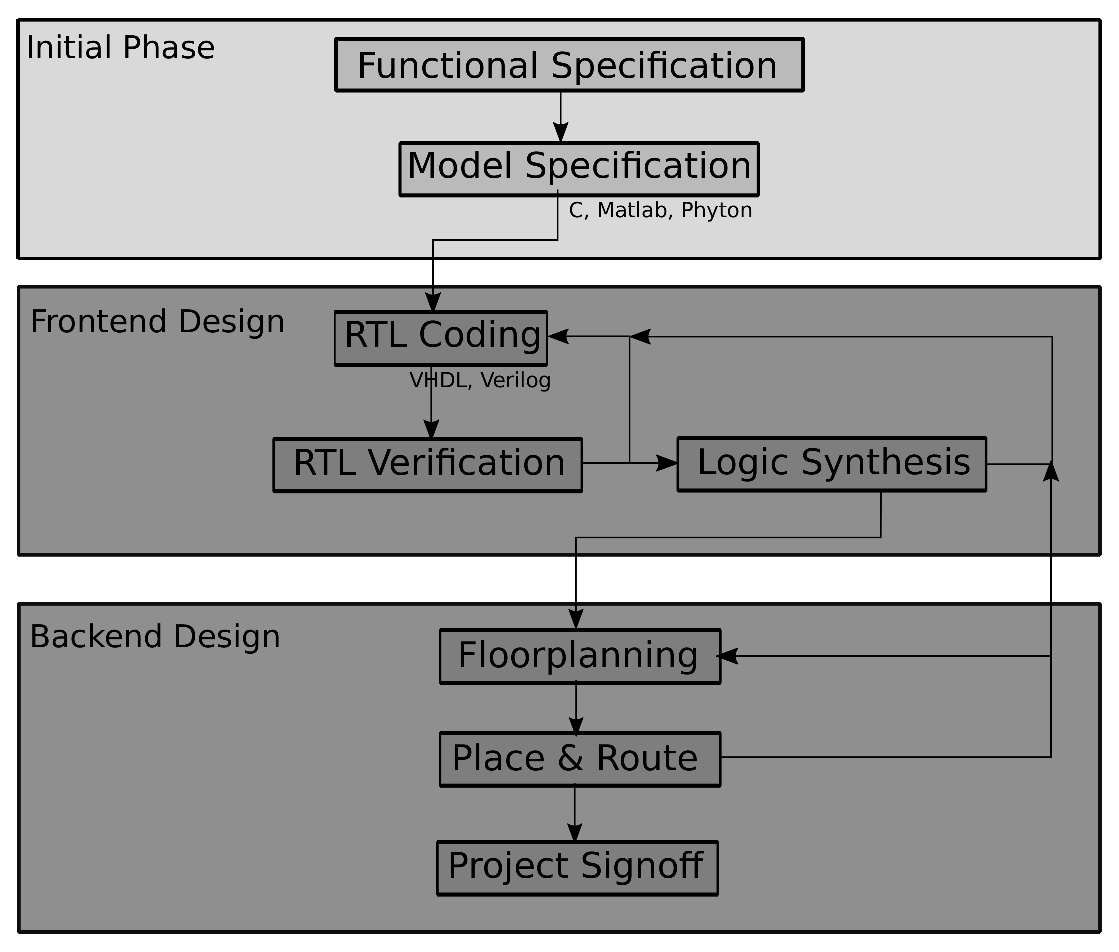
\includegraphics[width=0.6\textwidth]
      {./figures/asic_flow.eps}
%     \rule{35em}{0.5pt}
  \caption{ASIC design flow}
  \label{fig:asic_flow}
\end{figure}

%Once the requirements are defined the architecture is designed. The architecture implements the behavior of the previously defined blocks through boolean functions, finite state machines,
%combinatorial and sequential Logic. That description of the digital circuit is called the Register Transfer Level (RTL), the RTL description or architecture describes a digital circuit that performs complex computations, complex algorithms are described with logic gates, state machines combinational and sequencial logic, as and or gates, multiplexors, . Then, this RTL is described in a Hardware Description Language (HDL), a language developed for digital logic. This description in HDL language goes through a verification process, the behavior of the RTL must match that of the model. 
\section{Front-end}

Once the requirements are defined, the next step is to design the architecture of every block in the system. The architecture is a description of the digital circuit that must perform an intended tasks, also called of Register Transfer Level (RTL), the  digital circuit performs complex computations, protocol management or reorders data. The tasks are described with logic gates, state machines, combinational and sequential logic, \emph{and}, \emph{or} gates, multiplexors and flip flops. After the architecture is completely defined, an RTL description in a Hardware Description Language (HDL) is performed. HDLs describe the structure and behavior of the digital logic circuit, similar to a programming language, it achieves the description by means of a textual description consisting of expressions and statements. 

This RTL behavioral model then goes through a verification process, the behavioral RTL written in HDL language is simulated, and the results are compared with that of the high level language reference model. During the verification process, the circuit is stimulated with real data and timing and functional behavior is tested. The high level language model written in e.g. C, Matlab or Phyton, receives the same stimulus of the behavioral RTL model and generates a reference output. The two outputs are then compared and the RTL debugged if necessary, in case of differences with the reference. Time, behavioral and functional verification at this stage also allows for architectural exploration, optimal data widths (quantization levels) can be adjusted, for blocks involving fixed point computations, and performance issues can be identified.

Once the RTL is verified and no errors are present, Gate Level Synthesis is performed. This synthesis verifies if the HDL description can in fact be mapped to a specific digital hardware. Every logic that is described in the HDL language is mapped onto basic logic gates, \emph{and}, \emph{or} gates and lookup tables, memories and registers are also inferred from the RTL HDL description. Those primitives components are also known as standard cells. The gate level synthesis output is then, a description on a more low level stage. The netlist (the output at this stage) shows an entire structural description of the RTL design. At this stage rough, area, timing and power estimations can be performed, therefore if the goals of the design are not meet e.g. if the maximum frequency of operation defined was 20MHz and the circuit only achieves 15MHz, the behavioral description or even the architecture must be changed in order to attain the time/power/area requirements. 

%yielding estimates that can generate changes in the RTL design. There is a chance in almost all stages of the design, if the timing area or power goal are not reached withing that stage, that it may be necessary to go back to previous stages and modify the design. 

%FPGA prototyping is also performed at this stage, it allows to extend and strengthen ASIC functional verification. Although FPGAs prototypes performance is limited when compared to that of an ASIC, the logical functionality is the same. FPGAs allows for early integration in embedded software and a more realistic verification, since real stimulus can be applied to the design. Another reason to expend time prototyping in FPGA is total development costs, since FPGA prototypes increase the probability of getting the design bug-free in fewer tape-outs. 

FPGA prototyping is also performed at this stage, to extend the design verification. FPGA simulation time is faster than that of a PC allowing less simulation time. Moreover, FPGA prototyping allows for early integration in the embedded system and a more realistic verification, since real stimulus can be applied to the design. Another reason to expend time prototyping in FPGA is total development costs. FPGAs prototypes increase the probability of getting the design bug-free in fewer tape-outs. 

%Although FPGAs prototypes performance is limited when compared to that of an ASIC, the logical functionality is the same. Also, 

\section{Back-end}

Once the frontend bug-free netlist if generated a physical implementation is performed. Basically the process follows three key steps: 

\begin{itemize}
\item \emph{Floor Planing} In Floorplaning the subblocks that compose the design are strategically distributed on the chip area. Blocks are placed in such a way that noise between components is avoided, reduction in timing paths is also 
accomplished and power distribution of the chip is planed.

\item \emph{Placement} The placement process maps the logic with the standard cells and tries to adjust all the cells 
within the chip area to that of the restrictions defined in the floorplaning. The placement process also maps the standard cells to the actual technology used, the pre-designed cells are provided by the foundry (the semiconductor fabrication facility) chosen to manufacture the chip. 

\item \emph{Routing}: Finally the routing process uses the information on the netlist to connect the standard cells one with another. The placement and routing process are iterative, they go back and forth until the process is completed. 

\end{itemize}


After the routing process is complete and timing, function and power requirements are checked, a physical verification is performed. A series of tests are performed on the final circuit: the design rule check (DRC) test some design rules imposed by the foundry, so that the chip can perform as expected. Also, the layout versus schematic (LVS) simulation and an electric rule check (ERC) is performed on the physical verification. 

There is a chance in almost all stages of the ASIC design flow  (if the timing, area or power goals are not reached withing that stage) that it may be necessary to go back to previous stages and modify the design, architecture, RTL (even algorithms can change) if in the final stages the design does not reach the desired results. 

%1. Speed
%2. Area
%3. Power
  \chapter{The Discrete Fourier Transform and Fast Fourier Transform}
Frequency domain analysis is widely used in the DSP area, a signal in time domain is transformed to frequency domain by means of the DFT. Since the direct implementation of the DFT is time consuming and due to the widely range of applications of the DFT, several algorithms called of Fast Fourier Transforms originated. Fast Fourier algorithms decrease the DFT complexity (fewer operations and/or simpler computations tasks) by means of a divide and conquer approach. Essentially it maps the problem into several sub-problems and applies the division recursively to the sub-problems as well, eventually leading to a reduction in computation complexity. 

Fast algorithms can be classified in two major classes, those based on the Good's mapping, which basically factors the DFT or divides the DFT into smaller DFTs with its sizes being co-prime, this approach has the advantage of no producing any Twiddle Factor (equation \ref{eq:twiddle}), with this a lower bound in complex multiplications is achieved, the Winograd Fourier Transform (\ac{wfta})~\cite{winograd1978computing} and Prime Factor algorithm (\ac{pfa})~\cite{pfa_fft} are two of the algorithms based on this method. A second class of algorithms known as Cooley-Tukey Fast Fourier Transform (\ac{ctfft}) or radix-r algorithms, suitable for $r^n$ size sequences, where the use of twiddle factors is inevitable.

CTFFT algorithms adds regularity to the computation, considering that CTFFT algorithms show a more repetitive use of fewer modules, and are easier to implement in a parallel kind of way, since the small repetitive modules are applied on contiguous sets of data. This also is advantageous since improvements in those small repetitive blocks allows from an overall improvements of the computation. Moreover, CTFFT algorithms are more suitable for in-place computation, a desired feature since no additional memory is required. On the other hand, algorithms like the WTFA requires huge memory and does not allow for in-place computation~\cite{duhamel1990fast}. 


All the advantages of the CTFFT algorithms over Good's based ones, lead to Cooley-Tukey algorithms begin more used in implementations. Complex multiplications alone are not the main concern in implementation and computation time, number of additions, memory access, communications costs are examples of other variables that are at least as important. It is worth noticing that while a lot of research have been done in the subject due to the importance of the DFT and FFT algorithms, new algorithms continue to emerge as is the case of the Sparse Fourier Transform presented in \cite{sfft_paper} and implemented in \cite{milion_point_sfft} for a million point DFT. This algorithms takes advantage of the sparsity shown in some signal where the DFT is applied, that is, only a phew components of the signal are of importance since all other signal components in frequency domain are zero, the algorithm then only computes the set of needed non-zero frequency components. This is not the case of the current intended application, therefore, the classic approach to the FFT implementation is adopted. In the following, a review of the Cooley-Tukey approach to the DFT computation is presented.




\section{FFT Cooley-Tukey Algorithm}




The DFT is a mathematical tool widely used in signal processing. Basically, the DFT of a \textit{N}-point sequence converts discrete samples from time-domain to frequency-domain and vice versa through equation \ref{eq:dft}: 

 \begin{equation} 
     X[k]=\sum _{n=0}^{N-1} x[n]W^{nk}_N,
     \label{eq:dft}
 \end{equation}
where $k =0,1,2,\cdots,\textit{N}-1$ and $W_N$ (also known as twiddle factor)
is given by:
 \begin{equation} 
     W_N= \textit{e}^{\frac{-j2\pi}{N}}.
     \label{eq:twiddle}
 \end{equation}
An \textit{N}-point inverse DFT (IDFT) is computed as: 
 \begin{equation} 
     x[n]=\frac{1}{N}\sum _{k=0}^{N-1} X[k]W^{-nk}_N.
     \label{eq:idft}
 \end{equation}

The direct computation of the DFT is difficult to implement due to its high computation complexity, for instance, a $N$ points computation of a sequence composed of complex samples requires $N^2$ complex multiplications (each complex multiplication is equal to $4$ real multiplications and $2$ real additions) and $N^2-N$ complex additions (every complex addition is equal to $2$ real additions), a complexity of $O(N^2)$~\cite{proakis1996digital}. 

% Based on the symmetry(eq \ref{eq:twidle_sym}) and periodicity  (eq \ref{eq:twidle_period}) property of the twiddle factor and a divide-and-conquer approach a new class of algorithms that optimizes the computation of the DFT were developed \cite{cooley_fft}, this new class of algorithms are known as Fast Fourier Transform (FFT). The Cooley and Turkey algorithm is a well known FFT algorithm, in the next section a description of the algorithm is presented.


%  \begin{equation} 
%      \centerline{Symmetry: ${W}_{N}^{k+N/2} = -{W}_{N}^{k}$}
%      \label{eq:twidle_sym}
%  \end{equation}


% \begin{equation} 
% \centerline{Periodicity: ${W}_{N}^{k+N} = {W}_{N}^{k}$}
% \label{eq:twidle_period}
% \end{equation}

Based on a divide-and-conquer approach a new class of algorithms that optimizes the computation of the DFT were developed, this new class of algorithms are known as Fast Fourier Transform (FFT). The Cooley and Turkey\cite{cooley_1965} algorithm is a well known FFT algorithm.

The divide and conquer approach divides the computation problem in smaller problems, and solves every smaller problem recursively using the same algorithm, the solution to the original problem is then the combination of the smaller solutions. A common approach is to divide the problem by half, then each half is then divided by half, and so on. This is known as radix-2 FFT, the partition goes until only size two DFTs remain. Following this approach two type of FFTs are derived according to the domain where the division is performed, the Decimation in Time (DIT), where the partition occurs on the input sequence (time domain), and the Decimation in Frequency (DIF) where the output sequence is partitioned (frequency domain). 

%Two kinds of FFT algorithms are found in the literature, a decimation in time FFT, which divides the input sequence into even and odds samples iteratively until only size $2$ DFTs are computed, and the decimation in frequency which uses a similar approach, only that in this case the decimation is performed over the frequency samples. When the decimation is performed in pairs it is called Radix-2, higher radixes FFTs are also used, where only size $r$ ($r$ beign an integer multiple of $2$) DFTs are computed after the decimation process, either in time or frequency domain.       

The decimation in frequency algorithm is derived as follows,  given a $x(n)$ sequence of length $N = 2^p$, where $p$ is an integer, the DFT of a time sequence $x(n)$ computed as in eq.~\ref{eq:dft} can be written as:

\begin{equation} 
\begin{split}
     X[k]=\sum _{n=0}^{N/2-1} x[n]W^{nk}_N + \sum _{n=N/2}^{N} x[n]W^{nk}_N  \\  =\sum _{n=0}^{N/2-1} x[n]W^{nk}_N + W^{Nk/2}_N\sum _{n=0}^{N/2-1} x[n+N/2]W^{nk}_N,
     \label{eq:dft2}
     \end{split}
\end{equation}

% \begin{multline} 
%      X[k]=\sum _{n=0}^{N/2-1} x[n]W^{nk}_N + \sum _{n=N/2}^{N} x[n]W^{nk}_N  \\  =\sum _{n=0}^{N/2-1} x[n]W^{nk}_N + W^{nk/2}_N\sum _{n=0}^{N/2-1} x[n+N/2]W^{nk}_N,
% \end{multline}
 Since ${W}_{N}^{Nk/2} = (-1)^k$ eq.~\ref{eq:dft2} can be written as:

\begin{equation} 
     X[k]=\sum _{n=0}^{N/2-1} [x(n) + (-1^{k})x(n+N/2)]W^{nk}_{N}
\label{eq:dft_even}
\end{equation}

Decimating in frequency (i.e. splitting in odds and even frequency components) and using the fact that ${W}_{N}^{2} = {W}_{N/2}^{}$, 


\begin{equation} 
     X[2k]=\sum _{n=0}^{N/2-1} [x(n) + x(n+N/2)]W^{nk}_{N/2}
\label{eq:dft_even}
\end{equation}


\begin{equation} 
     X[2k +1]=\sum _{n=0}^{N/2-1} [[x(n) - x(n+N/2)]W^{n}_{N}]W^{nk}_{N/2}
\label{eq:dft_odd}
\end{equation}


The entire coputation of the $N/2$ point sequences \ref{eq:dft_even} and \ref{eq:dft_odd} can be rewritten as: 

\begin{equation} 
     X[2k]=\sum _{n=0}^{N/2-1} g1(n)W^{nk}_{N/2}
\label{eq:dft_even2}
\end{equation}

\begin{equation} 
     X[2k+1]=\sum _{n=0}^{N/2-1} g2(n)W^{nk}_{N/2}
\label{eq:dft_odd2}
\end{equation}

where 

\begin{equation} 
  g1(n) = [x(n) + x(N/2 + n)]
\label{eq:dft_btfly1}
\end{equation}

\begin{equation} 
    g2(n) = [x(n) - x(N/2 + n)]W^{nk}_{N/2}
\label{eq:dft_btfly2}
\end{equation}

Fig.~\ref{fig:dif_1}, shows an example of the computation of eq.~\ref{eq:dft_odd} and \ref{eq:dft_even} for a 8 point sequence. It can be seen as two DFTs of half the sequence size, with two input sequences given by eq.~\ref{eq:dft_btfly1} and eq.~\ref{eq:dft_btfly2}.

\begin{figure}[htbp]
  \centering
   \includegraphics[width=0.4\textwidth]{./figures/fft_partial_dif}
    %\rule{35em}{0.5pt}
  \caption{First stage in the DIF computation process}
  \label{fig:dif_1}
\end{figure}

Performing the same computations on the $N/2$ point DFTs until only remains two points DFTs, an optimization in the algorithm can be made. Fig.~\ref{fig:dif_diagram} shows a diagram of the entire computation process for a DFT of size 8 using the FFT. It can be seen highlighted the basic computation process performed in every stage, two complex samples are added, subtracted and multiplied by the twiddle factor. This operation is known as the butterfly (fig. \ref{fig:DIF_btfly}), and it involves one complex multiplication and two complex additions.    

\begin{figure}[htbp]
  \centering
   \includegraphics[width=0.6\textwidth]{./figures/btfly}
    %\rule{35em}{0.5pt}
  \caption{Decimation in frequency butterfly}
  \label{fig:DIF_btfly}
\end{figure}

There are $N/2$ butterflies per stage and $log2(N)$ stages. Thus,  the total number of complex multiplications is $N/2log2(N)$ and complex additions is $Nlog(N)$ which is much less than $N^2$ complex multiplications and $N^2-N$ complex additions of the direct implementation, this algorithm shows a complexity of $O(N/2log2(N))$. The optimization of the algorithms relies on the redundancy present on the twiddle factor which is exploited consequently using less multiplications to perform the computation. Higher radices (4, 8, 16) can be derived when the division of the sequence done by $2^n$ $n = 1, 2, 3, 4, .. etc$. Fewer multiplications at the cost of a more complex butterfly and control of the entire computations is achieved with higher radices.  In the next section the implications of the hardware implementation of the FFT algorithm is addressed. 

\begin{figure}[htbp]
  \centering
   \includegraphics[width=1\textwidth]{./figures/DIF_FFT.pdf}
    %\rule{35em}{0.5pt}
  \caption{Decimation in frequency diagram}
  \label{fig:dif_diagram}
\end{figure}


  \chapter{Architecture of the Fast Fourier Transform}

\section{Proposed Architecture}
\label{sec:proposed_fft_architecture}


%\subsection{Overview}

Typically two kinds of hardware implementations are adopted to compute the FFT; namely the ``in-place'' and pipeline or parallel approach~\cite{chu2000inside}. The ``in-place'' approach performs a single computation per clock, thus a single computation unit(a Butterfly unit) and a $N$ size memory is used. Basically the butterfly reads data from the memory, performs the computation and writes the results back to the same memory space from were it read the data. This kind of implementation has low hardware cost, since it reuses the computation unit and other hardware resources. However, with this approach the throughput is relative low, since it can perform only one butterfly operation per cycle. In the pipeline approach~\cite{mitvlsi} several butterfly units perform the computation in parallel, typically one butterfly for every FFT stage. This approach uses more resources, but the throughput is much higher than that of ``in-place'' architectures. 

\subsection{FFT Implementation}

\subsubsection{Hardware Considerations}

The architecture presented is a collection of methods and algorithms that are believed to simplify the complexity of the FFT hardware implementation. The architecture chosen to achieve the standard requirements for the DFT implementation is based on the ``in-place'' approach. As was mentioned before this method has low throughput, yet consumes less hardware when compared with parallel architecture, as needed by the IEEE802.15.4g standard.

The  ``in-place'' method also allows more hardware reuse if the architecture is intended for variable size FFTs. The same hardware is used to perform the computation, varying only the time spent to do so. This could not be accomplished by an pipeline architecture, since one butterfly and a memory module is needed per FFT stage, leaving resources unused for the lower size FFTs, wasting power. In the following a description of the various parts that compose the FFT/IFFT architecture is presented. 

%increasing the static power consumption.

\paragraph{Memories}

The ``in-place'' FFT computation consists in taking two data samples from memory, perform the computations
and write back the computed values to memory, the process is repeated $N/2log_{2}(N)$ times. To take advantage of parallelism two banks of double-port memory are used, namely M0 and M1, allowing the butterfly unit to retrieve two data points simultaneously, as well as to write data to memory in the same manner. 

\paragraph{Address Generator (ADG)}
\label{sec:address_generator}

%If data is read from different memory banks and written to different memory banks an in-place approach can be  reached

In the ``in-place'' approach scheme the computed data is written back to the memory space from where it was read. In the ordinary flow of the algorithm this only occurs in the first stage of the FFT (See FFT Diagram in Fig.~\ref{fig:fft_dia_memories}), e.g  taking samples $X[0]$ from M0 and $X[4]$ from M1, computing the butterfly (B1 in the example of figure \ref{fig:fft_dia_memories}) and write the result back in different memory banks. In~\cite{xiao_2007}, Xiao proposed an in-place addressing method that uses 
reduced logic achieving an ``in-place'' approach where data is read/written from difference memory banks in parallel Basically, Xiao's approach exchanges data at the input/output of the butterfly. Addresses are generated according to the data exchanged achieving an ``in-place'' memory read/write scheme.   
The address generation consists of two main counters, 
\textit{CountB} and \textit{CountS}. The former for the butterfly being 
computed and the later for the stage that is currently in progress, according to Fig.\ref{fig:dif_diagram}.

\begin{figure}[htbp]
\centering
\includegraphics[width=0.7\textwidth]{./figures/arch_addr.pdf}
\caption{Address Generator}
\label{fig:Addr_gen}
\end{figure} 


The number of butterflies/stages being computed depends on the MR-OFDM mode that is currently set. For an $N$-sized FFT, $log_{2}(N)$ stages and $N/2$ butterflies are required. Since the MR-OFDM FFT/IFFT supports different FFT sizes the counters are chosen to support the maximum possible size ($N$=128). Once the butterfly counter has reached the appropriate value, a reset is applied and the stage counter is incremented. To accomplish the variable FFT size some constant values are set according to the chosen OFDM option, those constants are used to compare the current butterfly and stage count and reset the counters. The ``in-place''  approach has some advantages over the pipeline implementations of the FFT, the hardware reuse of the ``in-place'' approach is almost total, the same hardware is used for the various FFT sizes needed by the MR-OFDM.  

% 
\begin{figure}[htbp]
\centering
\includegraphics[width=0.8\textwidth]{./figures/Butfly_DIf_RAMs}
\caption{8 point FFT DIF diagram}
\label{fig:fft_dia_memories}
\end{figure} 


The address generation logic is as follows, the addresses for the first memory bank (M0) is taken directly from the butterfly counter, as it increases so does the address. The address for the second memory bank M1 changes with the stage that is 
currently being computed, the value
of \textit{CountS} determines the amount of bits from \textit{CountB} that
are inverted in a big-endian mode. This is accomplished by a series of 2:1 
multiplexers, one for every address bit. 
The multiplexers are controlled by a $B$-sized shift register that shifts one bit at each stage, its inputs are the value of \textit{CountB} and inverted \textit{CountB}. Additionally exchange multiplexers are placed at the input/output of the butterfly. These exchange multiplexers alternate the butterfly input/output to the memories being read/written. The multiplexers control signals are generated according to the butterfly (\textit{CountB}) and state counter (\textit{CountS}). 
For computing a FFT of size $N = 2^n$, $log_2(N)$ stages and $N/2$ 
butterflies per stage are needed. Thus, the address generator 
needs \textit{CountS} and \textit{CountB} with $(n-1)$bits and $\lceil log_2(n) \rceil$bits, respectively. Fig.~\ref{fig:Addr_gen} shows a simple FFT architecture with the blocks involved in the address generation highlighted.

\paragraph{Butterfly Unit}

The basic computation performed at every FFT stage is the butterfly computation. Fig.~\ref{fig:DIF_btfly} shows the  butterfly diagram for a Radix-2 decimation in frequency FFT.  The operation involves taking two data samples, performing the addition and subtraction between each one, and multiplying the subtraction result by the twiddle factor(eq.~\ref{eq:twiddle}).

The complex multiplication, in its purest form (without any optimization \cite{bib:chu_black_box})  requires four real multiplications and two real additions/subtractions, an operation that is usually very large and time consuming. The Coordinate Rotation Digital Computer (CORDIC) 
algorithm~\cite{voider1959} is an alternative to perform the complex multiplication operation, it requires only
add and shift operations, figure~\ref{fig:btfly_arch} shows the detailed architecture of the DIF butterfly. The CORDIC algorithm is detailed in section~\ref{section:CORDIC}.

\begin{figure}[htb!]
\centering
\includegraphics[width=0.8\textwidth]{./figures/butterfly_architecture.pdf}
\vspace{-0.2 cm}
\caption{DIF Butterfly Architecture}
\label{fig:btfly_arch}
\end{figure}

%The twiddle factor is usually precomputed and stored in a ROM memory. 

Additionally, using the CORDIC to perform the complex multiplication, the ROM memory usually implemented to store the twiddle factor can be eliminated~\cite{Kuo2003}\cite{Oruklu2012}. The substitution of the complex multiplier is as follows, the twiddle factor multiplication is equivalent to the rotation of the sequence $x(n)$ by an angle 
$-\frac{2\pi}{N}nk$, operation that can be performed by the CORDIC algorithm. Although, the 
substitution of the multiplier by the CORDIC algorithm in the butterfly unit avoids the need
of a memory to store twiddle factors values a ROM memory would still be needed to store the phase
angles. However, if the order in which the data is read follows a pattern in the phase angles they can be generated in a generic way, as is the case of the addressing scheme presented in the previous section. 

%Table \ref{table:16_FFT_angles} shows the angles values for a 16 point FFT in each stages. Here
%we see a pattern in the angle values, the non-zero values are always equal to $\pi/(N/2)$ 
%multiplied by an integer. It can be noticed from the bit representation of this integer 
%(table\ref{table:16_FFT_angles_bin} ) that the next stage value is equal to the previous 
%one shifted in one bit, or the first value shifted $S$ times, where $S$ is the number of 
%the $n^{th}$ stage. Therefore, this integer value can be generated by taking the butterfly
%counter and shifting its value at every stage. Then, the angle can be obtained  by 
%multiplying this value with the constant $\pi/(N/2)$ value.

Table \ref{table:16_FFT_angles} shows the angles values for a 16 point FFT in each stages. Here
the angle values shows a pattern, the non-zero values are always equal to $\pi/(N/2)$ 
multiplied by an integer. It can be noticed from the bit representation of this integer 
(table\ref{table:16_FFT_angles_bin} ) that the next stage value is equal to the previous 
one shifted in one bit, or the first value shifted $S$ times, where $S$ is the number of 
the $n^{th}$ stage. Therefore, this integer value can be generated by taking the butterfly
counter and shifting its value at every stage. Then, the angle can be obtained  by 
multiplying this value with the constant $\pi/(N/2)$ value.


\begin{table}[h]
\parbox{.45\linewidth}{
\centering
\vspace{0.5cm}
\caption{Angle values for a 16 size FFT}
    \label{table:16_FFT_angles}
\begin{tabular}{@{}c c c c c c}
\hline
Stage 0  & Stage 1  & Stage 2  & Stage 3 \\ \hline
0        & 0        & 0        & 0       \\ 
$1\pi/8$ & $2\pi/8$ & $4\pi/8$ & 0       \\ 
$2\pi/8$ & $4\pi/8$ & 0        & 0       \\ 
$3\pi/8$ & $6\pi/8$ & $4\pi/8$ & 0       \\ 
$4\pi/8$ & 0        & 0        & 0       \\ 
$5\pi/8$ & $2\pi/8$ & $4\pi/8$ & 0       \\ 
$6\pi/8$ & $4\pi/8$ & 0        & 0       \\ 
$7\pi/8$ & $6\pi/8$ & $4\pi/8$ & 0       \\ \hline

\end{tabular}

}
\hfill
\parbox{.45\linewidth}{
\centering
\caption{Bit representation of Counter B shifted for a 16 point FFT}
    \label{table:16_FFT_angles_bin}
\begin{tabular}{@{}c c c c c c}
\hline
Stage 0 & Stage 1 & Stage 2 & Stage 3 \\ \hline
000     & 000     & 000     & 000     \\ 
001     & 010     & 100     & 000     \\ 
010     & 100     & 000     & 000     \\
011     & 110     & 100     & 000     \\ 
100     & 000     & 000     & 000     \\ 
101     & 010     & 100     & 000     \\ 
110     & 100     & 000     & 000     \\ 
111     & 110     & 100     & 000     \\ \hline
\end{tabular}
    

}
\end{table}


\subsubsection{CORDIC}
\label{section:CORDIC}
The CORDIC~\cite{voider1959} is an algorithm that allows the implementation of many trigonometric functions using basic arithmetic, (subtraction, addition and shifts), this is ideal for hardware implementation since trigonometric functions are resource consuming. The CORDIC algorithms emerges from a simplification of the rotation of a vector, it is as follows:

\begin{figure}[!h]
\centering
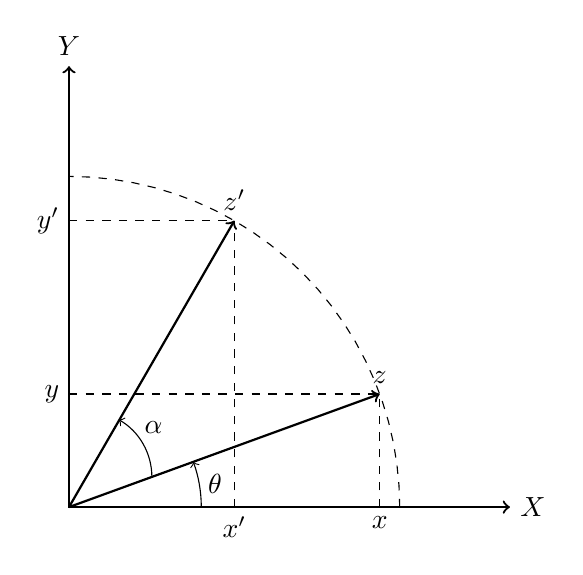
\begin{tikzpicture}[scale=2.8]
    % Draw axes
    \draw [<->,thick] (0,2) node (yaxis) [above] {$Y$}
        |- (2,0) node (xaxis) [right] {$X$};
    % Draw two intersecting lines
    
    
    \draw [->,thick] (0,0) coordinate (a_1) -- ({1.5*cos(20)}, {1.5*sin(20)}) coordinate (a_2) node[black, above] {$z$} ;
    \draw [->,thick] (0,0) coordinate       -- ({1.5*cos(60)}, {1.5*sin(60)}) coordinate (a_4) node[black, above] {$z'$};   
    
    %\draw pic["$\alpha$", draw=orange, ->, angle eccentricity=1.2, angle radius=1cm] {angle=b--a--c};
    
    %%NODES
%     \draw  (0,0) 		     coordinate (a) node[] {ORIGEN};
%     \draw  ({1.5*cos(20)},0) coordinate (b) node[] {P1};
%     \draw  ({1.5*cos(20)},{1.5*sin(20)}) coordinate (c) node[] {P2};
    
    
    \draw [->] (0.6,0) arc (0:20:0.6) node[pos=0.5, xshift=0.2cm] {$\theta$};
    \draw [->] ({0.4*cos(20)},{0.4*sin(20)}) arc (0:60:0.3) node[pos=0.8, xshift=0.3cm] {$\alpha$};
   % \pic [draw, ->, "$\theta$", angle eccentricity=1.5] { angle = a_1--a_2--a_4 };
    %\draw (0,1.5) coordinate (b_1) -- (2.5,0) coordinate (b_2);
    % Calculate the intersection of the lines a_1 -- a_2 and b_1 -- b_2
    % and store the coordinate in c.
    %\coordinate (c) at (intersection of a_1--a_2 and b_1--b_2);
    
    \draw [dashed,domain=0:90] plot ({1.5*cos(\x)}, {1.5*sin(\x)});
    
    \draw [dashed] (0, {1.5*sin(20)}) node[left] {$y$} -- ({1.5*cos(20)}, {1.5*sin(20)}) ;
    \draw [dashed] ({1.5*cos(20)}, 0) node[below]{$x$} -- ({1.5*cos(20)}, {1.5*sin(20)}) ;
    
    \draw [dashed] (0, {1.5*sin(60)}) node[left] {$y'$} -- ({1.5*cos(60)}, {1.5*sin(60)});
    \draw [dashed] ({1.5*cos(60)}, 0) node[below] {$x'$} -- ({1.5*cos(60)}, {1.5*sin(60)});
    
    % Draw lines indicating intersection with y and x axis. Here we use
    % the perpendicular coordinate system
    
    %\draw[dashed] (yaxis |- c ) node[left] {$y'$}
    %    -| (xaxis -| c) node[below] {$x'$};
    
    % Draw a dot to indicate intersection point
    %\fill[red] (a_2) circle (2pt);
\end{tikzpicture}
\caption{Rotation of a vector}
\label{fig:cdc_rotation_vector}
\end{figure}
% The CORDIC~\cite{voider1959} algorithm is an iterative technique based on the rotation of a vector which allows many  trigonometric functions to be calculated. The advantage of this method is that it is accomplished using only shifts and
% adds, which are easier to implement in hardware. In the Following, an overview of the algorithm is presented:

The rotation of a vector of magnitude $||z||$ from position $z$ to position $z'$ is given by equations eq.~\ref{eq:rotate_vector_x} and eq.~\ref{eq:rotate_vector_y}:

\begin{equation} 
\begin{gathered}
x^{'} = \Vert{z}\Vert (cos(\alpha)cos(\theta) - sin(\alpha)sin(\theta)) \\
x^{'} = xcos(\theta) - ysin(\theta)      
    \label{eq:rotate_vector_x}
\end{gathered}
\end{equation}

\begin{equation} 
\begin{gathered}
y^{'} = \Vert{z}\Vert (sin(\alpha)cos(\theta) + cos(\alpha)sin(\theta)) \\
y^{'} = ycos(\theta) + xsin(\theta)      
	\label{eq:rotate_vector_y}
\end{gathered}
\end{equation}

That can be expressed as

\begin{equation} 
x^{'} = cos(\theta)(x - ytan(\theta))
    \label{eq:rotate_vector_x2}
\end{equation}

\begin{equation} 
y^{'} = cos(\theta)(y + xtan(\theta))
	\label{eq:rotate_vector_y2}
\end{equation}

Removing the $cos(\theta)$ term to simplify the operation, the rotation becomes a pseudo rotation

\begin{equation} 
x^{'} = x - ytan(\theta)
    \label{eq:pseudo_rotate_x}
\end{equation}

\begin{equation} 
y^{'} = y + xtan(\theta)
	\label{eq:pseudo_rotate_y}
\end{equation}

The pseudo rotation by an angle $\theta$ can be achieved by successive smaller rotations. Restricting the angles so that every smaller rotation becomes $tan(\theta)^i = 2^{-i}$, the pseudo-rotation or the multiplication by $tan(\theta)$ becomes a multiplication by $2^{-i}$, which can be implemented in hardware by simply shifting a binary string. Thus, rotating an input vector by an angle $\theta$ is now an iterative process made-up of successively shifts and adds operations. 

 \begin{equation} 
x^{i+1} = x(i) - d_i(2^{-i}y(i))
    \label{eq:cordic_x}
\end{equation}

\begin{equation} 
y^{i+1} = y(i) + d_i(2^{-i}x(i))
	\label{eq:cordic_y}
\end{equation}

\begin{equation} 
z^{i+1} = z^{i} - d_i arctan 2^{-i}
    \label{eq:cordic_z}
\end{equation}

\begin{equation} 
 d_i = \begin{Bmatrix}
      -1 & if \quad z_i  < 0  \\
      +1 & if \quad z_i  > 0 
       \end{Bmatrix}
   \label{eq:cordic_d}
   \end{equation}

Equations \ref{eq:cordic_x}, \ref{eq:cordic_y}, \ref{eq:cordic_z} describe the CORDIC algorithm, the third equation(eq.~\ref{eq:cordic_z}) is called the angle accumulator and in conjunction with $d_i$ eq.~\ref{eq:cordic_d} (known as the decision operator) determines the direction of the rotation. The operation mode shown is known as the Rotation mode~\cite{voider1959} and it rotates the input vector by an specified angle, the angle accumulator is initialized with the desired rotation angle and for every iteration the decision operator is chosen such that the magnitude of the residual angle tends to zero. The decision operator is then determined by the sign of the angle accumulator.  
%The presented mode of the CORDIC is known as the rotation mode, where the input vector is rotated by an specified angle given as an input ($z_0$). 
%$d_i$ (eq.~\ref{eq:cordic_d}) is the decision operator and it is used to determine in which direction to rotate. 

Since the $cos(\theta)$ term is removed to simplify the algorithm the outputs $x$ and $y$ are scaled by a factor $k_n$, the scaling factor is given by:

%
\begin{equation} 
\begin{gathered}
k_n = \prod_{i=1}^{n} \frac{1}{cos(\theta)^{i}} = \prod_{i=1}^{n} \sqrt{1+tan^2\theta^{i}} =  \prod_{i=1}^{n} \sqrt{1+2^{-2i}}\\
k_n \rightarrow 1.6476 \textrm{ as n} \rightarrow \infty
    \label{eq:cordic_kn}
\end{gathered}
\end{equation}


After $n$ iterations the CORDIC output is given by:


\begin{equation} 
\begin{gathered}
x_{n} = k_n [x_{0} cos(z_{0}) - y_{0} sin(z_{0})]
    \label{eq:cordic_rotation_x}
\end{gathered}
\end{equation}

\begin{equation} 
\begin{gathered}
y_{n} = k_n [y_{0} cos(z_{0}) + x_{0} sin(z_{0})]
    \label{eq:cordic_rotation_y}
\end{gathered}
\end{equation}

\begin{equation} 
\begin{gathered}
z_{n} = 0
    \label{eq:cordic_rotation_z}
\end{gathered}
\end{equation}

A second operation mode called Vectoring mode can be accomplished if instead of $d_{i} = sign(z_{i})$, is chosen such that $d_{i} = sign(y_{i})$. In this mode the vector is rotated by the necessary angle so that the $x$ component of the result vector is maximized and its $y$ component tends to zero. After $n$ iterations the CORDIC output in Vectoring mode is given by:


\begin{equation} 
\begin{gathered}
x_{n} = k_n \sqrt[]{x_0^2 + y_0^2} 
    \label{eq:cordic_vectoring_x}
\end{gathered}
\end{equation}

\begin{equation} 
\begin{gathered}
y_{n} = 0
    \label{eq:cordic_vectoring_y}
\end{gathered}
\end{equation}

\begin{equation} 
\begin{gathered}
z_n = z_0+\tan^{-1}(y_0/x_0)
    \label{eq:cordic_vectoring_z}
\end{gathered}
\end{equation}

The CORDIC equations (eq.~\ref{eq:cordic_x},~\ref{eq:cordic_y},~\ref{eq:cordic_z}) can be adapted to perform operations in other coordinate systems, namely circular, hyperbolic and linear~\cite{cordic_tiago}. A new variable $m$, defines the coordinate system used. Equations~\ref{eq:cordic2_x},~\ref{eq:cordic2_y},~\ref{eq:cordic2_z} define the new generalized CORDIC equations, table~\ref{table:cordic_modes} shows the operation modes. In table~\ref{table:cordic_gen} the CORDIC  outputs  for the three modes of operation are shown and finally table~\ref{table:cordic_func} shows some of the functions that can be computed with the CORDIC algorithm. 


\begin{equation} 
x_{i+1} = x(i) - m d_i[2^{-i}y(i)]
    \label{eq:cordic2_x}
\end{equation}

\begin{equation} 
y_{i+1} = y(i) + d_i[2^{-i}x(i)]
	\label{eq:cordic2_y}
\end{equation}

\begin{equation} 
z_{i+1} = z^{i} - d_i\sigma_{i}
    \label{eq:cordic2_z}
\end{equation}

\begin{table}[h]
\centering
\caption{CORDIC Modes of operation}
\label{table:cordic_modes}
\begin{tabular}{ccccc}
\hline
Mode      & $d_{i}$       & Coordinate System & $\sigma_{i}$  & m  \\ \hline
Vectoring & $sign(y_{i})$ & Circular          & $tan(2^{-i})$ & 1  \\
Rotation  & $sign(z_{i})$ & Hiperbolic        & $tanh(2^-i)$  & -1 \\
-         &               & Linear            & $2^-i$        & 0 \\ \hline
\end{tabular}
\end{table}


\begin{table}[h]
\centering
\caption{Results of CORDIC Generalized equations}
\label{table:cordic_gen}
\begin{tabular}{ccc}
\hline
\multicolumn{1}{c}{m}                  & Rotation Mode                                 & Vectoring Mode                           \\ \hline
\multicolumn{1}{c}{\multirow{3}{*}{1}} & $x_n = k_n[x_0 \cos(z_0) - y_0 \sin(z_0)]$   &  $x_n = k_n\sqrt{x_0^2 + y_0^2}$\\
\multicolumn{1}{c}{}                   & $y_n = k_n[y_0 \cos(z_0) + y_0 \sin(z_0)]$   & $y_n = 0$                                \\
\multicolumn{1}{c}{}                   & $z_n = 0$                                     & $z_n = z_0+\tan^{-1}(y_0/x_0)$    \\ \hline
\multirow{3}{*}{0}                     & $x_{n} = x_0$                                 & $x_n = x_0$                              \\
                                       & $y_n = y_0 + x_0 z_0$                         & $y_n = 0$                                \\
                                       & $z_0 = 0$                                     & $z_n = z_0 + (y_0 /x_0 )$                \\ \hline
\multirow{3}{*}{-1}                    & $x_n = k_h[x_0 \cosh(z_0) - y_0 \sinh(z_0)]$  & $x_n = k_h\sqrt{x_0^2 - y_0^2}$         \\
                                       & $y_n = k_h[y_0 \cosh(z_0) + y_0 \sinh(z_0)]$  & $y_n = 0$                                \\
                                       & $z_n = 0$                                     &       \\ \hline
\end{tabular}
\end{table}

\begin{table}[h]
\centering
\caption{Some Functions Computed by the CORDIC}
\label{table:cordic_func}
\begin{tabular}{crcccll}
\hline
Mode      & m  & $x_0$          & $y_0$          & $z_0$   & $x_n$                               & $y_n$ or $z_n$                           \\ \hline
Rotation  & $1 $ & $ k_n         $ & $0            $ & $ \theta $ & $ \cos(\theta)                       $ & $y_n = \sin(\theta)                   $ \\
Vectoring & $1 $ & $ 1            $ & $a            $ & $ 0      $ & $ k_n\sqrt{a^2+1} 		  $ & $ y_n = \tan^{-1}(a)$ \\
Rotation  & $-1$ & $ k_h         $ & $0            $ & $ \theta $ & $ \cosh{\theta}                    $ & $y_n = \sinh(\theta)                  $ \\
Rotation  & $-1$ & $ a            $ & $a            $ & $ \theta $ & $ k_nae^{\theta}  		  $ & $y_n = Kae^{\theta} $ \\
Vectoring & $-1$ & $ a            $ & $1            $ & $ 0      $ & $ k_n\sqrt{a^2-1} 		  $ & $z_n= \cot^{-1} (a) $ \\
Vectoring & $-1$ & $ a+1          $ & $a-1          $ & $ 0      $ & $ 2k_h\sqrt{a}                    $ & $z_n = 0.5\ln(a)                      $ \\
Vectoring & $-1$ & $ a+b          $ & $a-b          $ & $ 0      $ & $ 2k_h\sqrt{ab}                   $ & $z_n = 0.5\ln(a/b)                    $ \\
Vectoring & $0 $ & $ \sin(\theta) $ & $\cos(\theta) $ & $ 0      $ & $ \sin{a}                          $ & $z_n = \tan(\theta)                        $ \\
Vectoring & $0 $ & $ \sinh(\theta)$ & $\cosh(\theta)$ & $ 0      $ & $ \sinh{a}                         $ & $z_n = \tanh(\theta)                       $ \\
Vectoring & $0 $ & $ \ln(\theta)  $ & $\ln(a)       $ & $ 0      $ & $ \ln{b}                           $ & $z_n =  \log_b(a)                    $ \\ \hline
\end{tabular}
\end{table}



The implementation of the CORDIC is an iterative hardware, which is structured 
as a cell array integrated into one block. A CORDIC iteration cell is made of 
3 add-subs, 1 mux, 3 registers and 2 wired shift blocks, as detailed in 
Fig.~\ref{fig:cordic_architecture}. The number of cells, \textit{n}, is defined
by the iteration parameter, which is, usually, equal to or less than the width
of the input signals.

\begin{figure}[htb!]
\centering
\includegraphics[width=0.8\textwidth]{./figures/cordic_cell_v2.pdf}
\vspace{-0.2 cm}
\caption{CORDIC Cell}
\label{fig:cordic_architecture}
\end{figure}




\subsection{IFFT Shifter}

In order to accomplish the scaling needed by the inverse Fourier Transform the IFFT process (\ref{eq:idft}), 
a shift right is performed at the end of every stage of the computation process. Having 
$log_2(N)$ stages shifting one bit after every stage is equivalent to dividing 
the output by $1/N$ (Shifting right the output $log_2(N)$ times). As this scaling is 
necessary only for the IFFT process, one bit 
control signal from Control Unit selects whether to bypass or shift the data according 
to the selected operation (FFT or IFFT). This bit also controls the sign generated for the angle in the angle generator unit.

This approach allows to  decrease the bit width of the IFFT. If the shift is not performed after every other stage, there is a growth in the samples magnitude per stage, therefore more bits are needed to allocate that bit growth. Still a shift would be needed after the complete computation given the expected results. With this approach there is no significant bit growth, which allows  to maintain the same bit width for the FFT and IFFT.

The complete FFT/IFFT architecture is shown in fig.~\ref{fig:internal_architecture}. Counters, CORDIC based butterfly, IFFT shifter  and angle generator are shown in the figure.  A control unit controls the behavior of the IFFT/FFT block for the  different MR-OFDM modes and inverse or forward transforms. 

\subsection{Variable Length FFT/IFFT}

Since one of the requirements of the IEEE802.15.4g standard is the variable length of the DFT/IDFT this architecture supports variable FFTs sizes. The architecture was designed to support the maximum FFT size (128 points). By means of comparators and configuration signals resets area applied to counters, variables in the angle generator are settled to accomplish the smaller FFT sizes. The hardware utilization is almost the same for every FFT size, however, the time spent to compute every FFTs significantly changes.

\begin{figure}[htb!]
\centering
\includegraphics[width=0.8\textwidth]{./figures/fft_architecture_v2.pdf}
\vspace{-0.2 cm}
\caption{FFT/IFFT internal architecture}
\label{fig:internal_architecture}
\end{figure} 

% \section{High level Model Language}

% A high level language model was develop in order to provide: 

% \begin{itemize}

% \item Fixed point error analysis.  
% \item The high level model of the architecture guarantees its functioning. 

% \end{itemize}

\section{Implementation Results}
\label{Implem_Results}

After the definition of the architecture detailed in Section \ref{sec:proposed_fft_architecture}, a golden model that simulates the computation of the FFT/IFFT was implemented using Matlab high-level language. 
Finally, the FFT/IFFT block was implemented using the VHDL 
hardware description language and the results of its simulations compared to 
those of the golden model. Afterwards, the design was prototyped on a 
\textit{Cyclone} 5 FPGA development kit from Altera.

\subsection{FPGA Prototyping}

% The proposed FFT/IFFT along with the one provided by the Altera Corporation were 
The proposed FFT/IFFT implementation along with the one provided by Altera were 
sintetized on a \textit{Cyclone 5} FPGA development kit from Altera. % \cite{cycloneV_reference_manual}. 
Input/output of both FFTs have 32 bits (i.e. 16 bits In-phase, 16 bits 
Quadrature) and samples in natural order. The proposed design and Altera's FFT was synthetized in Quartus II version 14.1 software, Maximum frequency and resource usage  of the two designs are detailed in Table~\ref{table:results_fpga_fft}.

\begin{table}[htb!]\footnotesize
\caption{128-point FFT Implementation Results for  Altera's 5CGXFC5C6F27C7N }
\label{table:results_fpga_fft}
\centering
\begin{tabular}{c c c c c c c}
\hline
\textbf{128-POINT FFT}&	\textbf{Fmax} &	\textbf{ALMs} &	\textbf{DSP Blocks} &	\textbf{Memory}&	\textbf{Registers} & \textbf{Combinational}\\
\hline
Altera       & $204.62$ MHz  & $2190$ ($5\%$) & $6$ ($4\%$) & $8508$ ($<1\%$) & $4032$  & $1888$ \\ 
Our Design   & $ 118.44$ MHz  & $1259$ ($5\%$) & $0$ ($0\%$) & $4096$ ($<1\%$) & $1796$  & $1789$ \\
\hline
% \multicolumn{6}{l}{Input and output of both FFTs have 16 bits and samples in natural order Altera's FFT uses variable streaming.}\\
\end{tabular}
\end{table}

The architecure implemented in Altera's IP is a radix $2^2$ single path delay feedback architecture, this approach has the computation complexity of a radix-4 butterfly but maintaining the structure of the radix-2 algorithm~\cite{radix22_fft_torkelson}. Unfortunately Altera's FFT IP documentation does not show a detailed description of its architecture, therefore only results of the overall area consumption of the FFT radix $2^2$ is shown (table~\ref{table:results_fpga_fft}).


 It is worth notice that even though Altera's design can work with higher 
 frequencies than our design, as shown in Table~\ref{table_mrofdm}, the maximum 
 FFT/IFFT Sample Rate for IEEE802.15.4g is $1.3333$ MHz which is 98.87\% lower than our maximum. Moreover, our design 
 does not use DSP blocks and requires less registers and memory than the design 
 provided by Altera (it is achieved a 51.85\% reduction of memory, 
a 55.45\% reduction of registers). 

\begin{table}[htb]\small
\centering
\caption{Resource Utilization by Entity in the FFT/IFFT}
\label{table:resources_entity_fft}
\begin{tabular}{lllll}
\hline
Entity			     & ALMs	& Combinational	ALUT	& Registers		& Memory	              \\ \hline
\tikzmark{FFT}\textbf{FFT Top}              & \textbf{1328.0}			& \textbf{1872}			& \textbf{1788}			&	\textbf{4096} 	              \\ 
\hspace{0.3cm}\tikzmark{Ctrl}Control       &\hspace{0.3cm}27.7   	&\hspace{0.3cm}46  	&\hspace{0.3cm}25	& -  		              \\
\hspace{0.3cm}\tikzmark{FFT_modl}FFT Module  &\hspace{0.3cm}1293   	&\hspace{0.3cm}1814  	&\hspace{0.3cm}1763	&\hspace{0.3cm}4096  	    \\
\hspace{0.6cm}\tikzmark{btfly}Butterfly      &\hspace{0.6cm}1020 	&\hspace{0.6cm}1515  	&\hspace{0.6cm}1494  	& -		             	\\
\hspace{0.9cm}\tikzmark{cdc}CORDIC 	     &\hspace{0.9cm}598  	&\hspace{0.9cm}1168	&\hspace{0.9cm}950	& -				\\
\hspace{0.9cm}\tikzmark{add}Adders	     &\hspace{0.9cm}4x8		&\hspace{0.9cm}4x16	&\hspace{0.9cm}0  	& -		             	\\
\hspace{0.9cm}\tikzmark{other}Other Logic    &\hspace{0.9cm}390		&\hspace{0.9cm}283	&\hspace{0.9cm}544  	& -		             	\\
\hspace{0.6cm}\tikzmark{addr}Address Generator	    &\hspace{0.6cm} 228	&\hspace{0.6cm} 217	&\hspace{0.6cm} 253	&\hspace{0.6cm} -\\
\hspace{0.6cm}\tikzmark{angl}Angle Generator	    &\hspace{0.6cm} 44	&\hspace{0.6cm} 82	&\hspace{0.6cm} 16	&\hspace{0.6cm} -\\
\hspace{0.6cm}\tikzmark{ram0}RAM M0        &\hspace{0.6cm} - 	&\hspace{0.6cm} - 	&\hspace{0.6cm} -   	&\hspace{0.6cm}2048	 \\
\hspace{0.6cm}\tikzmark{ram1}RAM M1	    &\hspace{0.6cm} -	&\hspace{0.6cm} -	&\hspace{0.6cm} -	&\hspace{0.6cm}2048		     \\
\hline
\tikz[remember picture] \foreach \i in {Ctrl,FFT_modl} \draw[overlay] (pic cs:FFT) |- ([yshift=1.0mm]pic cs:\i);
\tikz[remember picture] \foreach \i in {btfly,addr, angl, ram0, ram1} \draw[overlay] (pic cs:FFT_modl) |- ([yshift=1.0mm]pic cs:\i);
\tikz[remember picture] \foreach \i in {cdc,add, other} \draw[overlay] (pic cs:btfly) |- ([yshift=1.0mm]pic cs:\i);
\end{tabular}
\vspace{-0.3cm}
\end{table}




Table~\ref{table:resources_entity_fft} shows the consumption by sub-entity of the entire FFT/IFFT design given by the Quartus 14.1 fitter (place and route). It can be seen that the butterfly consumes the most resources of the FPGA, followed by the address generator. The control unit and angle generator are simple circuits consuming  the least of hardware resources. 


\begin{table}[htb]\small
\centering
\caption{Resource Utilization by Entity in the OFDM Modulator}
\label{table:resource_entity_tx}
\begin{tabular}{lcccc}
\hline
Entity        & ALMs   & Combinational ALUTs & Registers & Memory Bits \\ \hline
OFDM Modulator       & 2643.3 & 1821                & 3208      & 111336      \\
IFFT          & 1206.5 & 1767                 &1756      & 4096        \\
Framer        & 929.6  & 860                 & 1135      & 0           \\
Interleaver   & 123.8  & 211                 & 71        & 192         \\
Padder        & 83.3   & 142                 & 50        & 0           \\
CPI           & 65.1   & 112                 & 31        & 2048        \\
FIFO          & 49     & 80                  & 29        & 105000      \\
PHR Generator & 44.7   & 58                  & 47        & 0           \\
Handler       & 33.9   & 52                  & 18        & 0           \\
Mapper        & 26.2   & 43                  & 30        & 0           \\
Scrambler     & 20.5   & 37                  & 17        & 0           \\
Puncturer     & 19.1   & 30                  & 12        & 0           \\
Encoder       & 12.5   & 20                  & 13        & 0          \\ \hline

\end{tabular}
\end{table}


 Table~\ref{table:resource_entity_tx} shows the resource usage by entity in the OFMD transmitter. It can be seen how the FFT block compares with the whole design. Although the FFT is the most resource consuming overall (1206 Adaptive Logic Module \ac{alm}s \footnote{The \ac{alm} is the basic building block of Altera's FPGAs. Each ALM can support up to eight inputs and eight outputs, contains two or four register logic cells and two combinational logic cells, two dedicated full adders, a carry chain, a register chain, and a 64-bit LUT mask.\cite{altera_wp_alm}}), it falls after the Framer by 276.9 ALMs.
 
 
\begin{table}[]
\begin{tabular}{lllll}
                         & ALMs   & Combinational Logic & Registers & Memory \\
OQPSK Tx                 & 1747.5 & 3147                & 2107      & 192    \\
Bit differential encoder & 19.3   & 30                  & 18        & 0      \\
DSSS                     & 149.7  & 237                 & 31        & 0      \\
Encoder                  & 12.8   & 24                  & 13        & 0      \\
Interleaver              & 58.2   & 102                 & 48        & 192    \\
MDSSS                    & 92.0   & 142                 & 66        & 0      \\
OQPSK Modulator          & 948.7  & 1874                & 1572      & 0      \\
PHR Generator            & 38.5   & 42                  & 48        & 0      \\
OQPSK Pilot Inserter     & 56.0   & 83                  & 39        & 0      \\
SHR Generator            & 57.2   & 99                  & 71        & 0      \\
Whitener                 & 13.1   & 19                  & 20        & 0      \\
Padder                   & 29.2   & 43                  & 19        & 0     
\end{tabular}
\end{table}
 

\begin{table}[]
\begin{tabular}{llll}
                        & ALMs   & Combinational & Registers \\
QPSOK Rx           & 9395.5 & 10427         & 8795      \\
Vitberi                 & 3999.0 & 4006          & 3942      \\
BDD						 & 24.0   & 36            & 22        \\
Deinterleaver           & 1036.3 & 852           & 1337      \\
Demodulator             & 1765.2 & 2028          & 1713      \\
Despreader              & 1213.3 & 1785          & 532       \\
Dewhitener              & 12.2   & 17            & 19        \\
MDSDS                   & 829.0  & 1071          & 622       \\
PHR Parser              & 40.0   & 31            & 80        \\
Pilot Remover           & 45.0   & 77            & 35        \\
Paralellizer            & 10.0   & 12            & 16       
\end{tabular}
\end{table}


  \chapter{Integer Carrier Frequency Offset Architecture}


\label{sec:fft_cfo_architecture}

In this Chapter an architecture for the estimation and correction of the Integer Carrier Frequency Offset (ICFO) is presented. The architecture takes advantage of the FFT computation and the OFDM structure to estimate the ICFO in a simple and low hardware complexity cost manner. Performance and implementation results are shown for the proposed method. Additionally, a more robust frequency error estimation that takes into account other impairments that affect  the OFDM synchronization, is proposed. 

%In this section an architecture for the estimation and correction of the Integer Carrier Frequency Offset (ICFO), the type of frequency error that causes the carriers to shift in frequency domain, is presented. This architecture takes advantage of the FFT computation and OFDM structure estimating the ICFO in a simple and low cost manner. 




The function of the employed method is as follows. Using a Data Aided approach (a known sequence is employed to perform the estimation) a cross-correlation is performed between the received corrupted signal and the reference found in the Synchronization Header (SHR) of the PPDU of the MR-OFDM mode. The cross-correlation operation measures the similarity between two signals, e.g. $f(n)$ and $g(n)$, equation~\ref{eq:xcorr} shows the cross-correlation operation. The cross-correlation operation is basically a sum of products of signals samples, with one signal dislocated one sample at a time. Since the cross-correlation is a measure of the similarity of signals, and the ICFO is basically a shift of carriers in the OFDM symbol, the ICFO can be found by means of the cross-correlation (its maximum value). 

%The maximum value of the sums is then where the similarity between the signals is greater, thus knowing the number of samples that the signal was displaced, as is the case with the Integer Carrier Frequency Error, a displacement of carriers in frequency domain. 



%and it is equivalent to the operation defined in (\ref{eq:xcorr_time_freq}). %involving the Fourier transform,
 %$\mathcal{F}$, of the product of an inverse transform, $\mathcal{F}^{-1}$, and its conjugate.
 
 \begin{equation}
    f[n] \star g[n] = r_{fg}[l] =\sum_{n=0}^{N-1} {f^*[n]\cdot g[n-l]} ~~~\text{for}~~l=0~\text{to}~N-1
    \label{eq:xcorr}
 \end{equation}
 
 
 %This is equivalent to the correlation between a noisy received LTF (an SNR of 5 db in this case) and a known uncorrupted reference. 
 
 Figure~\ref{fig:xcorr_example} shows the result of the cross-correlation operation between a signal of size 128 and its delayed version on 20 samples corrupted by additive white gaussian noise. Clearly, the correlation result shows a peak value at the correlation sample number 21. The performance of the cross-correlation in estimating the displacement of a signal from its reference point for all OFDM options, in this case between a clean LTF and the dislocated one corrupted with additive white noise and a frequency selective channel, is shown in figure \ref{fig:percetange_sucess_fft_based}. The performance is measured as the probability of success in finding the exact value of the displacement from the corrupted and reference signal. For that, 10000 iteration where performed for every SNR point, raging from $-40db$ to $20db$. The algorithm attains a perfect estimation (a probability of success of 1) for a noise level close to $-20 db$ for OFDM Options 1, for OFDM option 4 the probability of success is reached at aproximately $-10db$, the performance of the estimation diminished with the correlation size, that is the OFDM option. 
 
 %decaying with the correlation size, that is with the OFDM option, being reached a perfect estimation for $-10db$ for OFDM Option 4.  



 \begin{figure}[hbt]
  \centering
    \includegraphics[width=1\textwidth]
      {./figures/correlation_example_20}
%     \rule{35em}{0.5pt}
  \caption{LTF Cross-Correlation output}
  \label{fig:xcorr_example}
\end{figure}



%  \begin{figure}[hbt]
%   \centering
%     \includegraphics[width=1\textwidth]
%       {./figures/percentage_sucess_fft_based}
% %     \rule{35em}{0.5pt}
%   \caption{Probability of success of the FFT Based Correlation}
%   \label{fig:percetange_sucess_fft_based}
% \end{figure}

 \begin{figure}[hbt]
  \centering
    \includegraphics[width=1\textwidth]
      {./figures/p_sucess_icfo_icfofft_all_opt_awgn1_chan1}
%     \rule{35em}{0.5pt}
  \caption{Probability of success of the FFT Based Correlation}
  \label{fig:percetange_sucess_fft_based}
\end{figure}
 
 The cross-correlation computation based on FFT/IFFT is equivalent to the operation in equation~\ref{eq:xcorr_theorem_tf} ,  that is, the cross correlation in one domain (either frequency or time) can be computed by taking the product, in a pointwise manner, of the two signals in the opposite domain and then performing the conversion back to the desired domain in which the result is required. This equivalence operation is known as the cross-correlation theorem~\cite{weisstein2002crc}. For the intended application this can be advantageous, since it is possible to use the FFT not only to convert the incoming signal from time domain to frequency domain in the MR-OFDM receiver, but also, to calculate the cross-correlation between the two signals, saving a considerable amount of resources needed to compute the cross-correlation. 

 
\begin{equation} 
f^{*}[n] \cdot g[n]  \xLongleftrightarrow[F^{-1}]{F} F\left\{f[n] \right\}  \star F\left\{g[n] \right\}
\label{eq:xcorr_theorem_tf}
\end{equation}

\begin{equation} 
f[n] \star g[n]  \xLongleftrightarrow[F^{-1}]{F} F^{*}  \left\{f[n] \right\}  \cdot F\left\{g[n] \right\}
\label{eq:xcorr_theorem_ft}
\end{equation}
 
(where $\star$ denotes correlation, \cdot pointwise)

%If the time synchronization (i.e. the exact starting point of the OFDM symbol) is perfectly performed, the ICFO can be computed by the cross-correlation 
%between the corrupted received signal and a reference uncorrupted one, in this case the Long Training Field (\ac{ltf}) of the Synchronization Header \ac{shr} of the OFDM PPDU. This kind of approach is known as Data Aided synchronization, since known sequences are sent and used in the receiver to perform the synchronization. 

 
 %In the next section, a performance analysis of the proposed approach is presented. 
 %Therefore, by reusing the FFT engine,  the FFT-based correlation can be performed in the proposed
  %IEEE802.15.4g MR-OFDM transceiver architecture, for which we are developing the ICFO, making it possible to save a 
 %considerable amount of  hardware resources necessary to implement the correlator.
 
%  \begin{equation} 
% %    y_n=\textbf{\textit{x}}^\intercal_n\cdot \textbf{\textit{w}}_n
% Z(n) =\mathcal{F}({conj{\mathcal{F}^{-1}({x})}*\mathcal{F}^{-1}({y})})
%     \label{eq:xcorr_time_freq}
% \end{equation}
 







\section{ICFO FFT-based Architecture}


\label{sec:icfo_architecture}
%The first architecture to be reviewed is the one based on equation \ref{eq:xcorr_time_freq}, that is the correlation performed between time and frequency domains. Thus, 

Taking advantage of the reuse technique to implement the cross-correlation, 
the architecture depicted in Fig. \ref{fig:arq_cfo} is proposed. It performs the 
estimation/correction as follows: first, during the estimation, the received corrupted LTF is stored in the FIFO and simultaneously sent to 
the complex multiplier, where it is multiplied by the conjugate of the reference LTF in time domain.
Next, the result is processed by the FFT, being converted to the 
frequency domain. 

The resulting data, which is the cross-correlated LTF in frequency domain, is sent to 
the Peak Searcher, where the index of the maximum value of the correlation is drawn. After the initial 
estimation, data at the FFT input and output are exchanged. At the 
input, a multiplexor exchanges the result of the multiplier and the stored data in
the FIFO. At the output a demultiplexor exchange the symbols in frequency domain 
to be sent to the symbol shifter, which corrects the integer frequency offset.
This approach saves a significant amount of hardware resources and reduces the block latency, since 
typical correlation involves extra clock cycles (unless it is done in a parallel approach) and units, multipliers and adds, in this work the process is performed by the FFT and a complex multiplier.

\begin{figure}[!hbt]
  \centering
    \includegraphics[width=0.65\textwidth]
      {./figures/int_cfo_arch}
%     \rule{35em}{0.5pt}
  \caption{Integer carrier frequency offset estimator/corrector}
  \label{fig:arq_cfo}
\end{figure}

\subsection{Complex Multiplier}
The Complex Multiplier is composed by two adders and four 
multipliers. For every clock, one received sample is fed into this block and 
multiplied by the reference's complex conjugate. The conjugated is obtained by  
 a simple  two's complement binary inversion of the imaginary component of the data. The FIFO
and the multiplexor/demultiplexor ensure the correct flow of the input symbols
according to the stage of the ICFO block, the estimation or the correction. Figure \ref{fig:cmplx_mult} shows the architecture of the multiplier. 



\begin{figure}[!hbt]
  \centering
    \includegraphics[width=0.55\textwidth]
      {./figures/complex_multiplier_architecture}
%     \rule{35em}{0.5pt}
  \caption{Architecture of the complex multiplier}
  \label{fig:cmplx_mult}
\end{figure}





\subsection{FFT}
The FFT engine is the IFF/FFT core that uses Radix-2,  based on CORDIC~\cite{voider1959}, presented in section~\ref{sec:proposed_fft_architecture}.

\subsection{Peak Searcher}

%ACEPTED
% The Peak Searcher looks for the index of the max value in magnitude on the FFT output. 
% This block is also composed of a CORDIC in vectoring mode and a comparator. 
% For every sample received the magnitude is computed and compared with its 
% previous value, registering the higher one. A parallel counter is enabled only 
% when the registered value is updated. So, when the 
% last sample is received, the counter result is equal to the index of the maximum 
% peak among the FFT samples.
%%%

%CAMERA READY
The Peak Searcher looks for the index of the max value in magnitude on the FFT output, figure~\ref{fig:arq_peak_searcher} shows the architecture of the peak searcher. It is composed of a CORDIC working in vectoring mode and a comparator. 
For every sample received the magnitude of the complex data is computed and compared with its 
previous value, registering the higher one and updating a register with the current sample count (reg idx ). So, when the 
last sample is received, the register  result is equal to the index of the maximum 
peak among the FFT samples. 
%%%

\begin{figure}[!hbt]
  \centering
    \includegraphics[width=0.65\textwidth]
      {./figures/peak_searcher}
%     \rule{35em}{0.5pt}
  \caption{Architecture of the peak searcher}
  \label{fig:arq_peak_searcher}
\end{figure}

\subsection{Symbol Shifter}
%ACEPTED
% The Symbol Shifter corrects the integer frequency offset by adjusting
% the sub-carriers within an OFDM symbol according to the Peak Searcher 
% output. As mentioned, the kind of error compensated by this architecture is
% equivalent to a number of subcarrier shifts to the right or left in the frequency 
% domain, depending on the signal of the offset; the index provided by the Peak Searcher 
% refers to these amount of shifts. This block makes use of the guard tones inserted before and after the 
% significant data, known as active tones, appending the correct number of null tones
% before and after them.

%CAMERA READY
The Symbol Shifter corrects the integer frequency offset by adjusting
the sub-carriers within an OFDM symbol according to the Peak Searcher 
output. As mentioned, the kind of error compensated by this architecture is
equivalent to a number of subcarrier shifts to the right or left in the frequency 
domain, depending on the signal of the offset. Null tones are appended before and after the actual significant data.

%known as active tones.
As can be seen to estimate/correct the ICFO simple blocks are added to the FFT, saving a great amount of hardware resources as a result, since the used method exploits the OFDM structure re-using the available hardware. In the following, implementation results and quantitative results of the savings are shown.   

\section{Implementation Results}
\label{sec:results}

%%%% Daniel - Original 
 
After the architecture detailed in Section \ref{sec:fft_cfo_architecture} was 
defined, a golden model was implemented using Matlab high-level language. 
Subsequently, the integer CFO estimator block was implemented using the VHDL 
hardware description language and the results of its simulations compared to 
those of the golden model. Afterwards, the design was prototyped on a 
\textit{Cyclone} 5 FPGA development kit from Altera.
 
 
\subsection{FPGA Prototyping}
 
% The proposed FFT/IFFT along with the one provided by the Altera Corporation were 
The proposed design was  implemented on a \textit{Cyclone 5} FPGA development kit from Altera. 
% \cite{cycloneV_reference_manual}. 
The data samples have 32 bits (i.e. 16 bits In-phase, 16 bits 
Quadrature) . Altera's Quartus II version 14.1 was used to synthesize the architecture, timing analyzer maximum frequency and resource usage are detailed in Table~\ref{table:results_fpga_cfo}. Fitter (place and route) detailed resource consumption by entity is shown in table~\ref{table:results_fpga_cfo_by_entity}, combinational logic, registers used and \ac{alm}s occupied are presented.
 
\begin{table}[htb!]\small
\caption{CFO Implementation Results for  Altera's 5CGXFCC5C6F27C7N }
\label{table:results_fpga_cfo}
\centering
\begin{tabular}{c c c c c c}
\hline
 &	\textbf{Fmax} &	\textbf{ALMs} &	\textbf{DSP Blocks} &	\textbf{Memory}&	\textbf{Registers}\\
\hline
ICFO       & $59.32$ MHz  & $2568$ ($8\%$) & $0$ ($0\%$) & $20244$ ($<1\%$) & $2737$ \\ 
\hline
% \multicolumn{6}{l}{Input and output of both FFTs have 16 bits and samples in natural order Altera's FFT uses variable streaming.}\\
\end{tabular}
\end{table}
 
 
\begin{table}[htb]\small
\centering
\caption{Resource Utilization by Entity in the FFT Based ICFO}
\label{table:results_fpga_cfo_by_entity}
\begin{tabular}{lllll}
\hline
Entity		                            	     			& ALMs					& Combinational	ALUT		& Registers				& Memory	\\ \hline
\tikzmark{icfo_top}\textbf{ICFO Top}              			& \textbf{2568}			& \textbf{4208}			& \textbf{2737}		& \textbf{20244}   	\\ 
\hspace{0.3cm}\tikzmark{fft_top_icfo}FFT          			&\hspace{0.3cm}1260.6   &\hspace{0.3cm}1789 		&\hspace{0.3cm}1781		& \hspace{0.3cm}4096    \\
\hspace{0.3cm}\tikzmark{peak_search}Peak Search 			&\hspace{0.3cm}473   	&\hspace{0.3cm}909  		&\hspace{0.3cm}665		& 		-			    \\
\hspace{0.3cm}\tikzmark{mult_conj}Multiplier/Conjugate      &\hspace{0.3cm}465 		&\hspace{0.3cm}798  		&\hspace{0.3cm}86 		& \hspace{0.3cm}7680  	\\

\hspace{0.3cm}\tikzmark{fifo_mem}FIFO Memories	     	 	&\hspace{0.3cm}35.8 	&\hspace{0.3cm}62			&\hspace{0.3cm}21		& \hspace{0.3cm}8448	\\
\hline
\tikz[remember picture] \foreach \i in {fifo_mem, peak_search,mult_conj,fft_top_icfo} \draw[overlay] (pic cs:icfo_top) |- ([yshift=1.0mm]pic cs:\i);
\end{tabular}
\vspace{-0.3cm}
\end{table}




% \begin{table}[htb!]\small
% \caption{CFO Implementation Resource utilization by entity}
% \label{table:results_fpga_cfo_by_entity}
% \centering
% \begin{tabular}{c c c c}
% \hline
%                    &  \textbf{Combinational}&	\textbf{Registers} & \textbf{ALMs}\\
% \hline
% FFT                  & $1792$ & $1772$ & $1262$ \\ 
% FIFO Memories	     & $58$   & $19$   & $32    $ \\ 
% Multiplier Conjugate & $19$   & $11$   & $  10  $ \\ 
% Peak Search	     & $922$  & $697$  & $  482  $ \\ 
% Shift Logic	     & $509$  & $167$  & $  294  $ \\ 
% \hline
% % \multicolumn{6}{l}{Input and output of both FFTs have 16 bits and samples in natural order Altera's FFT uses variable streaming.}\\
% \end{tabular}
% \end{table}
 
  
% \begin{table}[htb]\small
% \centering
% \caption{CFO Implementation Resource utilization by entity in the MR-OFDM RX}
% \label{table:results_fpga_cfo_by_entity_rx}
% \begin{tabular}{lcccc} 
% \hline
% Entity     &  ALMs  & Combinational ALUTs &  Registers &  Memory Bits \\ \hline
% OFDM RX                             & 13582.8                              & 17940               & 14358                     & 103207            \\
% Decoder                             & 3839.7                               & 3562                & 3942                      & 0                 \\
% Equalizer                           & 2166.8                               & 2676                & 2808                      & 3265              \\
% Frame Sync                          & 2129.9                               & 3611                & 1713                      & 3488              \\
% Integer Carrier Frequency Offset    & 2001                                 & 3091                & 2606                      & 9472              \\
% Fractional Carrier Frequency Offset & 1851.9                               & 3401                & 1999                      & 1022              \\
% Despreader                          & 1106.2                               & 799                 & 935                       & 0                 \\
% Deframer                            & 133.2                                & 210                 & 95                        & 0                 \\
% Deinterleaver                       & 128.1                                & 220                 & 63                        & 960               \\
% Demapper                            & 92.3                                 & 169                 & 58                        & 0                 \\
% FIFO                                & 50.5                                 & 85                  & 29                        & 85000             \\
% CPR                                 & 42.2                                 & 66                  & 40                        & 0                 \\
% Depuncturer                         & 18.2                                 & 24                  & 23                        & 0                 \\
% PHR Parser                          & 13.8                                 & 8                   & 33                        & 0                 \\
% Descrambler                         & 9                                    & 18                  & 14                        & 0                \\ \hline
% \end{tabular}
% \end{table}
  
  
    
\begin{table}[htb]\small
\centering
\caption{CFO Implementation Resource utilization by entity in the MR-OFDM RX}
\label{table:results_fpga_cfo_by_entity_rx}
\begin{tabular}{lcccc} 
\hline
Enity				 &	ALMs    &	Combinational ALUTs & Registers & Memory (Bits)	\\	\hline 
OFDM RX				 & 	22077.1	& 	31833 & 	23615	& 	1181025		\\ 
Frame Synchronizer		 & 	7057.5	& 	11018 & 	8332	& 	36169		\\ 
Viterbi decoder			 & 	3852.4	& 	3563  & 	3942	& 	0		\\ 
Fractional CFO Corrector	 & 	2650.2	& 	5151  & 	2946	& 	0		\\ 
\emph{\textbf{Integer CFO Corrector}}		 &	\emph{\textbf{2479.7}}	& 	\emph{\textbf{4011}}  & 	\emph{\textbf{2719}}	& 	\emph{\textbf{20224}}		\\ 
Equalizer			 & 	2121.7	& 	2451  & 	2915	& 	3160		\\ 
Despreader			 & 	1106.5	& 	790   & 	935	& 	0		\\ 
Deinterleaver			 & 	125.2	& 	217   & 	63	& 	960		\\ 
Deframer			 & 	109.6	& 	163   & 	73	& 	0		\\ 
Demapper			 & 	91.9	& 	174   & 	59	& 	0		\\ 
CP Remover			 & 	51.3	& 	71    & 	41	& 	0		\\ 
Depuncturer			 & 	16.7	& 	31    & 	23	& 	0		\\ 
PHR Parser			 & 	14.3	& 	9     & 	33	& 	0		\\ 
Descrambler			 & 	10.3	& 	18    & 	14	& 	0		\\  \hline

\end{tabular}
\end{table}
  
  
\subsection{Synthesis Analysis}
\label{subsec:results_analysis}

As expected the FFT is the most resource consuming block in the entire ICFO as shown in table~\ref{table:results_fpga_cfo_by_entity}, followed by the peak searcher and this in turn by the multiplier conjugate, the FIFO memory that stores the LTFs while the estimation is being performed (the LTFs are needed by the equalizer for channel estimation) is the least resource consuming block of the entire architecture. On the other hand, the FIFO is the most memory consuming block, 8448 bits are needed to store the two OFDM LTF symbols. The multiplier/conjugate block makes use of 7680 bits to store the LTFs for every OFDM option in time domain, and finally 4096 bits used for the computation of the IFFT/FFT block. Although the ICFO is one of the most resource consuming blocks of the entire MR-OFDM RX (see table~\ref{table:results_fpga_cfo_by_entity_rx} for a summary of the resource utilization by entity of the MR-OFDM receiver) its real resource consumption does not include the resources utilization of the FFT block, since this block is needed in the receiver to perform the demodulation, in spite of the ICFO. The resources needed by the ICFO without the FFT/IFFT block are shown in table~\ref{table:results_fpga_cfo_by_entity_wo_fft}. To exhibit the advantages of the presented approach, in the following the FFT based architecture is compared with a frequency domain based approach.   




\begin{table}[htb]\small
\centering
\caption{Resource Utilization by he ICFO without the FFT}
\label{table:results_fpga_cfo_by_entity_wo_fft}   
\begin{tabular}{lllll}
\hline
Entity		                            	     			& ALMs					& Combinational	ALUT		& Registers				& Memory	\\ \hline
\tikzmark{icfo_top_w}\textbf{ICFO}              			& \textbf{973.8}			& \textbf{1769}			& \textbf{772}		& \textbf{16128}   	\\ 
\hspace{0.3cm}\tikzmark{peak_search_w}Peak Search			&\hspace{0.3cm}473   	&\hspace{0.3cm}909  		&\hspace{0.3cm}665		& 		-			    \\
\hspace{0.3cm}\tikzmark{mult_conj_w}Multiplier/Conjugate      &\hspace{0.3cm}465 		&\hspace{0.3cm}798  		&\hspace{0.3cm}86 		& \hspace{0.3cm}7680  	\\

\hspace{0.3cm}\tikzmark{fifo_mem_w}FIFO Memories	     	 	&\hspace{0.3cm}35.8 	&\hspace{0.3cm}62			&\hspace{0.3cm}21		& \hspace{0.3cm}8448	\\
\hline
\tikz[remember picture] \foreach \i in {fifo_mem_w, peak_search_w,mult_conj_w} \draw[overlay] (pic cs:icfo_top_w) |- ([yshift=1.0mm]pic cs:\i);
\end{tabular}
\vspace{-0.3cm}
\end{table}



Fig.~\ref{fig:arq_cfo_2} shows an alternative architecture for the implementation of the 
integer CFO block. In this approach the LTFs (A stored reference LTF and the received LTF) are correlated in the frequency domain. Therefore, the corrupted LTF is first passed through the FFT, then the cross-correlation is performed between the two LTFs and subsequently the peak value index is taken from the cross-correlation output. The correction is performed in exactly the same manner than it was previously explained, data is shifted according to the index given by the peak searcher. The FIFO memory stores the data while the frequency error estimation is performed. The operations performed by the two architectures are the same,  correlate signals, find the peak value index and finally perform the sub-carriers shift to correct the data. The only difference between the two approaches is the correlation operation computing methods,  one is performed by means of a correlator circuit, the other takes advantage of the cross-correlation theorem that uses a complex multiplier and reuses the FFT engine. From a hardware point of view the only difference between the two architectures is the multiplier and conjugate block, used in the proposed design, while the other architecture uses a correlator.  

In~\cite{altera_wp}, Altera proposes an high performance low-cost correlator for wireless applications. The reference sequence used in Altera's correlator exhibits the same format than that of the IEEE802.15.4g in the frequency domain (the LTFs is composed of 0, 1, -1 valued samples), thus, is possible to employ Altera's approach to implement the correlation for our purposes. Figure~\ref{fig:ppt_correlator} shows the architecture for altera's correlator. This architecture calculates $n*d$ correlation points together, where $n$ is the number of samples processed together and $d$ is the number of correlation points computed in parallel. After $L/n$ clock cycles, where $L$ is the length of the correlation sequence, the correlation computation for $d$ correlation points is achieved. $n$ reference samples are stored on $n$ flip-flops, $R$ in figure~\ref{fig:ppt_correlator}. The reference is then multiplied by $n+d-1$ samples, since the reference sequence is composed of only $+1/-1$ samples in frequency domain the multipliers can be implemented as an exclusive or gate (XOR) or $b$ bits, being $b$ the bitwidth of the samples. The XOR multipliers output is then feed to an adder tree, as shown in figure~\ref{fig:ppt_correlator_adder}, the last adder of the adder tree sum all the intermediate results.    

 \begin{figure}[!hbt]
  \centering
    \includegraphics[width=0.7\textwidth]
      {./figures/adder_tree_ppt_correlator}
%     \rule{35em}{0.5pt}
  \caption{Altera's PPT Correlator Adder Tree}
  \label{fig:ppt_correlator_adder}
\end{figure}


%$n$ flip flop drive in parallel $n+d-1$ samples, each one of $b$ bitwidth. Since the reference sequence is composed of $0, 1, -1$ each $n$ multiplier can be implemented as a exclusive or gate (XOR), of $b$ bits. 


%After $L/n$ clock cycles, where $L$ is the length of the correlation sequence, the correlation computation for $d$ shifted correlation sequences is completed. After every computation of n*d correlation computations, the sequence is shifted d times to the left, or the sequence shifting to the  




According to~\cite{altera_wp} the size of the correlator in logic elements (\ac{le})\footnote{LEs are the smallest units of logic in an Altera FPGA device architecture. (1 ALM = 2.65 LEs)} is given by equation~\ref{eq:altera_corre}:
% from~\cite{altera_wp}\textit{``The correlator searches for a code
% sequence embedded in the received signal. The correlator is searching for this code sequence, and 
% sometimes multiple code sequences, by comparing the received signal with a copy of the code sequence. 
% The code sequence is a sequence of +1 and –1 coefficients.''}
 
\begin{equation} 
%    y_n=\textbf{\textit{x}}^\intercal_n\cdot \textbf{\textit{w}}_n
N_{LEs} = n + b*(n+d-1)+d*[2*(log_{2}(L)+b)+\sum_{i=1}^{log_2(n)}{\frac{n}{2^{i}}*(b+i)}]  \text{,  where}
    \label{eq:altera_corre} 
\end{equation}
   
\begin{description}  
\item \textit{n = Number of samples processed together} 
\item \textit{d = Number of correlation points calculated together}
\item \textit{b = Number of bits per sample}
\item \textit{L = Length of each shifted correlator sequence}
\end{description}
 
 
The correlator  size  in LEs according to equation~\ref{eq:altera_corre} is of $8613$ for the maximum symbol size of OFDM and the a single correlation point calculated per clock cycle, for 5 correlation points per clock cycle the number of logic elements of the PPT correlator is of  $26297$. The ICFO's multiplier conjugate block size in ALMs is of $465$~\ref{table:results_fpga_cfo_by_entity}. Each ALM is equal to $2.65$ LEs~\cite{cyclonev_device_overview}, thus the LE consumed by the multiplier conjugate block of the proposed architecture is of $1232$, that means the correlator consumes $7.42$ times more than the multiplier conjugate block in FPGA’s LE with one correlation point per clock cycle. Changing the number of samples that the correlator process together, $n$ to $16$, with only a single correlation point calculated together the number of logic elements that the PPT correlator consumes is of $1112$ LEs, which is close to the number of LEs consumed by the complex multiplier. The variation of LEs with the number of samples computed together and the number of correlation points calculated in parallel with a sequence length L = 128  and bitwidth of $16b$ per sample ($32b$ a complex number) is shown in figure~\ref{fig:ppt_correlator_les}.  


% \begin{figure}
% \centering
% \begin{subfigure}{.5\textwidth}
%   \centering
%   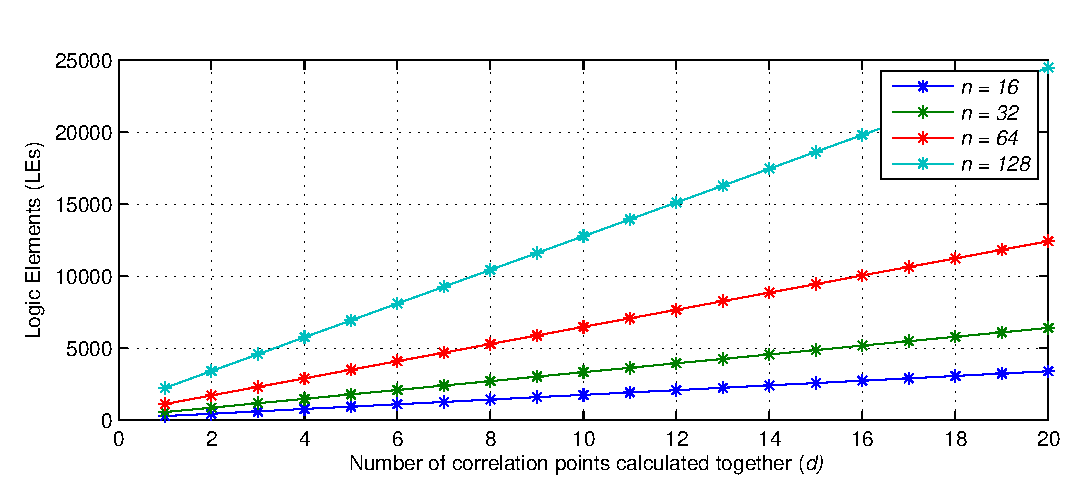
\includegraphics[width=1\linewidth]{./figures/ppt_correlator_perf_16b}
%   \caption{A subfigure}
%   \label{fig:sub1}
% \end{subfigure}%
% \begin{subfigure}{.5\textwidth}
%   \centering
%   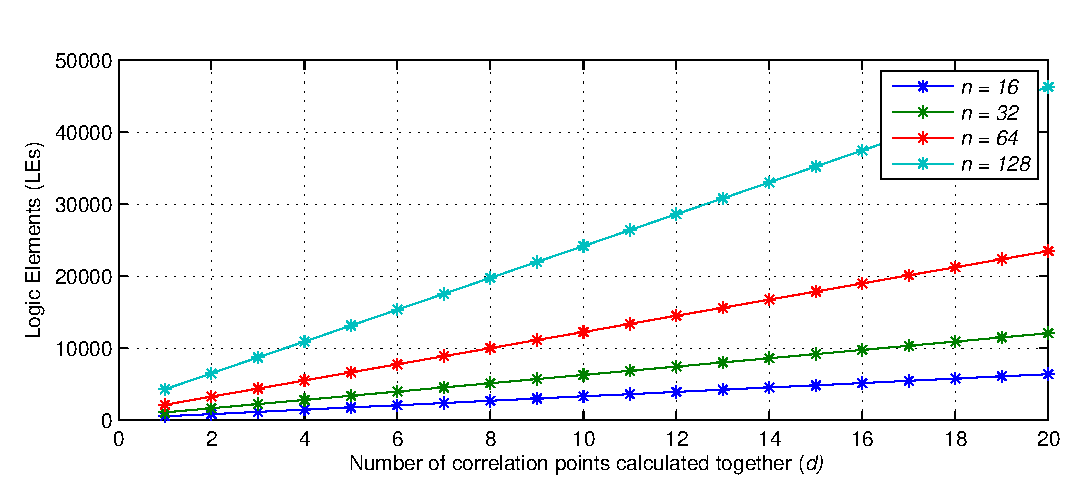
\includegraphics[width=1\linewidth]{./figures/ppt_correlator_perf_32b}
%   \caption{A subfigure}
%   \label{fig:sub2}
% \end{subfigure}
% \caption{A figure with two subfigures}
% \label{fig:test}
% \end{figure}

 \begin{figure}[!hbt]
  \centering
    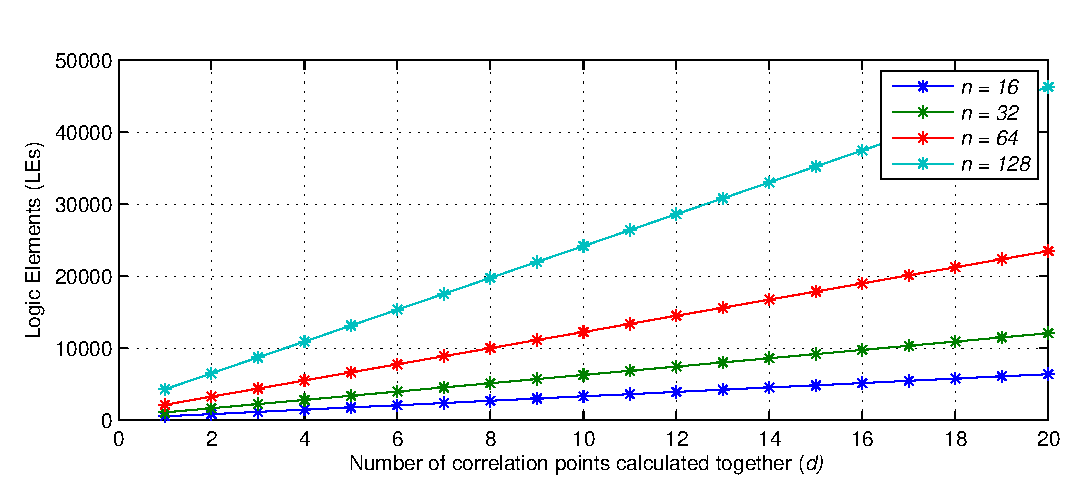
\includegraphics[width=0.9\textwidth]
      {./figures/ppt_correlator_perf_32b}
%     \rule{35em}{0.5pt}
  \caption{Altera's PPT Correlator LEs}
  \label{fig:ppt_correlator_les}
\end{figure}
 
%  \begin{figure}[!hbt]
%   \centering
%     \includegraphics[width=0.8\textwidth]
%       {./figures/ppt_correlator_altera}
% %     \rule{35em}{0.5pt}
%   \caption{Altera's PPT Correlator Architecture}
%   \label{fig:ppt_correlator}
% \end{figure}
 

% \begin{table}[htb]\small
% \centering
% \caption{LEs consumed by the complex multiplier and PPT Correlator}
% \label{table:les_ppt_complex_mult}   
% \begin{tabular}{lllllll}
% \hline
% Entity		         & \thead{Samples processes \\ together ($n$)}	& \thead{Correlation points\\ calculated together ($d$) }  		& 	\thead{ Lenght  \\ (L)}			& \thead{Bitwidth \\ (b)} &  \thead{Logic Elements \\ (LEs)}	\\ \hline
% \textbf{ICFO}              			& \textbf{973.8}			& \textbf{1769}			& \textbf{772}		& \textbf{16128}   	\\ 
% Peak Search			&\hspace{0.3cm}473   	&\hspace{0.3cm}909  		&\hspace{0.3cm}665		& 		-			    \\
% Multiplier/Conjugate      &\hspace{0.3cm}465 		&\hspace{0.3cm}798  		&\hspace{0.3cm}86 		& \hspace{0.3cm}7680  	\\

% FIFO Memories	     	 	&\hspace{0.3cm}35.8 	&\hspace{0.3cm}62			&\hspace{0.3cm}21		& \hspace{0.3cm}8448	\\
% \hline

% \end{tabular}
% \vspace{-0.3cm}
% \end{table}

% The result of equation~\ref{eq:LEs} is of $4574.1$, but since our data is complex, i.e in phase
%  and quadrature component, the result is multiplied by two, therefore the total number of logic 
% elements needed by the correlator is of $9148.2$. Comparing this result with the result 
% obtained by the logic synthesis in FPGA (table~\ref{table:results_fpga_cfo_by_entity}) we see that the total
% number of ALMs, of the complex multiplier (the only block that different in the two designs) is
% of 10. Each ALM is approximately $2.65$ logic elements for a Cyclone V device, thus the total 
% number of logic elements in the complex multiplier is of $26.5$. That is a difference of $9121.5$
% logic elements, so we can conclude that this architecture saves alot of resources.   
 
 \begin{figure}[!hbt]
  \centering
    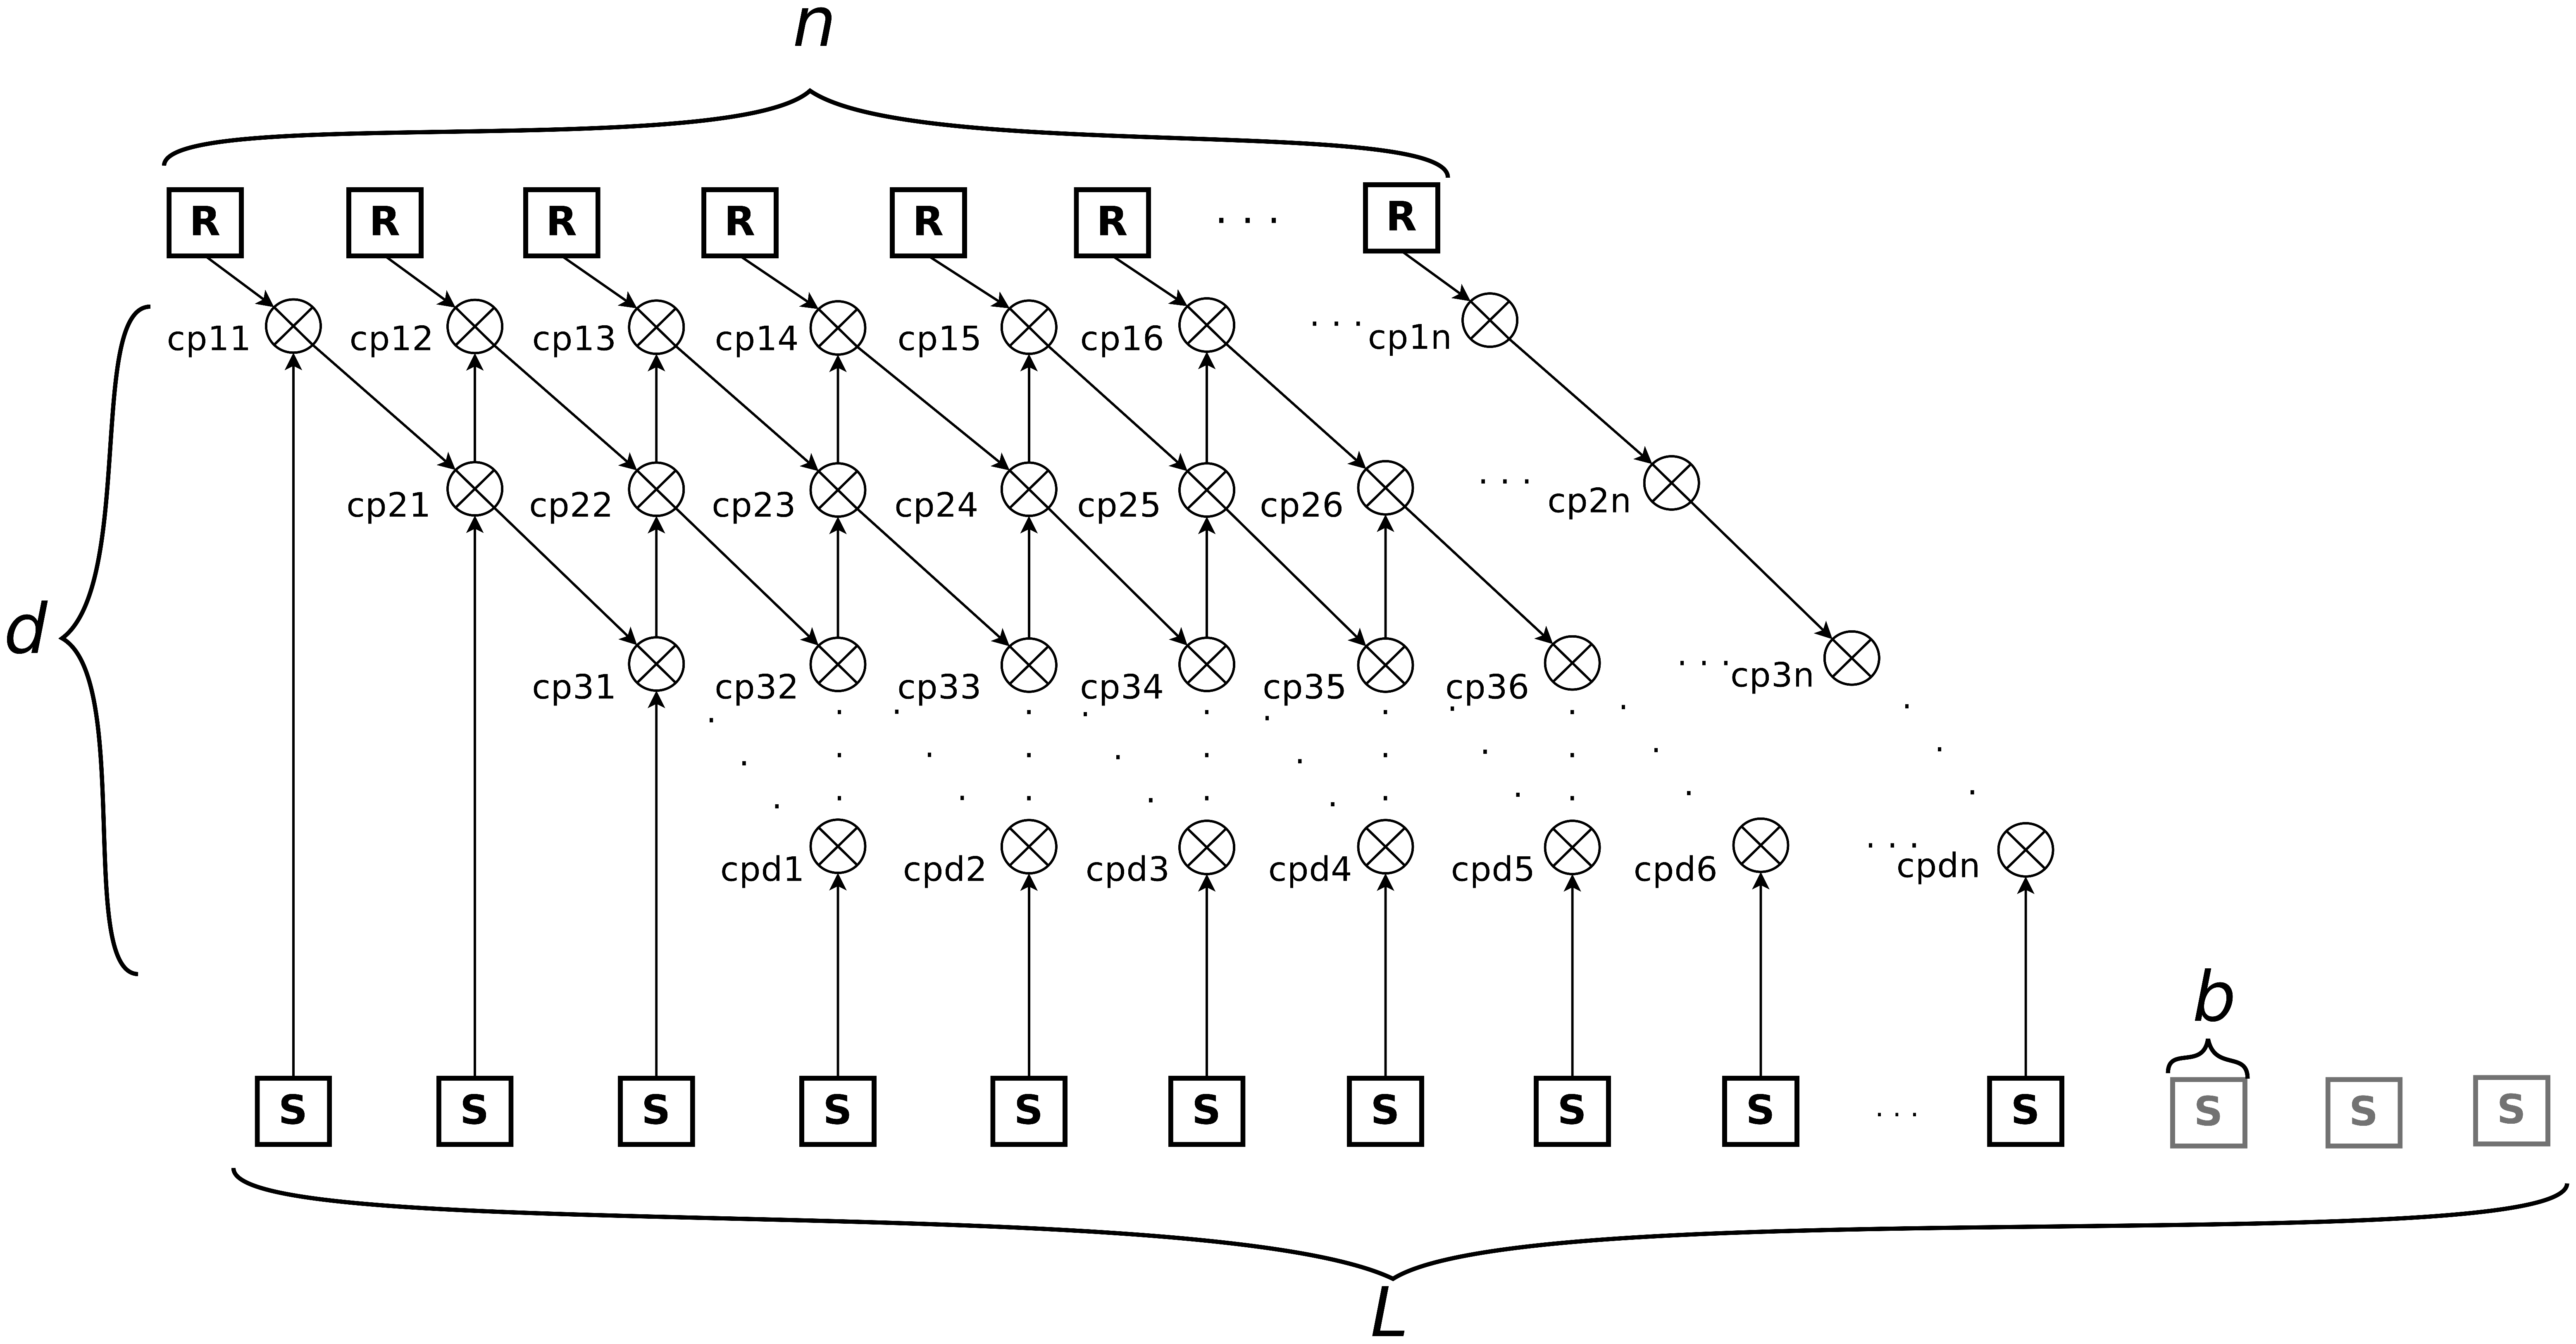
\includegraphics[width=1\textwidth]
      {./figures/ppt_correlator_altera.eps}
%     \rule{35em}{0.5pt}
  \caption{Altera's PPT Correlator Architecture}
  \label{fig:ppt_correlator}
\end{figure}
 
 
 
 
 
\begin{figure}[!hbt]
  \centering
    \includegraphics[width=0.8\textwidth]
      {./figures/int_cfo_arch_2}
%     \rule{35em}{0.5pt}
  \caption{Integer carrier frequency offset estimator/corrector with correlator}
  \label{fig:arq_cfo_2}
\end{figure}



\section{ICFO and STO }

Since the first step in the OFDM synchronization process is the timing synchronization and at this stage channel impairments, noise and CFO is still present in the signal, perfect timing estimation is always difficult to achieve. Algorithms that estimate the timing offset are not robust and residual time offset is often not entirely corrected.  


A more realistic approach to the ICFO estimation is to take into account this residual offset, in figure~\ref{fig:xcorr_sfo_exm} the results of the simulation for the FFT based correlation algorithm for a signal with STO of type II is shown. As can be seen, the correlation result does not yield a maximum value, hence not being able to find the ICFO. This is due to the shifting of the sequence in time, since the data is shifted regarding the LTF reference, the pointwise multiplication performed in time domain does not yield the same result. %Alternatives and analysis of results based on the hardware costs of this and others methods are presented briefly in the next section. 


\begin{figure}[hbt]
  \centering
    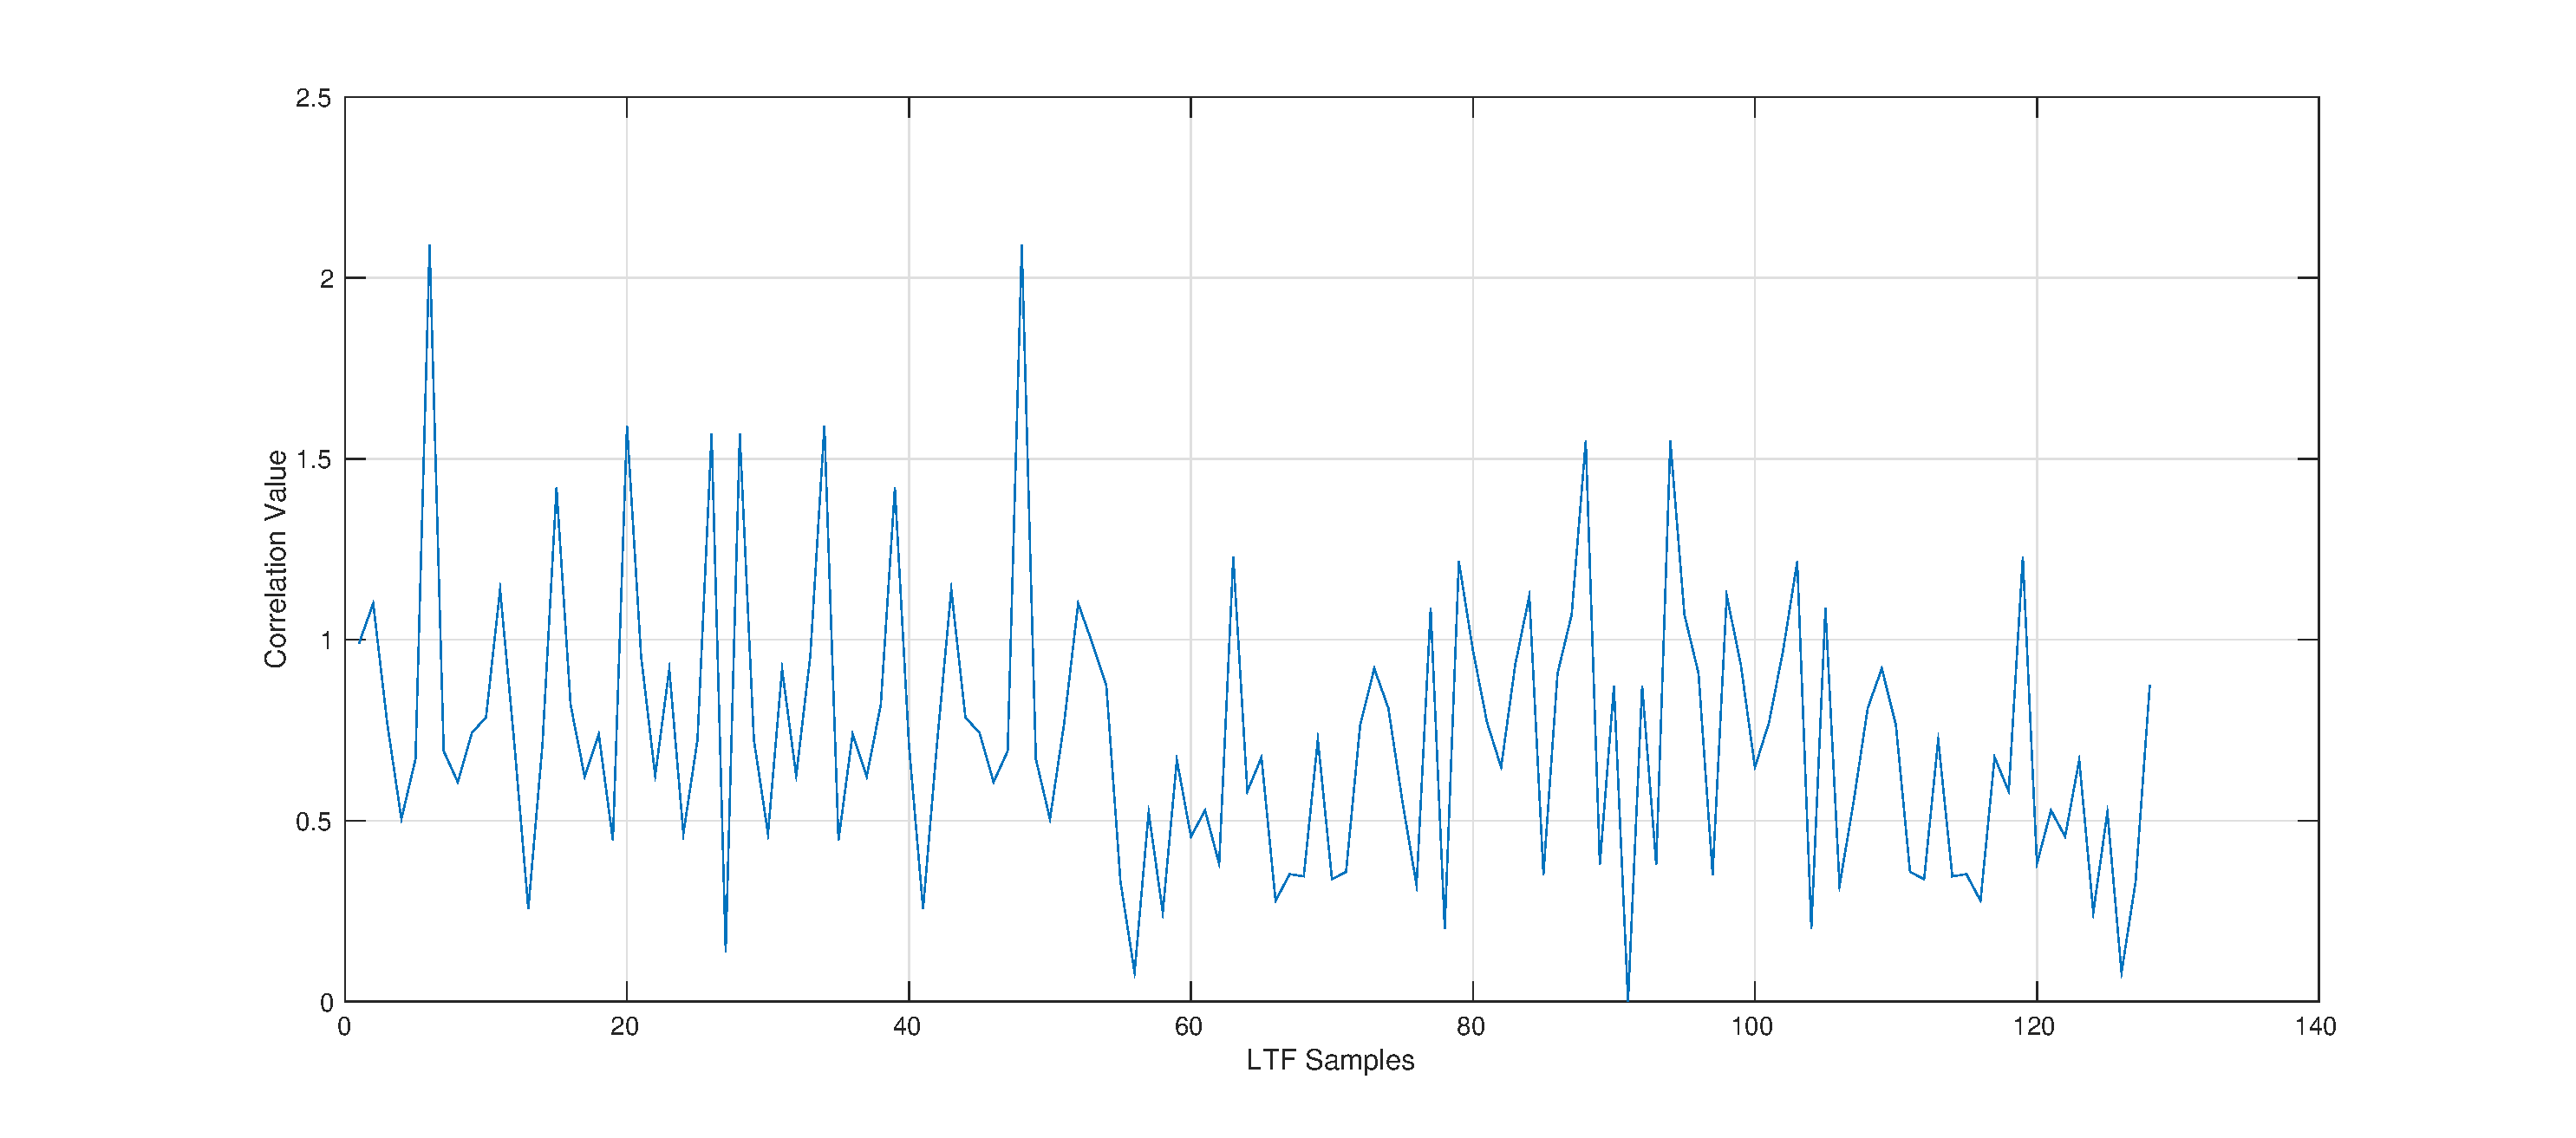
\includegraphics[width=1\textwidth]
      {./figures/correclation_result_sz128_err33_sto}
%     \rule{35em}{0.5pt}
  \caption{LTF Cross-Correlation output with SFO}
  \label{fig:xcorr_sfo_exm}
\end{figure}

\subsubsection{Canet Fine STO estimation}
An algorithm that tries to estimate this residual time offset is presented in~\cite{time_sync_canet}, Canet shows a data aided fine time synchronization method based on the cross-correlation for the IEEE802.11a/g standard, a standard that has a similar PPDU structure than that of the IEEE802.15.4g. Here, fine time synchronization is performed using a cross-correlation between the first 32 samples of the LTF sequence in time domain of the IEEE802.11.ag standard, as in eq~\ref{eq:xcorr_canet_fine_time}. 

 \begin{equation} 
%    y_n=\textbf{\textit{x}}^\intercal_n\cdot \textbf{\textit{w}}_n
C_n = g_{32}^{H}r_n
    \label{eq:xcorr_canet_fine_time}
\end{equation}


\begin{equation}
     r_n=\begin{bmatrix}
         r_{n} & r_{n+1}  & \cdots &  r_{n+31}
        \end{bmatrix}^{T}
\end{equation}

\begin{equation}
     g_{32}=\begin{bmatrix}
         LS_{0} & LS_{1} &  \cdots &  LS_{31}
        \end{bmatrix}^{T}
\end{equation}

Where $r_n$ is the received signal and $g_{32}$ are the first 32 samples of the LTF sequence, the result of the correlation for a fine STO of 10 samples, a signal without ICFO and 20db of noise is shown in figure~\ref{fig:xcorr_sfo_exm_canet}, clearly the correlation output shows a peak value at sample \emph{correlation size - STO}, sample 22 in this case. Results for a noisy channel and type II STO (refer to~\ref{sec:symbol_time_offset}) for a 128 size symbol and CP $1/4$ of symbol size with no ICFO is shown in figure. Two scenarios where tested, in the first the range of the STO is constrained to the CP size (32 samples), that is, the STO varies between 1 samples and 32 samples, on the second the size of the STO is constrained to only 16 samples. It is worth noticing that this algorithms does not works well for STOs greater than half the CP size, as can be seen from the results, a perfect estimation is only achievable when the STO is between 1 and 16 samples. Although good performance under a noisy environment is achieved with this algorithm, it does not work with ICFO as mentioned in~\ref{fig:xcorr_sfo_exm_canet}, so it must be compensated before the fine STO estimation. 




\begin{figure}[hbt]
  \centering
    \includegraphics[width=1\textwidth]
      {./figures/fine_sto_example_80211}
%     \rule{35em}{0.5pt}
  \caption{Example of the computation of fine STO by Canet Method}
  \label{fig:xcorr_sfo_exm_canet}
\end{figure}


\begin{figure}[hbt]
  \centering
    \includegraphics[width=1\textwidth]
      {./figures/fine_sto_canet_32.eps}
%     \rule{35em}{0.5pt}
  \caption{Probability of Success in Canet STO Estimation Algorithm (STO of 32 samples)}
  \label{fig:xcorr_sfo_exm_canet}
\end{figure}


\begin{figure}[hbt]
  \centering
    \includegraphics[width=1\textwidth]
      {./figures/fine_sto_canet_16.eps}
%     \rule{35em}{0.5pt}
  \caption{Probability of Success in Canet STO Estimation Algorithm (STO of 16 samples)}
  \label{fig:xcorr_sfo_exm_canet}
\end{figure}


% \begin{figure}
% \centering
% \begin{subfigure}{.5\textwidth}
%   \centering
%   \includegraphics[width=1\linewidth]{./figures/fine_sto_canet_16}
%   \caption{An STO of 16 samples}
%   \label{fig:sub1}
% \end{subfigure}%
% \begin{subfigure}{.5\textwidth}
%   \centering
%   \includegraphics[width=1\linewidth]{./figures/fine_sto_canet_32}
%   \caption{An STO of 32 samples}
%   \label{fig:sub2}
% \end{subfigure}
% \caption{Probability of success for the Canet STO estimation algorithm}
% \label{fig:test}
% \end{figure}


%results in~\cite{time_sync_canet}, show good performance is achieved with this method, it does not work with CFO. The ambiguous problem is present in the time domain, frequency errors hinders the computation of the STO in time domain, and STO hinders the computation of the CFO in frequency domain. 

%Another approach would be to try to estimate a fine time offset, a more precise time estimation to have certainty that the point chosen is the exactly the symbol start. One approach could be to find the residual time offset in frequency domain aided by the training sequences as proposed in~\cite{doc_thesys_sync}. 

\subsubsection{Non Data Aided STO Estimation}
Repetitive structures in the received signals can be used to decide the symbol start, as is the case of the CP, that repeats itself since a copy of the OFDM symbol is pre-pended to itself to avoid ISI. Algorithms that behave this way are called Non Data Aided or blind synchronization algorithms since no known sequence is used to estimate the symbol start. Although this kind of algorithms are suitable for continuous transmissions and the IEEE802.15.4g standard defines a packet by packet oriented protocol, its analysis determines the difficulty of the estimation of the fine symbol start problem.   


In Non-data aided or blind STO CP based algorithm usually two sliding windows spaced by the symbol length are correlated in time domain. In~\cite{cho2010mimo} an STO estimation technique using the symbol CP is presented, it estimates the STO by taking the difference between the two halves of the size of the CP separated by the symbol size, equation~\ref{eq:diff_cp} shows the operation. In eq.\ref{eq:diff_cp}, $y_{l}$ is the received noisy signal, $N_{cp}$ is the CP size, $N$ the symbol size and $\hat{\sigma}$ is the estimated time offset from a set of $\Sigma$ possible values. Therefore, when the difference between the two halves is minimum the similarity between them is maximum yielding the starting point. This algorithm shows immunity to CFO. Figure \ref{fig:sto_esti_cp_sqrt_diff_example} shows an example of the square difference algorithm for a time offset of 10 samples. Here, symbol size is of 128 samples and CP size 32 samples. 

 \begin{equation} 
%    y_n=\textbf{\textit{x}}^\intercal_n\cdot \textbf{\textit{w}}_n
\hat{\sigma} = \arg\min\limits_{\sigma \epsilon \Sigma} \{ \sum\limits_{n=0}^{N_{cp}-1} (| y_l[n+\sigma] |  - |y_{l}^{*}[n+\sigma+N]|)^2  \}
    \label{eq:diff_cp} 
\end{equation}

\begin{figure}[hbt]
  \centering
    \includegraphics[width=0.9\textwidth]
      {./figures/time_estimation_example_cps_diff}
%     \rule{35em}{0.5pt}
  \caption{Example of the results of the square difference algorithm}
  \label{fig:sto_esti_cp_sqrt_diff_example}
\end{figure}

Another blind algorithm that shows immunity to CFO is presented in \cite{doc_thesys_sync}, it estimates the starting point by using the auto-correlation function. The operation is shown in eq.~\ref{eq:acf_cp}. Here, when the correlation is maximum so is the similarity between the halves. Figure \ref{fig:sto_esti_cp_sqrt_acf_example} show the results of the ACF algorithms for a time offset of 10 samples. A symbol size of 128 and 32 samples of CP are used.   

\begin{equation} 
%    y_n=\textbf{\textit{x}}^\intercal_n\cdot \textbf{\textit{w}}_n
\hat{\sigma} = \arg\max\limits_{\sigma \epsilon \Sigma}  \{ |\sum\limits_{n=0}^{N_{cp}-1} ( y_l[n+\sigma]y_{l}^{*}[n+\sigma+N]) | \} 
    \label{eq:acf_cp} 
\end{equation}

\begin{figure}[hbt]
  \centering
    \includegraphics[width=0.9\textwidth]
      {./figures/time_estimation_example_cps_acf}
%     \rule{35em}{0.5pt}
  \caption{Example of the results of the auto correlation function algorithm}
  \label{fig:sto_esti_cp_sqrt_acf_example}
\end{figure}


Figure~\ref{fig:sto_esti_cp_prob_diff_acf}, shows the probability of success for the CP based methods of equations ~\ref{eq:diff_cp} and~\ref{eq:acf_cp} for a noisy channel in presence of ICFO for all OFDM Options. In this scenario a symbol taken after the SHR was used, that is all the estimations where performed adding noise to the an random generated symbol, then equation ~\ref{eq:diff_cp} and~\ref{eq:acf_cp} where used to estimate the STO. The correlated sequences sizes is of 1/4 symbol size, the size of the CP. It can be seen from figure~\ref{fig:sto_esti_cp_prob_diff_acf} that the method based on the square difference shows better performance than that of the ACF method, in fact the ACF fails at achieving an optimal estimation even for small noise values. As can be seen from fig. \ref{fig:sto_esti_cp_sqrt_diff_example} and fig.~\ref{fig:sto_esti_cp_sqrt_acf_example} a plateau is found at the minimum value of the curve for the square difference algorithm, which means that the differences between estimated values is small between adjacent $\sigma$ values, thus, the minimum value is affected greatly by noise, similar behavior can be seen for the ACF algorithm, adjacent values in magnitude of the autocorrelation show smalls differences, thus being . %Improvement in this method can be accomplished by giving a gain in the samples before performing the difference as shown in eq.\ref{eq:diff_cp_gain}, the values are then multiplied by a $H$ integer value.

% \begin{figure}[hbt]
%   \centering
%     \includegraphics[width=0.9\textwidth]
%       {./figures/prob_sucess_cp_both}
% %     \rule{35em}{0.5pt}
%   \caption{Probability of success of the CP based methods in a noisy channel}
%   \label{fig:sto_esti_cp_prob_diff_acf}
% \end{figure}

\begin{figure}[hbt]
  \centering
    \includegraphics[width=0.9\textwidth]
      {./figures/p_sucess_sto_cps}
%     \rule{35em}{0.5pt}
  \caption{Probability of success of the CP based methods in a noisy channel for all OFDM Options}
  \label{fig:sto_esti_cp_prob_diff_acf}
\end{figure}



% \begin{equation} 
% %    y_n=\textbf{\textit{x}}^\intercal_n\cdot \textbf{\textit{w}}_n
% \hat{\sigma}_{H} = \arg\min\limits_{\sigma \epsilon \Sigma} \{ \sum\limits_{n=0}^{N_{cp}-1} (H|y_l[n+\sigma] |  - H|y_{l}^{*}[n+\sigma+N]|)^2  \}
%     \label{eq:diff_cp_gain} 
% \end{equation}

%gets close to the second half, and after this occurs. So, when noise is added to the system, this minimum difference is affected by it, causing the wrong estimation value. An example of this behavior is shown in figure. On the other hand, the ACF based algorithm shows good results under a noisy environment. 

\subsubsection{Fine STO estimation in frequency domain}
A fine synchronization algorithm presented also in~\cite{cho2010mimo}, estimates the STO in frequency domain using training sequences. According to eq.~\ref{eq:symbol_rx_sto_3}, the time error introduces a phase shift that is constant, thus, if $Y[k]=Y[k-1]$, the phase difference between adjacent carriers must be equal. eq.~\ref{eq:sto_freq} shows the mathematical operation. 

\begin{equation} 
\hat{\sigma} = \frac{N}{2\pi} \arg \{  \sum\limits_{k=1}^{N-1} (Y[k]Y^{*}[k-1]  ) \}
\label{eq:sto_freq} 
\end{equation}

Since the training sequence samples are not completely equal (as required by ~\ref{eq:sto_freq}) in the LTF field  of the synchronization header for the IEEE802.15.4g standard, a slightly modification to eq.~\ref{eq:sto_freq} must be made. Taking the absolute value of every component of the complex samples yields eq.~\ref{eq:sto_freq_154g} 


\begin{equation} 
\hat{\sigma} = \frac{N}{2\pi} \arg \{  \sum\limits_{k=1}^{N-1} |\Re{(Y[k]Y^{*}[k-1])|} + |\Im{(Y[k]Y^{*}[k-1])|} \} 
\label{eq:sto_freq_154g} 
\end{equation}

The probability of correct STO estimation for the data aided phase difference in frequency domain for all OFDM Options is shown in figure~\ref{fig:sto_esti_freq_rstl}. For this algorithm the probability of success decreases with the symbol size, for smaller symbols the probability improves. The probability of success of the three STO estimation methods for a noisy channel is shown in \ref{fig:sto_esti_all_rstl} for all OFDM Options. The data aided algorithm (the phase difference in frequency domain) shows better results than the Non data Aided CP based ones, it achieves a perfect residual timing estimation for a SNR greater than 10db for the OFDM Option 4 and SNR greater than 20db for Option 1, while only the square difference algorithm achieves close to optimal optimization after only 40db.

%%%%%ONLY OPT1
% \begin{figure}[hbt]
%   \centering
%     %\includegraphics[width=1\textwidth]
%     \includegraphics[width=0.9\textwidth]
%       {./figures/p_sucess_sto_freq}
% %     \rule{35em}{0.5pt}
%   \caption{Probability of success in estimating the STO for the data aided frequency domain algorithm}
%   \label{fig:sto_esti_freq_rstl}
% \end{figure}

\begin{figure}[hbt]
  \centering
    %\includegraphics[width=1\textwidth]
    \includegraphics[width=1\textwidth]
      {./figures/p_sucess_sto_freq_ch0}
%     \rule{35em}{0.5pt}
  \caption{Probability of success in estimating the STO for the data aided frequency domain algorithm for all OFDM Options}
  \label{fig:sto_esti_freq_rstl}
\end{figure}

%%%%%ONLY OPT1
% \begin{figure}[hbt]
%   \centering
%     %\includegraphics[width=1\textwidth]
%     \includegraphics[width=0.9\textwidth]
%       {./figures/prob_sucess_cp_all}
% %     \rule{35em}{0.5pt}
%   \caption{Probability of success in estimating the STO}
%   \label{fig:sto_esti_all_rstl}
% \end{figure}


\begin{figure}[hbt]
  \centering
    %\includegraphics[width=1\textwidth]
    \includegraphics[width=1\textwidth]
      {./figures/p_sucess_sto}
%     \rule{35em}{0.5pt}
  \caption{Probability of success in estimating the STO for all OFDM Options}
  \label{fig:sto_esti_all_rstl}
\end{figure}


% \begin{figure}[hbt]
%   \centering
%     %\includegraphics[width=1\textwidth]
%     \includegraphics[width=0.8\textwidth]
%       {./figures/prob_sucess_sto_all_channel}
% %     \rule{35em}{0.5pt}
%   \caption{Probability of success in estimating the STO}
%   \label{fig:sto_methods_all}
% \end{figure}

Another factor that hinders the proper demodulation of the incoming signals that has not been taken into account is the signal degradation caused by the frequency selective channel. Simulation results for a frequency selective channel are shown in figure~\ref{fig:sto_esti_cp_diff_chn} and figure~\ref{fig:sto_esti_cp_acf_chn} for the square difference and the ACF based algorithm respectively. Both CP based algorithms show degradation in performance for a noisy and frequency selective channel, since both algorithms depend on the CP to estimate the STO.

Results for the phase difference in the frequency domain are shown in figure \ref{fig:sto_esti_ph_diff_chn}, this algorithm fails at estimating the residual STO. Not only a degradation in the estimation is shown as in the CP based algorithms, but a completely inexact estimation is shown. The probability of deviation in samples from the ideal estimated value for the frequency selective channel is shown in figure~\ref{fig:sto_esti_dev_ph_diff_chn} for a SNR of 20db. Figure~\ref{fig:sto_esti_dev_ph_diff_chn} shows that the frequency selective channel model used for this simulation introduces a phase shift in the frequency domain that is constant and that causes a different estimated value of the residual STO. 

%The estimation value given by the phase difference in frequency algorithm is then that of the phase difference caused by the STO plus a phase difference caused by the frequency selective channel. At this point it is not possible to determine the phase change introduced by the channel, thus it is not possible to estimate accurately the STO by means of the phase difference algorithm in presence of a frequency selective channel. 

% Another factor that hinders the proper demodulation of the incoming signals that has not been taken into account is the inter symbol interference caused by the frequency selective channel. Simulation results for a frequency selective channel are shown in figure~\ref{fig:sto_esti_cp_diff_chn} and figure~\ref{fig:sto_esti_cp_acf_chn} for the square difference and the ACF based algorithm respectively. Both CP based algorithms show degradation in performance for a noisy and frequency selective channel, since both algorithms depend on the CP to estimate the STO, and this is corrupted by the frequency response of the channel. Results for the phase difference in frequency domain are shown in figure x, this algorithm fails at estimating the residual STO. Not only a degradation in the estimation is shown as in the CP based algorithms, but a completely inexact estimation is shown. The probability of deviation in samples from the ideal estimated value for the current used channel is shown in figure x for a SNR of 2db. Figure shows that the frequency selective channel introduces a phase shift in frequency domain that is constant and that causes a wrong estimated value of the residual STO. At this point it is not possible to know how much the channel introduces in the phase difference estimated, therefore no compensation can be performed for this method. 


% Performance of the ICFO estimation algorithm combined with the STO estimation algorithms is shown in figure~\ref{fig:icfo_sucess_sto_correction}. The frame start is corrected according to the estimated value given by the CP and phase difference in frequency algorithms, and then the ICFO is estimated according to equation~\ref{eq:xcorr_theorem_tf}. 

\begin{figure}[hbt]
  \centering
    \includegraphics[width=0.9\textwidth]
      {./figures/p_sucess_sto_diff_cps}
%     \rule{35em}{0.5pt}
  \caption{Probability of success in estimating the STO for CP based square difference under a frequency selective Channel}
  \label{fig:sto_esti_cp_diff_chn}
\end{figure}


\begin{figure}[hbt]
  \centering
    \includegraphics[width=0.9\textwidth]
      {./figures/p_sucess_sto_acf_chn_all}
%     \rule{35em}{0.5pt}
  \caption{Probability of success in estimating the STO for CP based ACF under a frequency selective Channel}
  \label{fig:sto_esti_cp_acf_chn}
\end{figure}


%%%Only Option 1
% \begin{figure}[hbt]
%   \centering
%     \includegraphics[width=0.9\textwidth]
%       {./figures/prob_sucess_sto_ph_diff_ch}
% %     \rule{35em}{0.5pt}
%   \caption{Probability of success in estimating the STO for the phase difference in frequency domain algorithm under a frequency selective channel}
%   \label{fig:sto_esti_ph_diff_chn}
% \end{figure}

\begin{figure}[hbt]
  \centering
    \includegraphics[width=0.9\textwidth]
      {./figures/p_sucess_sto_freq_all}
%     \rule{35em}{0.5pt}
  \caption{Probability of success in estimating the STO for the phase difference in frequency domain algorithm under a frequency selective channel for all OFDM Options}
  \label{fig:sto_esti_ph_diff_chn}
\end{figure}


\begin{figure}[hbt]
  \centering
    \includegraphics[width=0.9\textwidth]
      {./figures/prob_deviation_ph_freq}
%     \rule{35em}{0.5pt}
  \caption{Probability of deviation for the phase difference in frequency domain algorithm}
  \label{fig:sto_esti_dev_ph_diff_chn}
\end{figure}

% \begin{figure}[hbt]
%   \centering
%     \includegraphics[width=0.9\textwidth]
%       {./figures/prob_sucess_icfo_w_sto_correction}
% %     \rule{35em}{0.5pt}
%   \caption{Probability of success in estimating the ICFO after computing the STO with the proposed algorithms}
%   \label{fig:icfo_sucess_sto_correction}
% \end{figure}

Results from the residual STO estimation show very poor performance for a noisy and frequency selective channel, neither the CP based approaches nor the phase difference in frequency domain approach achieves a perfect STO estimation even for low level noise, the square difference  algorithm shows the best performance of the three algorithms. The poor performance of the phase difference in frequency domain also shows that even though the estimation using this method shows a phase shift introduced by the channel in frequency domain, it not implies a displacement in the OFDM symbol samples in time domain, as it happens with the residual time offset. It is not possible to know at this point in the process the actual contribution of the channel to the phase shift estimated, hence it is impossible to compensate the error introduced by it.  


%------------------------------ICFO-----------------------------------------------------------
\subsubsection{ICFO Estimation in frequency domain with immunity to STO}

Another approach is to try to estimate the ICFO even with the residual timing error, which is the case of the work presented by BoAi in~\cite{boai_icfo}, here a data aided algorithm in frequency domain which is not affected by timing errors is presented. The operation is as described in  eq.~\ref{eq:boai_m3} 

\begin{equation} 
\hat{M} = \max\limits_{l \epsilon L}\{{\sum\limits_{k=1}^{W} | Y_{m, k}X^{*}_{m, k + l}} | \}
\label{eq:boai_m3}
\end{equation}

Here, $W$ is the number of continuous samples, $Y_{m, k}$ is the $k^{th}$ sample of the $m^{th}$ received noise corrupted OFDM symbol after the FFT, $X_{m, k}$ is the uncorrupted reference in frequency domain, $L$ is the estimation range, and $l$ the sliding window. 

\begin{figure}[hbt]
  \centering
    \includegraphics[width=0.9\textwidth]
      {./figures/correclation_result_sz128_err35_sto_boai}
%     \rule{35em}{0.5pt}
  \caption{Example in estimating a ICFO of 35 carriers for the BoAi Proposed Method}
  \label{fig:xcorr_boai_exm}
\end{figure}

Figure~\ref{fig:xcorr_boai_exm} shows the result of the BoAi algorithm for a residual STO no greater than the CP size, additive white gaussian noise and a ICFO of 35 subcarriers for a symbol size of 128 samples. The result of the correlations shows that a maximum peak value is found at the sample 35, the actual ICFO in the signal. 

%Performance of this algorithm is shown in figure \ref{fig:boai_probability_success}.

%As is shown in the result the estimation of the ICFO in the frequency domain taking the maximum of the correlation values is unaffected by the residual timing offset. This algorithm show good results even with STO.


\subsubsection{FFT Based ICFO Estimation with immunity to STO}
Although computing the cross correlation by means of eq.~\ref{eq:xcorr_theorem_tf} between the training sequences in presence of a small STO does not yields the actual ICFO, the correlation must yield a maximum value when the similarity between two signals is maximum. In this sense, the ICFO must yield a maximum value from within a set of maximum of correlations values. Finding the correlations of the shifted signals with STO, must yield a maximum when those signals similarities are maximized, that is when the STO is equal to zero. eq.~\ref{eq:xcorr_max} shows the mathematical operation. Here, $y(n)$ is the received long training sequence in the time domain, $x(n)$ is the reference training sequence also in time domain and $\odot$ implies pointwise multiplication between $y$ and $x$. An example of the maximum of correlations is shown in figure \ref{fig:xcorrmax_example}, here a 128 samples symbols is used, an STO of 7 samples and a ICFO of 23 subcarriers. Clearly, a peak value if found for the eighth correlation (when the STO becomes 0) in the 23rd sample of that correlation. 
%This method manages to give  



\begin{equation} 
\hat{\theta} = \max\limits_{\theta} [ \max { \mathcal{F}[y(n+\theta) \odot x^{*}(n)] }  ]
\label{eq:xcorr_max}
\end{equation}

\begin{figure}[hbt]
  \centering
    \includegraphics[width=1\textwidth]
      {./figures/max_corre_example}
%     \rule{35em}{0.5pt}
  \caption{Example of the maximum of correlations method for estimating the ICFO }
  \label{fig:xcorrmax_example}
\end{figure}


Performance of the BoAi algorithm and the maximum of correlations method for all OFDM options in presence of only white noise is presented in figure \ref{fig:boai_xcorrmax_results}. As can be seen the maximum of correlations outperforms the Boai algorithm by approximately 15 db, it reaches a perfect ICFO estimation at approximately -20db, while the BoAi algorithm at approximately -5db. Figure \ref{fig:boai_xcorrmax_results_channel_freq} shows the performance results of both algorithms without a frequency selective channel (WoC) and with a frequency selective channel (WC), here the results is almost the same as with only white noise, the frequency selective channel does not affect much the estimation for both algorithms. It is worth noticing that for the option with the least number of carriers, OFDM Option 4, the BoAi algorithms fails to estimate correctly the ICFO, this is not the case for the ICFO.  


\begin{figure}[hbt]
  \centering
    \includegraphics[width=0.9\textwidth]
      {./figures/p_sucess_icfo_all_alg_ch0}
%     \rule{35em}{0.5pt}
  \caption{Probability of success in estimating the ICFO for the BoAi and maximum of correlations Proposed Methods for all OFDM Options}
  \label{fig:boai_xcorrmax_results}
\end{figure}



\begin{figure}[hbt]
  \centering
    \includegraphics[width=0.9\textwidth]
      {./figures/p_sucess_icfo_ch_all}
%     \rule{35em}{0.5pt}
  \caption{Probability of success in estimating the ICFO for the BoAi and maximum of correlations Proposed Methods for all OFDM Options under a frequency selective channel}
  \label{fig:boai_xcorrmax_results_channel_freq}
\end{figure}

%ONLY OPTION 1
% \begin{figure}[hbt]
%   \centering
%     \includegraphics[width=0.9\textwidth]
%       {./figures/p_sucess_boai_xcorrmax_algorithms}
% %     \rule{35em}{0.5pt}
%   \caption{Probability of success in estimating the ICFO for the BoAi and maximum of correlations Proposed Methods}
%   \label{fig:boai_xcorrmax_results}
% \end{figure}



From the results obtained for the STo and ICFO estimation we can conclude that the blind techniques tested show much worse performance than that of the data aided techniques for a noisy channel, also the a robust estimation of the STO is difficult to achieve at this point in the synchronization process, channel impairments as well as frequency errors are still present in the signal making it difficult to estimate a perfect symbol time offset even for high SNR values. A small residual time offset that falls in the CP of the symbol can be corrected by the one tap equalizer~\cite{sto_equalization}, so perfect estimation is not completely needed in the OFDM synchronization process. 

% \begin{figure}[hbt]
%   \centering
%     \includegraphics[width=0.9\textwidth]
%       {./figures/prob_sucess_all_algorithms}
% %     \rule{35em}{0.5pt}
%   \caption{Probability of success in estimating the ICFO}
%   \label{fig:icfo_results_all}
% \end{figure}


% Simulations performed in the presence of additive white gaussian noise with the following parameters, FFT size $128$, sampling frequency of $fs = 1.33 Mhz$, length of CP of $16$ samples and subcarrier space $10.4 Khz$ gives the results of figure. 

% Figures show the impact of the different algorithms in the overall OFDM system performance. Here, for a SNR of x, the BER is x for the maximum of correlation algorithms, an improvement of N DBs when compared with BoAi method, and of x dbs when compared with the fine STO estimations method. Good performance is achieved with the proposed method, in the next section the hardware implementation costs of the presented methods is analyzed. 

%\section{ICFO algorithms implementation}

\section{STO and ICFO hardware implementations}

In this sections the cost of implementation of the previously presented methods for estimating the ICFO is presented. Area and throughput are the main parameters to consider for the hardware architectures presented.


\subsection{CP Based Architectures}
As it was shown in section \ref{sec:fft_cfo_architecture}, the CP of the OFDM symbol can be used to perform a not so robust fine time estimation. Two methods where presented employing similar operations to estimate the STO, one is based on the ACF while the other takes the difference between samples. The implementation of those methods are similar in logic as we will see in the following. 


Figure \ref{fig:arq_sto_acf_serial} shows the architecture for the ACF CP Based algorithm. The computation is as follows, for every clock cycle two samples from two windows separated by the symbol size are multiplied, the multiplication result of the window sample and the conjugate sample of the CP size dislocated window, is sent to an adder that sums the current multiplication results with the previous one the result is saved in a register. CP clock cycles after, the current stored value is sent to the CORDIC in circular coordinates in vectoring mode, its output is then the module of the sum, also CP clocks cycles after the first multiplication a total sum counter (Count sums in figure \ref{fig:arq_sto_acf_serial}) is incremented. The computed module is then compared with the previous greater module found, if the current value is greater its valued is saved in \emph{reg ACF} and the current count of the count sums counter counter is saved, the process is repeated shifting the input sequence until the estimated range is reached, in that moment the current stored value of the sums counter is the estimated STO. 

The architecture in figure \ref{fig:arq_sto_acf_serial} is a serial architecture, it computes one operation per clock cycle, the total delay for the maximum CP size for the OFDM option 1 and a estimation range of 10 (a maximum STO of 10 samples) is of 320 clock cycles. 

Figure \ref{fig:arq_sto_diff_serial} shows the architecture for the square difference algorithm, the functioning of this architecture is the same as the ACF, an accumulator followed by a comparator, just that in this case the module of the samples is taken at the input. Two CORDIC blocks (one for each sample, with one of them conjugated) compute the modules input, that are then subtracted and the result finally multiplied by itself, this results then goes to the same structure as in the ACF architecture to compute the STO. The time spent in the computation is the same as in the ACF architecture, CP times the estimation range, for OFDM option 1, 320 clock cycles. 

The delay in the computation time of both architectures can be reduced by parallelizing the multiplication for the ACF and subtraction for the square difference algorithm, and example is shown in figure \ref{fig:arq_sto_cp_parallel} for the ACF architecture, here, the registers are replaced by a series of $n$ registers connected that feed $n/2$ multipliers (4 in the example) and these in turn feed a tree of $n/2-1$ adders. The delay is reduced in $CP/(n/2)$. For the square difference algorithm the multipliers are replaced by subtractors and multipliers, one pair for each complex multiplier. %Table \ref{tab:requir_logic_cp} summarizes the requirements of each architecture. The numbers in parentheses are for the parallel implementation, complex components (as in registers and adders) are counted as double, that is, for the ACF implementation the number of registers at the input (the registers storing the data) must store complex data, i. e. imaginary and real part.  


% \begin{table}[]\footnotesize
% \centering
% %\begin{adjustbox}{max width=\textwidth}
% \caption{Hardware requirements for the CP based hardware implementations}
% \label{my-label}
% \begin{tabular}{ccccccccc} 
% \hline
%                                                             & Registers & \begin{tabular}[c]{@{}c@{}}Multipliers \\ (Complex)\end{tabular} & Mutipliers & Adders & Substractor & Comparators & Counters & CORDIC \\ \hline
% ACF                                                          & 8(20)     & 1(4)                                                             & -          & 2(8)   & -           & 3           & 2        & 1      \\
% \begin{tabular}[c]{@{}c@{}}Square \\ difference\end{tabular} & 5(11)     & -                                                                & 1(4)       & 1(4)   & 1(4)        & 3           & 2        & 2     \\ \hline
% \end{tabular}
%  \label{table:requir_logic_cp}
% %\end{adjustbox}
% \end{table}


 % Two version can be considered for the implementation, a semi-parallel (since a fully parallel version would consume a great amount of resources) and serial version. Figure \ref{fig:arq_sto_cp_parallel} and figure \ref{fig:arq_sto_cp_serial} show both architectures respectively. 

\begin{figure}[!hbt]
  \centering
    \includegraphics[width=0.7\textwidth]
      {./figures/sto_arq_acf_serial}
%     \rule{35em}{0.5pt}
  \caption{Serial Architecture for the CP Based ACF algorithm}
  \label{fig:arq_sto_acf_serial}
\end{figure}


\begin{figure}[!hbt]
  \centering
    \includegraphics[width=0.7\textwidth]
      {./figures/sto_arq_diff_serial}
%     \rule{35em}{0.5pt}
  \caption{Serial Architecture for the CP Square Difference algorithm }
  \label{fig:arq_sto_diff_serial}
\end{figure}

\begin{figure}[!hbt]
  \centering
    \includegraphics[width=0.7\textwidth]
      {./figures/semi_parallel}
%     \rule{35em}{0.5pt}
  \caption{Parallel multipliers in STO ACF architecture}
  \label{fig:arq_sto_cp_parallel}
\end{figure}

% The computation is as follows, from figure \ref{fig:arq_sto_cp_serial}, a multiplication of two samples is performed, then the multiplication result enters an adder tree that outputs the partial sum result. The partial sum is stored in the register \emph{reg_sum}, then the data is shifted in the samples registers and the result of \emph{Adder3} is updated with the sum of the following four values, and \emph{reg_sum} stores the sum of the current 4 values with the previous 4 values. After $CP/4$ clocks an output of the ACF is computed, this output is then sent to the comparator that check if the current computed value is greater than the previous one, if it is, the register \emph{reg_ACF} is updated and the register \emph{reg_idx} stores the index value of the current output calculated. The process stops when the range specified is reached by the counter $\sigma$.

% The serial version logic is the same, the results of the multiplication is stored in a sum register, just that in this case, instead of $CP/4$ clocks cycles, CP clocks are needed by ACF output, only one multiplier and one adder is used.


%This block makes use of the null tones inserted before and after the 
%significant data, known as active tones, appending the correct number of null tones before and after them.

\subsection{Fine STO estimation in frequency domain Architecture} 

Figure \ref{fig:arq_fine_sto_freq} shows the architecture of the fine STO estimator in frequency domain according to equation \ref{eq:sto_freq} using the LTF known sequence, its functioning is as follows, first each carrier of the OFDM symbol in the LTF is multiplied by its conjugate adjacent subcarrier, taking the difference in angle, then the absolute value of each component of the complex signal is computed and the results accumulated for $symbol_size$ cycles (the symbol size). Finally the angle of the sum is computed by means of the CORDIC and the result multiplied by $N/(2*pi)$, this output is then the STO. The delay of this architecture is of one OFDM symbol, e.g. 128 clock cycles are needed to compute the STO for option 4. 

\begin{figure}[!hbt]
  \centering
    \includegraphics[width=0.9\textwidth]
      {./figures/fine_sto_freq}
%     \rule{35em}{0.5pt}
  \caption{Architecture for the Fine STO estimator in frequency domain}
  \label{fig:arq_fine_sto_freq}
\end{figure}

% \begin{table}[]\footnotesize
% \centering
% %\begin{adjustbox}{max width=\textwidth}
% \caption{Hardware requirements for the STO estimator in frequency domain}
% \label{my-label}
% \begin{tabular}{ccccccccc} 
% \hline
% %                                                             & Registers & \begin{tabular}[c]{@{}c@{}}Multipliers \\ (Complex)\end{tabular} & Mutipliers & Adders & Substractor & Comparators & Counters & CORDIC \\ \hline
% ACF                                                          & 8(20)     & 1(4)                                                             & -          & 2(8)   & -           & 3           & 2        & 1      \\
% \end{tabular}
%  \label{table:requir_logic_cp}
% %\end{adjustbox}
% \end{table}

It is worth noticing that this architecture shows poor performance under a frequency selective channel, therefore additional hardware is needed to estimate the channel and compensate its contribution to the signal phase in frequency domain in order to estimate accurately the STO. 

%As can be seen, the implementation of the square difference consumes less resources than the ACF based STO algorithm. Although it performance is lower it has some advantage over the ACF implementation, if hardware consumption is a must the square difference implementation is an option.  


\subsection{BoAi Algorithm Architecture}

 Figure \ref{fig:arq_boai} shows the BoAi implementation for the ICFO. It has some similarities with the CP based implementations, an accumulator and a register saves the current count and sends data to be compared to previous accumulated values. The computation ends when the estimation range is reached, in that moment the ICFO value is the value stores in the index registers, a registry that is updated every time a maximum value is found. 

%current value of the registers of index that is registered when an accumulator value computed is greater than the previous grater value found. 

Since the correlation of this algorithm is performed in frequency domain where the LTF is composed of +/-$1s$ and $0s$, a simpler implementation can be accomplished, the simplification comes in the multiplier at the input of the architecture, since the multiplication is performed in the frequency domain it becomes a 0 or $+1/-1$ multiplication, in hardware that can be accomplished by a series of XOR gates, one for every bit of the sample, followed by an adder. 

%The memory to store the LTF in frequency domain is also much less than that of the LTF in time domain.  

The delay of this architecture if of $128*range$ clock cycles, for example for a estimation range of $10$ subcarriers, 1280 clock cycles are required. As with the CP based architectures the process can be parallelized, XOR multipliers and CORDICs blocks in parallel (one for each sample) allows the reduction of the delay at the cost of more hardware. A parallelization of 4 samples is shown in figure \ref{fig:arq_boai_parallel}, the outputs of the CORDICs blocks are added and sent to the accumulator, the rest of the process remains the same, as with the serial case. The downside of this parallelization is the use of the CORDIC block, which uses lots of resources. The number of clock cycles is reduced to $(Symbol Size)/(parallel instances)*range$, for the example shown in figure \ref{fig:arq_boai_parallel} for a estimation range of 10 carriers,  $128/4*10 = 320$ clock cycles.  

Even though this implementation may use more sources than the STO implementations no additional hardware is required to perform the ICFO estimation, as with the STO architectures, since those architectures requires the the additional hardware of the ICFO shown in figure~\ref{fig:arq_cfo}.

%BoAi presents a simpler hardware implementation since the correlation operation is performed in frequency domain where the LTF is composed of only ones and zeros, hence simpler computations can be performed. 

\begin{figure}[!hbt]
  \centering
    \includegraphics[width=0.7\textwidth]
      {./figures/boai_serial}
%     \rule{35em}{0.5pt}
  \caption{BoAi algorithm implementation}
  \label{fig:arq_boai}
\end{figure}


\begin{figure}[!hbt]
  \centering
    \includegraphics[width=0.7\textwidth]
      {./figures/boai_parallel}
%     \rule{35em}{0.5pt}
  \caption{BoAi algorithm implementation in parallel}
  \label{fig:arq_boai_parallel}
\end{figure}




\subsection{Maximum of correlations Algorithm}

Only a slightly modification to the implementation presented in~\ref{sec:icfo_architecture} is performed for this architecture. At the input a buffer of size $symbol size + STO range$ stores the symbol plus a small group of samples corresponding to the STO ranges to estimate, for every correlation computed the buffer shifts one sample off the buffered sequence. The symbol size sequence is then point-wise multiplied in time domain by the uncorrupted reference LTF and the result sent to the FFT block, the FFT out now goes to the peak searcher that finds a local maximum, then the buffered sequence is shifted and another correlation is computed. This local maximum is then compared with all the local maximums of all the correlations computed, the index of the maximum of local maximums (the global maximum) is the ICFO. The previously peak searcher shown~\ref{sec:icfo_architecture} must then be  changed to compute maximum of maximum values. The new peak searcher block is shown in figure \ref{fig:max_corre_peaks}.  

\begin{figure}[!hbt]
  \centering
    \includegraphics[width=0.9\textwidth]
      {./figures/peak_searcher_new}
%     \rule{35em}{0.5pt}
  \caption{Peak searcher for the FFT based maximum of correlations algorithm}
  \label{fig:max_corre_peaks}
\end{figure}

To find the global maximum (the maximum of the maximum of all the computed correlations) the peak searcher compares the current FFT output with the previous one, every time a maximum value is found its value is stored in the register \emph{reg local max}, in parallel the local index of where this maximum value was found is stored in the register \emph{reg idx max local}. When the samples count reaches the symbol size, the value of the maximum register along with the value of its index is passed to a global comparator that compares the current maximum local value with the previous partial global found, the index value is stores in a auxiliary register, if the current value is greater than the previous one the current value is stored and the global index register is updated with the auxiliary register value. The process ends when the STO range value is reached. 

Since the computation of the ICFO by means of this method involves the FFT computation, the delay of the computation includes the delay of the FFT, which slows down the process. For this method the delay is given by eq \ref{eq:delay_max_xcorr}.

\begin{equation} 
delay_{maxcorr} = (delay_{FFT} + Symbol_{sz})*STO_{range} 
\label{eq:delay_max_xcorr}
\end{equation}

\begin{equation} 
delay_{fft} = \frac{FFT_{sz}}{2}\log_2{FFT_{sz}}  
\label{eq:delay_max_xcorr}
\end{equation}


For a STO of 10 samples and OFMD option 1, the delay of this architecture is of $5760$ clock cycles. The delay of this architecture is the greatest of all the implementations presented. However, some modifications can be done to reduce this delay:

\begin{itemize}
\item \emph{Pipeling the FFT} : with this method the delay of the computation is reduced to $Symbol_{sz}*STO_{range}$. Although it may seem that the advantages of the FFT implementation presented previously are lost with the use of a pipeline architecture, the use of a CORDIC based butterfly that eliminates the use of ROM memories to store twiddle factors can still be used in a pipeline structure. The only disadvantage of the pipeline approach would be hardware reuse, for FFT sizes smaller than 128 much of the hardware occupied by the FFT would remain without utilization. It is worth noticing, that blocks with very large delays halt the system, requiring buffers to compensate those delays. Those buffers hardware requirements that the serial implementation introduces could be more than the size needed by the pipeline version of the FFT, thus requiring an FFT pipelined in the final design, even if there is no FFT based ICFO. A pipelined FFT would allow to implement the presented method without much delay and with advantages over other ICFO implementations, for example the ICFO range that this implementation allows is of a symbol size ($128$ for OFDM option 1), whereas the BoAi implementation requires $128*128$ to estimate the same range of ICFO. The analysis of the requirements and the benefit of the pipeline architecture in the whole MR-OFDM system is still an ongoing task.

\item \emph{Modules running at different clock frequencies} By running different modules at different clocks frequencies, a reduction in blocks delays can be achieved. If the FFT block runs at a higher frequency than that of the rest of the design, the delay of this block can be compensated, this of course has implications in power consumption. 

%the FFT delay and consequently a reduction in the ICFO delay
\end{itemize}
 
 

 %Further results and other variables in the whole design determine this tradeoff, as in the area available for the final chip and power consumption

%is a must, since the intended application is low power, and an architecture that occupies much more hardware could lead to greater power consumption. It is worth remembering that implementations of this kind are not trivial and can take months of development process, but also, the FFT is an important block in the OFDM system, time of development could lead to a much improved design.    

% \item \emph{Reduce the FFT size} : Reducing the range of the ICFO by reducing the size of the FFT computed to perform the correlation the delay can be also reduced, for example, for a 128 size FFT, only the first 32 points of the correlation are computed. This would reduce the computation time at the cost of a reduced ICFO range. 

Tables \ref{table:resources_entity_all_sto} and \ref{table:resources_entity_icfos} show a summary of the resource consumption of every architecture presented in FPGA. The table shows the architecture area consumption as well as area consumption of its most resource consumption block. These implementations are early versions of what would have been the optimal implementation for all architectures, that is no rigorous functional verification where performed on those implementation, this is due the implementations begin made only as an estimation of the hardware consumption of all the presented methods for the computation of the ICFO. It is worth noticing that the values shown in table \ref{table:resources_entity_all_sto} are for only the the STO estimation, the ICFO estimation by means of these methods (that is estimating first the STO and then the ICFO using the FFT based correlation) requires the additional hardware presented in section \ref{sec:icfo_architecture}. As can be seen from table \ref{table:resources_entity_all_sto} and table \ref{table:resources_entity_icfos} blind STO algorithms in time domain consume much more hardware than the STO method in frequency domain.  


 \begin{table}[htb]\small
\centering
\caption{Resource Utilization by Entity in the ICFO architectures}
\label{table:resources_entity_icfos}
\begin{tabular}{llccl}
\hline
Entity			                                  	&Combinational	ALUT	& Registers				\\ \hline
\tikzmark{max_corr}\textbf{Maximum of Correlations}              	& \textbf{700}(47)			& \textbf{642}(68)		 	\\ 
\hspace{0.3cm}\tikzmark{cdc4}CORDIC   	&\hspace{0.3cm}653  	&\hspace{0.3cm}574		\\
\tikzmark{boai_top}\textbf{BOAI Top}              	& \textbf{738}(52)			& \textbf{662}(56)		 	\\ 
\hspace{0.3cm}\tikzmark{cdc1}CORDIC               	&\hspace{0.3cm}653  	&\hspace{0.3cm}574	    \\
\hspace{0.3cm}\tikzmark{xor_mult}XOR Multiplier   	&\hspace{0.3cm}33  	&\hspace{0.3cm}32		\\
\hline
\tikz[remember picture] \foreach \i in {cdc1,xor_mult} \draw[overlay] (pic cs:boai_top) |- ([yshift=1.0mm]pic cs:\i);
\tikz[remember picture] \foreach \i in {cdc4} \draw[overlay] (pic cs:max_corr) |- ([yshift=1.0mm]pic cs:\i);
\end{tabular}
\vspace{-0.3cm}
\end{table}

\begin{table}[htb]\small
\centering
\caption{Resource Utilization by Entity in the STO architectures}
\label{table:resources_entity_all_sto}
\begin{tabular}{llccl}
\hline
Entity			                                  	&Combinational	ALUT	& Registers				\\ \hline
\tikzmark{cpacf}\textbf{CP ACF Top}              	& \textbf{2473}(99)			& \textbf{641}(67)		 	\\ 
\hspace{0.3cm}\tikzmark{cdc2}CORDIC               	&\hspace{0.3cm}951  	&\hspace{0.3cm}574	    \\
\hspace{0.3cm}\tikzmark{cplx_mult}Complex Multiplier   	&\hspace{0.3cm}1423  	&\hspace{0.3cm}0		\\
\tikzmark{cpdiff}\textbf{CP Diff Top}              	& \textbf{2267}(67)			& \textbf{1199}(51)		 	\\ 
\hspace{0.3cm}\tikzmark{cdc3}CORDIC               	&\hspace{0.3cm}2*951  	&\hspace{0.3cm}2*574	    \\
\hspace{0.3cm}\tikzmark{mult}Multiplier   	&\hspace{0.3cm}298  	&\hspace{0.3cm}0		\\

\hline
\tikz[remember picture] \foreach \i in {cpacf,cdc2,cplx_mult} \draw[overlay] (pic cs:cpacf) |- ([yshift=1.0mm]pic cs:\i);
\tikz[remember picture] \foreach \i in {cpdiff,cdc3,mult} \draw[overlay] (pic cs:cpdiff) |- ([yshift=1.0mm]pic cs:\i);
\end{tabular}
\vspace{-0.3cm}
\end{table}

Results presented in the previous sections shows that the choice of an optimal ICFO estimator is carried on plenty of variables to analyze, area consumption, estimation range, good performance under a noisy channel as well as immunity to multi path channel and STO are some of the variables that determine the choice of an optimal ICFO estimator. Other issues not yet analyzed could also impact the choice of a ICFO estimator, as is power consumption, that is a must for the intended application. 

The approach of estimation and correction of the STO before the ICFO computation by means of the FFT based algorithm shows poor performance for the Non data aided or blind algorithms, also, data aided algorithms show problems with channel multipath in frequency domain or more complex computations in time domain due to the complex multiplications involved in the method presented. 

The STO estimation process must deal with all the impairments in the system, since it is the first estimation performed. Although difficult, the  estimation of small STOs does not have to be perfect or exact, since the phase difference introduced by it in the frequency domain can be corrected by means of the equalization process, as long as the residual error falls inside the symbol CP.

Others methods presented that are not affected by the STO and show immunity to the multipath channel and show good performance for noisy signal are more suitable for the ICFO estimation, since less area and computation complexity is used. For the BoAi algorithm 
the multiplications performed are much less complex than those of the correlation algorithm in time domain, in performance, the maximum correlation algorithm show good results. If performance is a must it can be achieved at much less costs with the maximum correlations. Also, this method can be improved by pipelining the FFT or its delay improved by a multi-frequency design where its frequency is increased reducing the overall time spent to perform the computation. The feasibility of a pipeline implementation of the FFT must be analyzed with the whole OFDM transceiver, its consumption in area from the chip total available area as well as power consumption are two of the main parameters to consider. If good performance under noisy environment is a must, the maximum correlations algorithms is a good candidate for the ICFO estimation. Chip costs are also another variable in which the algorithms can have an impact, a better ICFO estimator can mean a cheaper oscillator crystal which means a cheaper chip.

As can be seen the choice of the optimal algorithm for the ICFO estimator an corrector depends on many variables that are unknown at this point of the project, for example chip costs and chip area. From the results obtained and the analysis performed until this point it can be concluded that the proposed method, the maximum correlations method, is an optimal choice only if performance is a must, the algorithms shows good performance for a noisy and frequency selective channel as well as immunity to residual STO. Also, the architecture can be very much improved, by different methods,  it is believed that the impact not only on the ICFO but also on the overall OFDM transceiver could compensate for the modifications in the architecture. This is a previous conclusion taken from the current available results, other variables as in other blocks performance could discard the advantages presented for the tradeoffs of the architectures i.e. if any of the other block in the receiver does not work with negative SNRs, the advantage of the current implementation with the cost of additional hardware would be lost. The overall performance would be compromised by this other block. 

%As was mentioned before, the designs can change in late stages of the ASIC design process. 

%under noisy channel well as later results of the low level synthesis could lead to more changes in those designs.  

%in hardware consumption as well as in power consumption must be determined by the lower processes of the ASIC design, where a power estimation and also on chip avalaible area   

%%%%%%%%%%%%%%%%IMPRIMIR%%%%%%%%%%%%%%%%%%%%%%%%%
% \begin{figure}[!hbt]
%   \centering
%     \includegraphics[width=0.7\textwidth]
%       {./figures/sto_arq_acf_serial}
% %     \rule{35em}{0.5pt}
%   \caption{Serial Architecture for the CP Based ACF algorithm}
%   \label{fig:arq_sto_acf_serial}
% \end{figure}


% \begin{figure}[!hbt]
%   \centering
%     \includegraphics[width=0.7\textwidth]
%       {./figures/sto_arq_diff_serial}
% %     \rule{35em}{0.5pt}
%   \caption{Serial Architecture for the CP Square Difference algorithm }
%   \label{fig:arq_sto_diff_serial}
% \end{figure}

% \begin{figure}[!hbt]
%   \centering
%     \includegraphics[width=0.7\textwidth]
%       {./figures/semi_parallel}
% %     \rule{35em}{0.5pt}
%   \caption{Parallel multipliers in STO ACF architecture}
%   \label{fig:arq_sto_cp_parallel}
% \end{figure}

 
% \begin{figure}[!hbt]
%   \centering
%     \includegraphics[width=0.7\textwidth]
%       {./figures/boai_serial}
% %     \rule{35em}{0.5pt}
%   \caption{BoAi algorithm implementation}
%   \label{fig:arq_boai}
% \end{figure}


% \begin{figure}[!hbt]
%   \centering
%     \includegraphics[width=0.7\textwidth]
%       {./figures/boai_parallel}
% %     \rule{35em}{0.5pt}
%   \caption{BoAi algorithm implementation in parallel}
%   \label{fig:arq_boai_parallel}
% \end{figure}

% \begin{figure}[!hbt]
%   \centering
%     \includegraphics[width=0.7\textwidth]
%       {./figures/peak_searcher_new}
% %     \rule{35em}{0.5pt}
%   \caption{Peak searcher for the FFT based maximum of correlations algorithm}
%   \label{fig:max_corre_peaks}
% \end{figure}
  \chapter{ASIC Results}

\section{Synthesys Results }

\subsection{FFT results}

The proposed design was synthesized on the Cadence Encounter RTL Compiler version 14.20 for frequencies raging from 1.3333 MHz (maximum FFT/IFFT Sample Rate for IEEE802.15.4g) up to 200 MHz. The Worst time Slack\footnote{The difference between the required time and the arrival time.} (WS), amount of required cells \footnote{A cell is the minimum building block used by the synthesis tool. Unlike ALMs in FPGA, where there is only one type, the minimum building block in the Encounter RTL Compiler is of many types and can be composed of a few or several logic gates. Different kind of cells can be found in different technologies. Unfortunately, cells characteristics are proprietary and confidential, so no further information can be provided.}, area occupation and power consumption of the entire FFT/IFFT block, for each of the clock frequencies, are listed in Table\ref{table:results_logical_synthesis_fft}. Table \ref{table:results_logical_synthesis_icfo} show the results for the same parameters for the ICFO implementation. 

% \begin{table}[htb!]%\tiny
% \caption{Logical synthesis results for $65nm$ CMOS for the FFT Architecture}
% \label{table:results_logical_synthesis_fft}
% \centering
% \begin{tabular}{c c c c c c}
% \hline
% \textbf{Frequency}	&\textbf{Timing (WNS)}	&\textbf{Instances}	&\textbf{Area} &\textbf{Leakage Power} &\textbf{Internal Power}\\
% \textbf{MHz}		&\boldmath$ps$		&			&\boldmath${\mu}m^2$	&\boldmath${\mu}W$	&\boldmath${\mu}W$\\
% \hline
% $1.333$			&$  744419 $		&$ 8691 $		&$ 72321.77 $		&$ 18.56 $		&$  146.30 $\\
% $3.999$			&$ 2444294 $		&$ 8703 $		&$ 72319.85 $		&$ 18.59 $		&$  251.11 $\\
% $20$			&$   44231 $		&$ 8706 $		&$ 72327.53 $		&$ 18.61 $		&$  1910.19 $\\
% $50$			&$   14231 $		&$ 8699 $		&$ 72324.65 $		&$ 18.58 $		&$  4629.94 $\\
% $100$			&$    4162 $		&$ 8698 $		&$ 72353.13 $		&$ 18.54 $		&$  8487.60 $\\
% $160$			&$     271 $		&$ 9513 $		&$ 72807.53 $		&$ 18.64 $		&$ 13785.80 $\\
% $200$			&$       2 $		&$ 10155 $	       	&$ 73015.21 $		&$ 18.44 $		&$ 16512.72 $\\
% \hline
% % \multicolumn{6}{l}{1.3333 MHz is the minimum FFT/IFFT Sample Rate for IEEE802.15.4g.}\\
% \end{tabular}
% \end{table}

\begin{table}[htb!]
\caption{Logical synthesis results for $65nm$ CMOS for the FFT Architecture}
\label{table:results_logical_synthesis_fft}
\centering
\begin{tabular}{c c c c c c c}
\toprule
\textbf{Freq} & \textbf{Cells} & \textbf{CellsArea} & \textbf{WS}  & \textbf{Leakage} 	& \textbf{Dynamic} & \textbf{Total} \\ 
\textbf{MHz}  &              & \boldmath${\mu}m^2$	& \boldmath$ps$ & \boldmath${\mu}W$ & \boldmath${\mu}W$ & \boldmath${\mu}W$ \\ \hline
1,333         & 13057          & 74864              & 523179       & 21,098        & 220,069       & 241,169     \\
2,5           & 13047          & 74850              & 278166       & 21,086        & 261,741       & 282,828     \\
5             & 13060          & 74856              & 138166       & 20,996        & 385,393       & 406,390     \\
10            & 13046          & 74847              & $68166$      & 20,973        & 1170,029       & 1191,003    \\
20            & 13033          & 74836              & $33166$      & 20,922        & 2116,889      & 2137,811    \\
40            & 13030          & 74834              & $14537$      & 20,963        & 3699,561      & 3720,524    \\
80            & 13108          & 74902              & $3759$       & 21,070        & 6767,198      & 6788,268    \\
100           & 13880          & 75326              & $2603$       & 21,082        & 8368,232      & 8389,314    \\
166           & 16247          & 78345              & 166          & 22,655        & 14133,956      & 14156,611   \\
200           & 16849          & 79965              & -6           & 23,344        & 17647,131     & 17670,475   \\ \hline
\end{tabular}
\end{table}


% Table~\ref{table:results_physical_synthesis_fft} lists the physical synthesis 
% results of the FFT/IFFT block,  using $65nm$ CMOS technology and clock frequencies from $1.333 MHz$ up to $200 MHz$. 


% \begin{table}[htb!]\footnotesize
% \caption{Physical synthesis results for $65nm$ CMOS for the FFT Architecture}
% \label{table:results_physical_synthesis_fft}
% \centering
% \begin{tabular}{c c c c c c c}
% \hline
% \textbf{Frequency}	& \textbf{Gates}& \textbf{Density} 	& \textbf{Internal Power}& \textbf{Switching Power} & \textbf{Leakage Power} & \textbf{Total Power}\\
% \textbf{MHz}    	&		& \boldmath$\%$		& \boldmath${\mu}W$	 & \boldmath${\mu}W$	    & \boldmath${\mu}W$	     & \boldmath${\mu}W$\\
% \hline
% $1.333$			& $ 21805 $	& $ 67.48 $		& $   11.40 $		 & $    7.88 $		    & $ 9.24 $		     & $  28.52$\\
% $3.999$			& $ 21803 $	& $ 67.47 $		& $   34.22 $ 		 & $   23.60 $		    & $ 9.24 $		     & $  67.05$\\
% $20$			& $ 21811 $	& $ 67.49 $		& $  170.81 $ 		 & $  118.45 $		    & $ 9.24 $		     & $ 298.50$\\
% $50$			& $ 21798 $	& $ 67.47 $		& $  427.96 $ 		 & $  293.67 $		    & $ 9.24 $		     & $ 730.87$\\
% $100$			& $ 21825 $	& $ 67.51 $		& $  870.63 $ 		 & $  639.07 $		    & $ 9.22 $		     & $ 1518.92$\\
% $160$			& $ 22293 $	& $ 68.29 $		& $ 1409.02 $ 		 & $ 1077.83 $		    & $ 9.29 $		     & $ 2496.14$\\
% $200$			& $ 22438 $	& $ 68.53 $		& $ 1660.25 $ 		 & $ 1389.59 $		    & $ 9.22 $		     & $ 3059.06$\\
% \hline
% % \multicolumn{6}{l}{1.3333 MHz is the minimum FFT/IFFT Sample Rate for IEEE802.15.4g.}\\
% \end{tabular}
% \end{table}

\subsection{ICFO results} 


% \begin{table}[htb!]
% \caption{Logical synthesis results for $65nm$ CMOS for the ICFO Architecture}
% \label{table:results_logical_synthesis_icfo}
% \centering
% \begin{tabular}{c c c c c c c}
% \toprule
% \textbf{Freq} & \textbf{Cells} & \textbf{CellsArea} & \textbf{WS}  & \textbf{Leakage} 	& \textbf{Dynamic} & \textbf{Total} \\ 
% \textbf{MHz}  &              & \boldmath${\mu}m^2$	& \boldmath$ps$ & \boldmath${\mu}W$ & \boldmath${\mu}W$ & \boldmath${\mu}W$ \\ \hline
% 1,333         & 13057          & 74864              & 523179       & 21,098        & 220,069       & 241,169     \\
% 2,5           & 13047          & 74850              & 278166       & 21,086        & 261,741       & 282,828     \\
% 5             & 13060          & 74856              & 138166       & 20,996        & 385,393       & 406,390     \\
% 10            & 13046          & 74847              & $68166$      & 20,973        & 1170,029       & 1191,003    \\
% 20            & 13033          & 74836              & $33166$      & 20,922        & 2116,889      & 2137,811    \\
% 40            & 13030          & 74834              & $14537$      & 20,963        & 3699,561      & 3720,524    \\
% 80            & 13108          & 74902              & $3759$       & 21,070        & 6767,198      & 6788,268    \\
% 100           & 13880          & 75326              & $2603$       & 21,082        & 8368,232      & 8389,314    \\
% 166           & 16247          & 78345              & 166          & 22,655        & 14133,956      & 14156,611   \\
% 200           & 16849          & 79965              & -6           & 23,344        & 17647,131     & 17670,475   \\ \hline
% \end{tabular}
% \end{table}


\begin{table}[htb!]
\caption{Logical synthesis results for $65nm$ CMOS for the ICFO Architecture}
\label{table:results_logical_synthesis_icfo}
\centering
\begin{tabular}{c c c c c c c}
\toprule
\textbf{Freq} & \textbf{Cells} & \textbf{CellsArea} & \textbf{WS}  & \textbf{Leakage} 	& \textbf{Dynamic} & \textbf{Total} \\ 
\textbf{MHz}  &              & \boldmath${\mu}m^2$	& \boldmath$ps$ & \boldmath${\mu}W$ & \boldmath${\mu}W$ & \boldmath${\mu}W$ \\ \hline
1,333         & 31110	& 	154046      & 515257 	 &  45,634    &   208,834       &   254,469   \\
2,5	      &	31100	&	154048	    & 273744	 &  45,638    &	  246,130	&   291,769   \\
5	      &	31114	&	154052	    & 135728	 &  45,633    &	  332,961	&   378,595   \\
10	      &	31106	&	154047	    & 65728	 &  45,882    &	 1643,020	&  1688,902    \\
20	      &	31105	&	154050	    & 30728	 &  45,639    &	 2789,674	&  2835,313   \\
40	      &	31134	&	154066	    & 11544	 &  45,435    &	 5764,384	&  5809,820   \\
80	      &	31749	&	154568	    & 2048	 &  45,636    &	11227,396	& 11273,032   \\
100	      &	32980	&	155281	    & 1221	 &  45,900    &	13172,190	& 13218,099   \\
166	      &	37999	&	161416	    & 34	 &  48,768    &	22944,270	& 22993,039   \\
200	      &	39895	&	165869	    & -43	 &  50,818    &	28016,074	& 28066,893   \\ \hline
\end{tabular}
\end{table}


It is worth noticing that the designs can work until clock frequencies of 166 MHz without a negative worst slack, although the 
maximum frequency required for the entire MR-OFDM transceiver is of 1.33 MHz, as shown in table~\ref{table_mrofdm}, on chapter 2.
The leakage power of the ICFO is greater than the leakage power as expected since the area of this block is greater than the area occupied by the FFT block.  

% Table~\ref{table:results_physical_synthesis_fft} lists the physical synthesis 
% results of the ICFO block,  using $65nm$ CMOS technology and clock frequencies from $1.333 MHz$ up to $200 MHz$. 

% \begin{table}[htb!]\footnotesize
% \caption{Physical synthesis results for $65nm$ CMOS for the ICFO Architecture}
% \label{table:results_physical_synthesis_icfo}
% \centering
% \begin{tabular}{c c c c c c c}
% \hline
% \textbf{Frequency}	& \textbf{Gates}& \textbf{Density} 	& \textbf{Internal Power}& \textbf{Switching Power} & \textbf{Leakage Power} & \textbf{Total Power}\\
% \textbf{MHz}    	&		& \boldmath$\%$		& \boldmath${\mu}W$	 & \boldmath${\mu}W$	    & \boldmath${\mu}W$	     & \boldmath${\mu}W$\\
% \hline
% $1.333$			& $ 21805 $	& $ 67.48 $		& $   11.40 $		 & $    7.88 $		    & $ 9.24 $		     & $  28.52$\\
% $3.999$			& $ 21803 $	& $ 67.47 $		& $   34.22 $ 		 & $   23.60 $		    & $ 9.24 $		     & $  67.05$\\
% $20$			& $ 21811 $	& $ 67.49 $		& $  170.81 $ 		 & $  118.45 $		    & $ 9.24 $		     & $ 298.50$\\
% $50$			& $ 21798 $	& $ 67.47 $		& $  427.96 $ 		 & $  293.67 $		    & $ 9.24 $		     & $ 730.87$\\
% $100$			& $ 21825 $	& $ 67.51 $		& $  870.63 $ 		 & $  639.07 $		    & $ 9.22 $		     & $ 1518.92$\\
% $160$			& $ 22293 $	& $ 68.29 $		& $ 1409.02 $ 		 & $ 1077.83 $		    & $ 9.29 $		     & $ 2496.14$\\
% $200$			& $ 22438 $	& $ 68.53 $		& $ 1660.25 $ 		 & $ 1389.59 $		    & $ 9.22 $		     & $ 3059.06$\\
% \hline
% % \multicolumn{6}{l}{1.3333 MHz is the minimum FFT/IFFT Sample Rate for IEEE802.15.4g.}\\
% \end{tabular}
% \end{table}

% The sections presents the project logically and physically 
% synthesized using $Encounter\textregistered\ RTL\ Compiler$, providing 
% preliminary results in ASIC resources estimation. 
% Table~\ref{table:results_logical_synthesis_icfo} shows the logic synthesis for frequencies
% from 1.3333 MHz up to 100 MHz, including analysis of timing, area and power for each of
% the clock frequencies.

% \begin{table}[htb!]%\scriptsize
% \caption{Logical synthesis results for $65nm$ CMOS for the ICFO}
% \label{table:results_logical_synthesis_icfo}
% \centering
% \begin{tabular}{c c c c c c}
% \hline
% \textbf{Frequency}	&\textbf{Timing (WNS)}	&\textbf{Instances}	&\textbf{Area}		&\textbf{Leakage Power}	&\textbf{Internal Power}\\
% \textbf{MHz}		&\boldmath$ps$		&			&\boldmath${\mu}m^2$	&\boldmath${\mu}W$	&\boldmath${\mu}W$\\
% \hline
% $1.333$		       &$ 737401  $		&$ 25561 $		&$ 141524.141 $		&$ 42.625 $	     &$	 174.422	    $\\	 
% $3.999$		       &$ 237276  $		&$ 25557 $		&$ 141522.541 $		&$ 42.065 $	     &$	 258.024	    $\\	 
% $62.5$		       &$    3624 $		&$ 25652 $		&$ 141608.621 $		&$ 42.014 $	     &$	 7574.676	 $\\ 
% $100$		       &$    882  $		&$ 27871 $		&$ 143040.941 $		&$ 42.243 $	     &$	 11528.148	 $\\ 
% \hline
% % \multicolumn{6}{l}{1.3333 MHz is the minimum FFT/IFFT Sample Rate for IEEE802.15.4g.}\\
% \end{tabular}
% \end{table}
% % 

% Table~\ref{table:results_physical_synthesis_icfo} lists the physical synthesis 
% results of the ICFO block, for a $520 \mu m \times 500 \mu m$ die 
% ($260000 \mu m^2$), using $65nm$ CMOS technology and the clock frequencies mentioned.

% \begin{table}[htb!]%\scriptsize
% \caption{Physical synthesis results for $65nm$ CMOS for the ICFO}
% \label{table:results_physical_synthesis_icfo}
% \centering
% \begin{tabular}{c c c c c c c}
% \hline

% \textbf{Frequency} & \textbf{Gates} & \textbf{Density} & \multicolumn{1}{c}{\textbf{}} & \textbf{Power \boldmath${\mu}W$} & \textbf{}        & \textbf{}      \\
% \textbf{MHz}       & \textbf{}      & \textbf{\%}      & \textbf{Internal}             & \textbf{Switching}  & \textbf{Leakage} & \textbf{Total} \\ 


% %\textbf{Frequency}	& \textbf{Gates}& \textbf{Density} 	& \textbf{Internal Power}& \textbf{Switching Power} & \textbf{Leakage Power} & \textbf{Total Power}\\
% %\textbf{MHz}    	&		& \boldmath$\%$		& \boldmath${\mu}W$	 & \boldmath${\mu}W$	    & \boldmath${\mu}W$	     & \boldmath${\mu}W$\\
% \hline
% $1.333$			& $147420  $	&  $69.2	$		& $   125.14 $		 & $    59.88 $		    & $ 40.98 $		     & $   226.02$\\
% $3.999$			& $147419  $	&  $69.2	$		& $   375.44 $		 & $   177.53 $		    & $ 40.98 $		     & $   593.95$\\
% $62.5$			& $147508  $	&  $69.2	$		& $  5826.79 $		 & $  4756.26 $		    & $ 40.92 $		     & $  8597.70$\\
% $100$			& $149000  $	&  $70.1	$		& $  8989.83 $		 & $  2729.98 $		    & $ 41.05 $		     & $ 13787.15$\\
% $160$			& $155623  $	&  $74.1	$		& $ 15520.43 $		 & $  9411.50 $		    & $ 44.07 $		     & $ 24976.01$\\
% $200$			& $159770  $	&  $76.6	$		& $ 15520.43 $		 & $  9411.50 $		    & $ 44.07 $		     & $ 24976.01$\\
% \hline
% % \multicolumn{6}{l}{1.3333 MHz is the minimum FFT/IFFT Sample Rate for IEEE802.15.4g.}\\
% \end{tabular}
% \end{table}

%\section{Backend Synthesys Results}

%\section{Power Results}
  


% \section{Schedule}

% \begin{enumerate}
% \item Theoretical framework

% \begin{itemize}
% \item IEEE802.15.4g standard study 
% \item MR-OFDM  study
% \item DFT and FFT algorithms and architectures (Review of existing solutions)
% \item CORDIC 
% \item Synchronization in OFDM and ICFO
% \end{itemize}

% \item Reference Model
% \begin{itemize}
% \item FFT proposed architecture behavioral fixed point Octave/Matlab Model
% \item ICFO proposed methodology behavioral model in Octave/Matlab Model
% \item ICFO validation in IEEE802.15.4g model
% \end{itemize}

% \item HDL Implementation
% \begin{itemize}
% \item FFT description in VHDL
% \item ICFO description in VHDL
% \item VHDL Validation
% \end{itemize}

% \item Debug
% \begin{itemize}
% \item FFT RTL debug
% \begin{itemize}
% \item Functional Verification
% \item Integration in IEEE802.15.4g RX/TX
% \end{itemize}

% \item ICFO RTL debug
% \begin{itemize}
% \item Functional Verification
% \item Integration in IEEE802.15.4g RX
% \end{itemize}
% \end{itemize}

% \item FPGA Prototyping
% \begin{itemize}
% \item Both algorithms synthesized in FPGA
% \end{itemize}

% \item Publications/Documentation/Presentations
% \begin{itemize}
% \item Part of this research project was submitted and accepted in the 5th Workshop on Circuits and Systems Design (WCAS 2015)\cite{fft_wcas2015}
% \item Part of this research project was submitted and accepted in the 6th Workshop on Circuits and Systems Design (WCAS 2016)\cite{icfo_wcas2016}
% \end{itemize}

% \end{enumerate}


% \begin{table}[!hbt]

% \centering
% \caption{Schedule}
% \label{my-label}
% \resizebox{\textwidth}{!}{%
% \begin{tabular}{ccccccccccccccccccccccccccc}
%  & \textbf{Ano} & \multicolumn{5}{c}{\textbf{2015}} & \multicolumn{12}{c}{\textbf{2016}} & \multicolumn{8}{c}{\textbf{2017}} \\
% \textit{} & \textbf{Mês} & \textbf{8} & \textbf{9} & \textbf{10} & \textbf{11} & \textbf{12} & \textbf{1} & \textbf{2} & \textbf{3} & \textbf{4} & \textbf{5} & \textbf{6} & \textbf{7} & \textbf{8} & \textbf{9} & \textbf{10} & \textbf{11} & \textbf{12} & \textbf{1} & \textbf{2} & \textbf{3} & \textbf{4} & \textbf{5} & \textbf{6} & \textbf{7} & \textbf{8} \\
% \textbf{Etapa} &  &  &  &  &  &  &  &  &  &  &  &  &  &  &  &  &  &  &  &  &  &  &  &  &  &  \\
% \textbf{1} &  & x & x & x & x & x & x &  &  &  &  &  &  &  &  &  &  &  &  &  &  &  &  &  &  &  \\
% \textbf{2} &  &  &  &  & x & x & x & x & x &  &  &  &  &  &  &  &  &  &  &  &  &  &  &  &  &  \\
% \textbf{3} &  &  &  &  &  &  &  & x & x & x & x & x & x & x & x & x &  &  &  &  &  &  &  &  &  &  \\
% \textbf{4} &  &  &  &  &  &  &  &  &  &  &  &  & x & x & x & x & x & x &  &  &  &  &  &  &  &  \\
% \textbf{5} &  &  &  &  &  &  &  &  &  &  &  &  & &  &  &  & x & x & x & x &  &  &  &  &  &  \\
% \textbf{6} &  &  &  &  &  &  &  &  &  &  &  &  &  &  &  &  &  & x & x & x & x & x & x & x & x & x
% \end{tabular}
% }
% \end{table}



\chapter{Conclusions}

%The main purpose of this work was to find a practical solution to a real problem faced by the industry, starting from the conceptual model that is believed to adapt to the requirements of a system specification, following the digital design flow that is starting from a model and ending with a prototype and a synthesized design that is integrated and tested with the whole system. 

The main purpose of this work was to find optimal solutions to blocks concerning an ASIC intended system, thus, implementations that show low complexity, low area and good performance where pursued as well as synthesizables architectures since the target is of an ASIC. This work also presented a methodology to ASIC design and hardware prototyping, the process from the conceptual problem definition until the hardware realization of the algorithms are showed.

An FFT/IFFT architecture that meets the system requirements was presented, it allows to process sequences of various sizes as well as forward and inverse Fourier Transforms while minimizing the resource consumption when compared with others FPGA implementations. The architecture presented is an collection of methods found in the literature that simplify the FFT implementation, it was prototyped in FPGA and integrated with the whole MR-OFDM PHY for a working demo that was presented in~\cite{gcce2015}. Also, in~\cite{denise_iscas2016} details of the transceiver main components implemented for preliminary hardware prototyping were presented, including the FFT engine proposed. Logical and physical synthesis showed that the architecture is synthetizable and can be implemented in an ASIC. 


%The results obtained show to be favorable, the FFT engine was integrated and tested in the IEEE802.15.4g transceiver, a working demo integrating the proposed FFT engine  was presented in \cite{gcce2015}. In~\cite{denise_iscas2016} details of the transceiver main components implemented for preliminary hardware prototyping were presented, including the FFT engine proposed. 

%The ICFO architecture is currently under test and integration in the transceiver architecture.  

%Both architectures were tested and integrated with the whole PHY showing results from the FPGA prototype, 

%and ICFO are favorable, both solutions are efficient and attains the requirements of the IEEE802.15.4g standard without compromising area and power, since both are a must in this kind of designs.   

Another issue addressed in this work is the synchronization in OFDM systems, more specifically the integer part of the frequency offset. An architecture that shows good performance and takes advantage of the OFDM system saving hardware resources was presented. This FFT based correlation architecture showed low area consumption when compared with similar approaches for the computation of the ICFO, the additional hardware required for the computation (besides the FFT) is minimal if compared with the direct implementation (that is the direct correlation performed in the frequency domain). 

The frequency estimator was also tested under more realistic conditions, i.e. the behavior of the proposed method in presence of STO was also tested, showing poor results. Methods for the STO estimation as well as methods of ICFO estimation that show immunity to the STO where presented, others variables that affect the estimation of both estimators (STO and ICFO) were also considered, as the frequency selective channel. The method proposed showed good results for area consumption and the best performance for channel impairments with a trade-off in computation time, solutions to reduce this architecture delay were also presented.  

 


%This work also presents a more detailed version of the ASIC design flow, showing the stages of the flow and the results obtained in every stage. It shows the implementation process starting from a requirement, in this case the IEEE802.15.4g 
%OFDM PHY, studying the different options and ending with a design that adapts to the demands of the standard, taking into account the three main variables in ASIC design, that is area, power and speed. The FFT engine chosen focus on simplicity and 
%reduction of area and power, while at the same time attaining the requirements of the standard. The architecture uses several methods that are believed to simplify the FFT computation problems, well known for being a complex and exhaustive task. 

%Another important contribution is the approach given to the ICFO problem, using the DFT properties the correlation process 
%is achieved in a simpler manner from a hardware point of view, saving a lot of resources. This shows how hardware can be optimized changing the process computation process from a theoretical level. 


%Optimization and future tests are planned for the final version of this work to validate the viability of the proposed approaches. 

\section{Future Work}

As it was shown the STO and ICFO are closely related problems, different methods to the computation of the STO and its performance where shown and although not the optimal solution the finding of a high performance low cost STO estimator could yield optimal performance for the OFDM reception process.  


%further research in a low cost robust STO solution would allow the use of the ICFO computation by means of the FFT, method that showed an optimal performance for a low hardware cost. 

%Impact of the current ICFO method proposed in the overall performance of the implementation of the MR-OFDM transceiver is yet to be performed, remembering that the viability of using the method presented depends not only on the isolated performance, but also on the performance of others blocks in the system.   
% As shown in the simulation in section (zzz) the ICFO shows poor performance in conjunction with not so optimal time synchronization algorithms, a more rigorous study of the performance of this method, its impact in hardware resources and power, study of alternatives to a more solid algorithm that resolves the timing synchronization problem is subject of future works. 

Although the FFT shows good results in its implementation, some level of parallelism could be applied possibly reducing the power consumption in the process, that is, the power consumption with some parallelism goes up, but the time spent performing the computation is reduced. A study of the power consumption, parallelism and computation time will give the optimal solution to the FFT computation. In any case, the architecture and methods proposed in this work can be of benefit for new architectures.   
 
 Since the chip is projected for mobile applications, power consumption is a must. Impact of the different implementation in power is yet to be performed, also, a study of methods for power reduction applied to the FFT computation process could be performed. In~\cite{daCosta2006} and~\cite{924059}, methods for reducing switching activity in the data bus of FFT and similar algorithms are shown.
 
 %if it is proved that the time spent researching those methods countervails the power reduction that could be accomplished. 

%With respect to the ICFO,  although, its architecture proves to be an efficient method in terms of hardware resources, the performance 


%of the algorithm under more adverse conditions is already to be determined. Time synchronization algorithms are not always perfect and leave a residual time offset that has a detrimental effect on the frequency offset estimation algorithm used, possible solutions, impact on hardware and system functioning as well as performance in conjunction with time synchronization algorithms are yet to be studied.

%While the FFT architecture attains the requirements of the MR-OFDM mode for the IEEE802.15.4g transceiver, the final version of this work may present improvements/modifications in its architecture.

%Power estimation of the proposed methods is also scheduled, since this is a critical parameter in the design.  

%Detailed circuit description, HDL implementation methodology, FPGA synthesis results, simulation under several conditions are planned as future tasks as well.


This work was hosted and sponsored by ELDORADO research Institute
Under the supervision of Phd. Eduardo Lima responsible for the project.







%
% TODO Inserir os arquivos referentes ao corpo da tese.
%
% Referência bibliográfica.
\cleardoublepage
\phantomsection
\addcontentsline{toc}{chapter}{Reference}

\bibliographystyle{IEEEtran}
\bibliography{IEEEabrv,tese}
%\printbibliography[title=Referências]
%
% FIXME Se não for utilizar apêndices (o glossario é um apêndice), comentar a
% linha abaixo.
\appendix
% FIXME Remover as 4 linha abaixo.

% \input{ex_ape1}
% \input{ex_ape2}
% \input{ex_ape3}
% \input{ex_ape4}
% TODO Inserir os arquivos referentes aos apêndices.
%
% TODO Se não for utilizar anexos nem uma licença Creative Commons, comentar a linha abaixo.
\annex
% FIXME Remover a linha abaixo.
%\input{ex_ane1}
% TODO Inserir os arquivos referentes aos anexos.
%
% FIXME Escolher, opcionalmente, uma das licença Creative Commons abaixo.
% Para isso remova a linha correspondente a licença não desejada.
% \input{cc-by}  % Creative Commons Atribuição 3.0 Não Adaptada
% \input{cc-by-sa}  % Creative Commons AtribuiçãoCompartilhaIgual 3.0 Não Adaptada
% %
\clearpage
\backmatter
\phantomsection
\addcontentsline{toc}{chapter}{Índice Remissivo}
\printindex
\end{document}